\chapter{Jugando contra adversarios fair en juegos estocásticos}
\label{cap:fairAdversaries}

El próximo paso de la investigación llevada a cabo en esta tesis fue, naturalmente, extender nuestras nociones de medidas para tolerancia enmascarante a sistemas estocásticos. Sin embargo, observamos que para que nuestras medidas estén bien definidas en este nuevo contexto, era necesario asumir \textit{fairness} en el entorno. De esta manera, surge la investigación de este capítulo  sobre juegos estocásticos con un jugador \textit{fair} que hace el rol de entorno. Este capítulo fue un paso necesario para continuar desarrollando medidas de tolerancia enmascarante en sistemas probabilistas, sobre lo cual entraremos en detalle en el capítulo siguiente.
En este capítulo investigamos juegos estocásticos de suma-cero por turnos de dos jugadores en donde un jugador tiene como objetivo maximizar el monto de recompensas obtenidas durante una jugada, mientras que el otro jugador intenta minimizar tal valor. Particularmente nos enfocamos en juegos donde el minimizador juega de forma \textit{fair}. Creemos que este tipo de juegos poseen aplicaciones interesantes en verificación de software, donde el maximizador juega el rol de un sistema que intenta maximizar la cantidad de ''hitos'' logrados, y el minimizador representa el comportamiento de un ambiente no cooperativo pero \textit{fair}.
%%
Normalmente, para estudiar propiedades de recompensa total, se requiere que los juegos sean terminantes (es decir alcanzan un estado terminal con probabilidad 1). 
Relajaremos esta propiedad para requerir que el juego sea terminante solo cuando el minimizador juega de forma \textit{fair}. La suposición de \textit{fairness} sobre el ambiente ha sido útil en las ciencias de la computación, particularmente al razonar sobre propiedades de \textit{liveness} y ambientes falibles.
Probamos que estos juegos están determinados, es decir, cada estado del juego tiene un valor definido. Además, demostramos que ambos jugadores poseen estrategias óptimas deterministas y sin memoria, y que el valor del juego puede ser computado aproximando el mayor punto fijo de un conjunto de ecuaciones funcionales. La técnica fue implementada en una herramienta prototipo, esta fue evaluada sobre un ejemplo ilustrativo y un caso de estudio sobre vehículos aéreos no tripulados.



\section{Introducción} \label{sec:intro_fair}
La Teoría de Juegos \cite{MorgensternNeuman42}  ofrece una teoría matemática elegante y profunda. 
En las ultimas décadas, ha recibido gran atención de computólogos ya que tiene importantes aplicaciones en la verificación y síntesis de software. 
La analogía es atractiva, la operación de un sistema bajo un ambiente no cooperativo (hardware defectuoso, agentes maliciosos, canales de comunicación poco confiables, etc.) puede ser modelada como un juego entre dos jugadores (el sistema y el ambiente), en el cual el sistema trata de alcanzar ciertos objetivos, mientras que el ambiente pretende prevenir que esto suceda. 
Esta visión es particularmente útil para \emph{síntesis de controladores}, i.e., generación automática de políticas de toma de decisiones a partir de una especificación de alto nivel. 
Por lo tanto, sintetizar un controlador consiste de computar las estrategias óptimas para un juego dado.
		
En este capítulo nos enfocamos en juegos estocásticos de dos jugadores, suma-cero, por turnos y de información perfecta con recompensas (no negativas)\cite{FilarV96}. 
Intuitivamente, estos juegos son jugados en un grafo por dos jugadores que mueven un token por turnos. Algunos vértices son probabilistas, en el sentido que, si un token está puesto en un vértice probabilista, entonces el próximo vértice a donde se mueve el token se selecciona aleatoriamente. Además, los jugadores deben seleccionar sus movimientos utilizando estrategias. Se asocia una recompensa a cada vértice, el cuál se asume que no es negativo en este trabajo. El objetivo del Jugador $1$ es maximizar la cantidad esperada de recompensa recolectada a lo largo del juego, mientras que el Jugador $2$ intentará minimizar este valor. Esto es lo que~\cite{SvorenovaKwiatkowska16} denomina \emph{objetivo de recompensa total}.
Este tipo de juegos han demostrado ser útiles para razonar sobre varias clases de sistemas como vehículos autónomos, sistemas tolerantes a fallas, protocolos de comunicación, plantas de energía, etcétera.  %(See~\cite{SvorenovaKwiatkowska16} for concrete case studies.)
Particularmente, en esta tesis consideramos aquellos juegos en donde uno de los jugadores emplea estrategias fair.

Las restricciones de fairness, entendiéndolas como resoluciones fair de acciones no deterministas, juegan un rol importante en la verificación de software y en síntesis de controladores.
En especial, las asunciones de fairness sobre el ambiente hacen posible la verificación de propiedades de liveness en sistemas abiertos. 
Varios autores han indicado la necesidad de asunciones de fairness sobre el ambiente en el contexto de síntesis de controladores, e.g., \cite{DBLP:conf/fossacs/AsarinCV10,DBLP:conf/icse/DIppolitoBPU11}.
Como un ejemplo simple, consideremos un vehículo autónomo que necesita atravesar un campo donde ciertos objetos en movimiento pueden interferir en su camino. Aunque se puede desconocer el comportamiento preciso de los objetos, es razonable suponer que no obstruirán continuamente los intentos del vehículo por evitarlos. En este sentido, mientras que el comportamiento estocástico puede ser una consecuencia de las fallas del vehículo, solo podemos asumir un comportamiento fair de los objetos en movimiento circundantes.
        %% As a simple example consider a communication protocol that transmits bits between two or  more processes via an unreliable channel. 
	%% Clearly, no protocol can guarantee the transmission of information if the environment (i.e., the channel) always loses messages.  Similarly, and to provide more examples, we can assume that a processing module will never receive an infinite number of jobs within a time unit, or that a repairable piece of hardware will not be breaking continuously preventing the development of a particular task, etc.
En este trabajo, consideramos juegos estocásticos en los que se supone que uno de los jugadores (el que juega el entorno) juega solo con estrategias fair fuertes.

%% \remarkPC{Los ejemplos que damos aca podrian solucionarse si las fallas tienen probabilidades, habría que buscar un ejemplo que muestre la necesidad de fairness aun con randomized environments.}	
%        In all of these cases, it is sensible to assume that the environments show a \emph{strong fair} behaviour.
 %       In this work, we consider stochastic games in which one of the players (the one playing the environment) is assumed to play only with strong fair strategies.
%	\textcolor{red}{This is true even for randomized controllers. For example, consider a randomized arbiter (as the one described in \cite{DBLP:conf/ifm/Baier10}), the arbiter 
%	grants the access to a mutually exclusive resource to two processes running in an asynchronous manner. When both processes want to access to the resource,  the arbiter tosses an unbiased coin to select one of the competing processes. 
%	The protocol cannot guarantee that both  processes will eventually have access to the resource, unless  fairness assumptions are made over the scheduling policy.
%	In these kinds of scenarios it is sensible to assume that the environments show a \emph{strong fair} behaviour.
%        In this work, we consider stochastic games in which one of the players (the one playing the environment) is assumed to play only with strong fair strategies.
%	}
%	As a simple example consider a communication protocol that transmits bits between two or  more processes via an unreliable channel. 
%	Clearly, no protocol can guarantee the transmission of information if the environment (i.e., the channel) always loses messages.  
%        In this sense, it is reasonable to expect that not every message that is sent will be eventually lost.
%        Similarly, and to provide more examples, we can assume that a processing module will never receive an infinite number of jobs within a time unit, or that a repairable piece of hardware will not be breaking continuously preventing the development of a particular task, etc.
%        In all of these cases, it is sensible to assume that the environments show a \emph{strong fair} behaviour.
 %       In this work, we consider stochastic games in which one of the players (the one playing the environment) is assumed to play only with strong fair strategies.
Para garantizar que el valor esperado de las recompensas acumuladas esté bien definido en jugadas (quizás infinitas), se necesita algún tipo de criterio de parada. Una forma común de hacer esto es obligar a las estrategias a decidir detenerse con alguna probabilidad positiva en cada decisión. Esto corresponde a los llamados juegos estocásticos descontados~\cite{Shapley1095,FilarV96}, y tiene las implicaciones de que las recompensas recolectadas pierden importancia a medida que avanza el juego (la ''reducción de importancia'' viene dada por el factor de descuento). Alternativamente, uno puede estar interesado en conocer la recompensa \emph{total} esperada, es decir, la recompensa acumulada esperada \emph{sin} ninguna pérdida de la misma a medida que avanza el tiempo. Para que este valor esté bien definido, el juego en sí debe detenerse (ser terminante). Es decir, sin importar las estrategias que jueguen los jugadores, la probabilidad de llegar a un estado terminal debe ser $1$~\cite{Condon90,FilarV96}.
	%% In this work we consider stochastic games in which we have fairness assumptions over one of the players (the environment). Usually, some stopping criteria is used for 
	%% guaranteeing that the expected value of total reward is well-defined in (perhaps infinite) plays. This can be done in different ways, either using discounted rewards functions \cite{Shapley1095,FilarV96} or 
	%% assuming that a \emph{terminal} state will be reached with probability $1$ \cite{Condon90,FilarV96}.
Nos centramos en este último tipo de juego. Sin embargo, aquí estudiamos juegos que pueden no detenerse en general (es decir, para cada estrategia), sino que requieren que sean terminantes solo cuando el minimizador juega de manera fair.
	%% We study here games that may be not stopping in general, but they become stopping when the minimizer plays in a fair way.
Usamos una noción de fairness fuerte (casi segura), principalmente siguiendo las ideas presentadas en~\cite{DBLP:journals/dc/BaierK98} para los procesos de decisión de Markov. Mostramos que este tipo de juegos están determinados, es decir, cada estado del juego tiene un valor definido. Además, mostramos que existen estrategias óptimas sin memoria y deterministas para ambos jugadores. Además, el valor del juego se puede calcular a través del mayor punto fijo de los funcionales correspondientes.
Es importante señalar que la mayoría de las propiedades discutidas en este capitulo se cumplen cuando se hacen los supuestos de fairness sobre el minimizador. Es posible que propiedades similares no se mantengan si se cambia el rol de los jugadores.
Sin embargo, estas condiciones abarcan una gran clase de escenarios, donde el sistema pretende maximizar la recompensa total recolectada y el entorno tiene el objetivo opuesto.

%\paragraph{Contributions.} 
En resumen, las contribuciones de este capítulo son las siguientes: (1) introducimos la noción de juego estocástico terminante bajo fairness, una generalización de los juegos terminantes que tiene en cuenta entornos fair; (2) probamos que se puede decidir en tiempo polinomial si un juego es terminante bajo fairness; (3) mostramos que este tipo de juegos están determinados y que ambos jugadores poseen estrategias estacionarias óptimas, que se pueden calcular usando las ecuaciones de Bellman; y (4) implementamos estas ideas en una herramienta prototipo integrada en el conjunto de herramientas {\PrismGames}~\cite{DBLP:conf/cav/KwiatkowskaN0S20}, que usamos para evaluar la viabilidad de nuestro enfoque a través de casos de estudio ilustrativos.

%\paragraph{Structure.}


%%%%%%%%%%%%%%%%%%%%%%%%%%%%%%%%%%%%%%%%%%%%%%%%%%%%%%%%%%%%%%%%%%%%%%%%%
%% PARA LA POSIBLE VERSION FINAL:
%% Considerar revertir este p\'arrafo al que est\'a comentado debajo
%% dado que lo mutil\'e un poco para reducir espacio.
%%%%%%%%%%%%%%%%%%%%%%%%%%%%%%%%%%%%%%%%%%%%%%%%%%%%%%%%%%%%%%%%%%%%%%%%%
El capítulo está estructurado de la siguiente manera. La sección \ref{sec:mot_example_fair} presenta un ejemplo ilustrativo para motivar el uso de restricciones de fairness sobre el minimizador.
En la Sección \ref{sec:stopping_fair} describimos un procedimiento polinomial para verificar si un juego es terminante bajo fairness,
también demostramos que la determinación se conserva en estos juegos, así como la existencia de estrategias óptimas (sin memoria y deterministas).
Los resultados experimentales se describen en la Sección \ref{sec:experimental_eval_fair}.
Finalmente, la \ref{sec:related_work_fair} analiza el trabajo relacionado.

%% The paper is structured as follows. Section \ref{sec:mot_example} introduces an illustrating example to motivate the usefulness of having fairness restrictions over the minimizer on stochastic games. Section \ref{sec:background} fixes terminology and introduces background concepts. 
%% In Section \ref{sec:fair-strats} we describe a polynomial procedure to check whether a game stops under fairness assumptions, 
%% we also prove that determinacy is preserved in these games as well as the existence of (memoryless and deterministic) optimal strategies. 
%% Experimental results are described in Section \ref{sec:experimental_eval}. 
%% Finally, in Sections \ref{sec:related_work} and  \ref{sec:conclusions} we discuss related work and draw some conclusions, respectively.  Due to space constraints,  full proofs are gathered in the Appendix.
\newcommand{\roborta}{Roborta\xspace}
\section{\roborta vs.\ La Luz Fair (Un Ejemplo Motivador)} \label{sec:mot_example_fair}

\begin{figure}[t]
\centering
\begin{minipage}[t]{.47\textwidth}
{\fontsize{7.6}{7.6}\selectfont\ttfamily
\begin{tabbing}
x\=xxxxxxxxxx\=xxxxxx\=xxx\=xxxx\=xxx\=xxxx\= \kill    
module \roborta\_vs\_the\_light\\[1ex]
\>col : [0..WIDTH] init 0; \\
\>row : [0..LENGTH] init 0; \\
\>light : [0..3] init 0; \>\>\>\> // color de luz actual \\%[1ex]
\>                   \>\>\>\>// 0: rojo (turno de la luz) \\%[1ex]
\>                   \>\>\>\>// 1: amarillo (\roborta se mueve lateralmente) \\%[1ex]
\>                   \>\>\>\>// 2: verde (\roborta se mueve hacia delante) \\%[1ex]
\>                   \>\>\>\>// 3: apagado (falla la luz) \\[1ex]
%\> // board allowed movements: 0:left, 1:both, 2:right \\[1ex]
\> // light moves \\[1ex]
\>[l\_y] (light=0) \> \>-> \>(1-Q) : (light'=1) + Q : (light'=3);\\[1ex]
\>[l\_g] (light=0) \> \>-> \>(1-Q) : (light'=2) + Q : (light'=3);\\[1ex]
%% \>[l\_y] (light=0) \> \>-> \>(1-Q) : (light'=1) + \\
%% \> 					 \> \> \> Q : (light'=3);\\[1ex]
%% \>[l\_g] (light=0) \> \>-> \>(1-Q) : (light'=2) + \\
%% \> 					 \> \> \> Q : (light'=3);\\[1ex]
\> // \roborta moves \\[1ex]
\>[r\_l]  ((light=1) | (light=3)) \& (MOVES[col,row] <= 1)  \\
\>                    \>\>-> \>(1-P) : (light'=0) \& (col'=(col-1)\%WIDTH) + \\       
\>                     \>\>\>  P : (light'=0) ; \\[1ex]

\>[r\_r] ((light=1) | (light=3)) \& (MOVES[col,row] >= 1)\\
\>                    \>\>-> \> (1-P) : (light'=0) \& (col'=(col+1)\%WIDTH) + \\
\>                     \>\>\> P : (light'= 0); \\[1ex]
\>[r\_f] ((light=2) | (light=3)) \& (row < LENGTH) \\
\>                    \>\>-> \> (1-P) : (light'=0) \& (row'=row+1)  + \\
\>                     \>\>\> P : (light'= 0);\\[1ex]
endmodule\\[-5ex]
\end{tabbing}}
\end{minipage}
\vspace{0.5cm}
\caption{Modelo para el Juego de Roborta vs la Luz fair} \label{fig:robot_game_model}
\end{figure}

Consideremos el siguiente escenario. El robot \roborta navega por una cuadrícula de $4 \times 4$ celdas. Hay una señal de luz
determinar los posibles movimientos del robot: si la luz es amarilla, debe moverse hacia los lados (en una celda del borde, \roborta puede envolverse hacia el otro lado); si el semáforo está en verde, debe avanzar hacia delante; si la luz es roja, no puede realizar ningún movimiento; si la luz está apagada, el robot puede moverse libremente hacia los lados o hacia adelante. La señal de luz y \roborta cambian sus estados por turnos. Se asocia una recompensa (no negativa) con cada ubicación de la cuadrícula. Además, los movimientos laterales pueden restringirse a una sola dirección en algunos lugares.
Además, consideramos posibles fallas en el comportamiento del robot y la luz. Si \roborta falla, pierde su turno para moverse, y si falla la luz, se apaga sola. Las fallas ocurren con una probabilidad dada. El objetivo de \roborta es recolectar tanta recompensa como sea posible. Por el contrario, la luz apunta a minimizar este valor.

La especificación de este juego se captura en la Fig.~\ref{fig:robot_game_model} (usando la notación similar a {\Prism} \cite{DBLP:conf/cav/KwiatkowskaNP11}).
%% %
%% \begin{wrapfigure}[11]{r}{52mm}
%% \vspace{-5mm}
%% {\fontsize{6.6}{6.6}\selectfont\ttfamily
%% \centering
%% 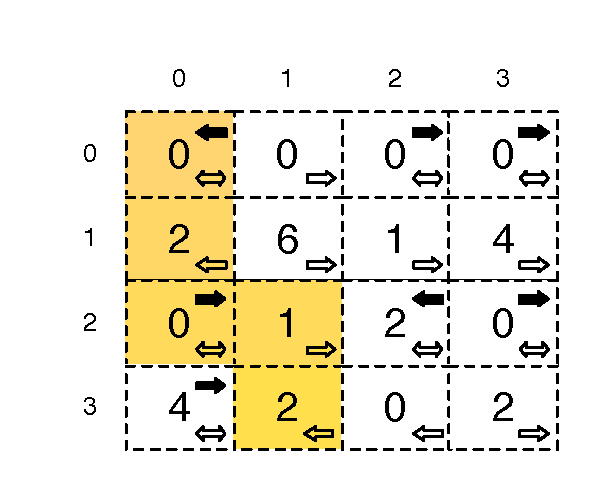
\includegraphics[scale=0.45]{Figs/robotMovesRewards.eps}\hspace{1em}\mbox{}}
%% \caption{A robot on a $4 \times 4$ grid} \label{fig:robot_game_grid}
%% \end{wrapfigure}
%% 
%% \noindent
En este modelo, \texttt{WIDTH} y \texttt{LENGTH} son constantes que definen la dimensión de la cuadrícula. \texttt{MOVES} es una matriz bidimensional que modela los posibles movimientos laterales en la cuadrícula (\texttt{0} permite que el robot se mueva solo hacia la izquierda, \texttt{1}, hacia cualquier lado y \texttt{2 }, solo a la derecha). Cuando la luz está en rojo (\texttt{light=0}) es el turno de la luz y puede escoger entre cambiar a amarillo (la transición etiquetada \texttt{l\_y}) o verde (la transición etiquetada \texttt{l\_g}). Observemis que cualquiera sea la elección, la luz puede fallar con probabilidad \texttt{Q}, en cuyo caso la luz se apaga (\texttt{light’=3}). Si la luz no está en rojo, entonces es el turno de Roborta. Si la luz está en amarillo (\texttt{light=1}) o está apagada (\texttt{light=3}), Roborta puede elegir moverse a la izquierda (\texttt{r\_l}) o a la derecha (\texttt{r\_r}), suponiendo que la matriz permite esos movimientos. Si la luz está en verde (\texttt{light=2}) o está apagada (\texttt{light=3}), Roborta puede elegir moverse hacia delante (en la figura sería hacia abajo), notemos que cuando \texttt{light=2} esta es a única alternativa. Al igual que la luz, cada elección de Roborta está sujeta a una probabilidad de falla (\texttt{P}), en cuyo caso, no puede realizar ningun movimiento y consume su turno (cambia el valor de \texttt{light} a 0). Vale la pena mencionar que omitimos en la Fig.~\ref{fig:robot_game_model} una matriz secundaria con las recompensas asignadas a cada posición.

%Las recompensas asignadas a cada ubicación de la cuadrícula se almacenan en una matriz llamada \texttt{REWARDS}.
La Figura~\ref{fig:robot_game_grid} muestra la asignación de recompensas a cada ubicación de la cuadrícula de $4 \times 4$, así como las restricciones de movimiento lateral (que se muestran en la parte inferior derecha de cada ubicación con flechas blancas).
El juego comienza en la ubicación $(0, 0)$ y se detiene cuando \roborta escapa por el final de la cuadrícula.


\begin{figure}
\centering
{\fontsize{6.6}{6.6}\selectfont\ttfamily
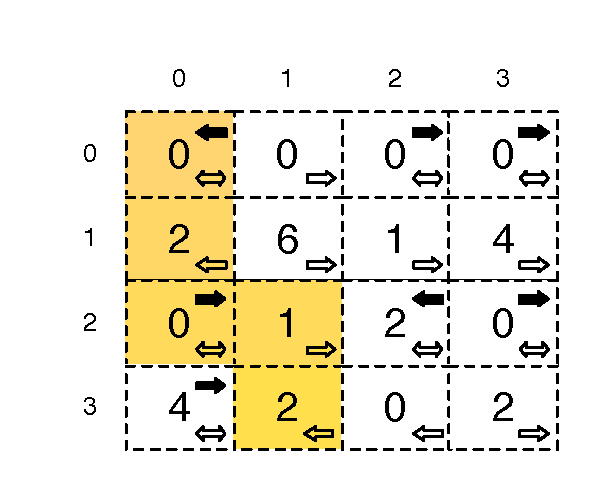
\includegraphics[scale=0.65]{Figs/robotMovesRewards.eps}\hspace{1em}\mbox{}}
\caption{\roborta en una matriz $4 \times 4$} \label{fig:robot_game_grid}
\end{figure}

Un escenario posible en este juego es el siguiente. \roborta comienza en la celda $(0,0)$ y, en un intento de minimizar las recompensas acumuladas por el robot, el entorno enciende la luz amarilla.
En aras de la simplicidad, asumimos que no hay fallas en la luz, es decir, $\texttt{Q}=0$.
Observemos que, si el ambiente juega siempre de esta manera (encendiendo la luz amarilla), entonces \roborta nunca alcanzará la meta y
el juego nunca terminaría. Este escenario ocurre cuando la luz juega de manera infair, es decir, una acción (la que enciende la luz verde) se habilita con infinita frecuencia, pero no se ejecuta con infinita frecuencia.
Suponiendo que el medio ambiente sea fair, podemos asegurar que finalmente se encenderá una luz verde, lo que permitirá que el robot avance.

Para el caso de \texttt{Q=0}, la mejor estrategia para \roborta cuando la luz es amarilla se muestra con flechas negras en la parte superior derecha de las celdas sin restricciones de movimiento.
% Como resultado, la mejor estrategia para lograr el objetivo del robot se puede observar en la parte resaltada de la cuadrícula en amarillo en
Como resultado, cuando ambos jugadores juegan sus estrategias óptimas, el camino tomado por \roborta para alcanzar la meta se puede observar en la Figura~\ref{fig:robot_game_grid} en la parte resaltada en amarillo de la cuadrícula. En la Sección \ref{sec:experimental_eval_fair}, evaluamos este problema experimentalmente con diferentes
configuraciones de este juego.
\section{Juegos Terminantes y Estrategias Fair}\label{sec:stopping_fair}

Comenzamos esta sección introduciendo las nociones de \emph{estrategia fair casi-seguras)} y \emph{juegos terminantes bajo fairness}. 
%%
%% It is worth noting that most of the definitions below  can be applied to both players. However, from now on, we assume that Player $2$ represents the environment,  which tries to minimize the amount of rewards obtained by the system, thus  fairness restrictions will be applied to this player. 
%%
De ahora en adelante, asumimos que el Jugador $2$ representa el ambiente, que trata de minimizar la cantidad de recompensas obtenidas por el sistema, por lo que se aplicarán restricciones de \textit{fairness} a este jugador.

%intuitively, one player represents the environment and the other represents the system. In our setting, the environment  wants to minimize the amount of rewards obtained by the system (clock ticks, bits successfully transmitted, etc), and the system wants to maximize these rewards. 
%In the following, we assume that Player $2$ is the environment, thus from now on fairness restrictions are applied to this player. 
\begin{definition}
Dado un juego estocástico $\StochG = (V, (V_1, V_2, V_\Probabilistic), \delta)$.
El conjunto de jugadas \textit{fair} del Jugador $2$ (denotado como $\FP^2$) se define de la siguiente manera:
\[
	\FP^2 = \{ \omega \in \GamePaths_{\StochG} \mid \forall v' \in V_2: v' \in \inf(\omega)  \Rightarrow \post(v') \subseteq \inf(\omega) \}
\]
%%    Given a stochastic game $\StochG = (V, (V_1, V_2, V_\Probabilistic), \delta)$ and  $i \in \{1,2\}$.
%% The set of fair plays for Player $i$ from vertex $v$ (denoted $\FP^i_v$) is defined as follows:
%% \[
%% 	\FP^i_v = \{ \omega \in \GamePaths_{\StochG,v} \mid \forall v' \in V_i: v' \in \inf(\omega)  \Rightarrow \post(v') \subseteq \inf(\omega) \}
%% \]
\end{definition}
Alternativamente, si consideramos a cada vértice como una proposición, el conjunto $\FP^2$ se puede escribir utilizando la notación {\LTL} como:
$\bigwedge_{v \in V_2} \bigwedge_{v' \in \post(v)}(\Box \Diamond v \Rightarrow \Box \Diamond v')$. Esta propiedad es $\omega$-regular, por lo que se puede medir en el $\sigma$-álgebra generada por los conos de $\GamePaths_{\StochG}$ (ver, por ejemplo, \cite[p.804]{BaierK08}) . Esta es una noción de \textit{fairness} basada en los estados, pero puede extenderse directamente a contextos donde se consideran las transiciones. En aras de la simplicidad, no lo hacemos en este trabajo.
	
%	Note that the set of fair plays is $\omega$-regular, thus it is measurable  in the $\sigma$-algebra generated by the cones of $\GamePaths_{\StochG}$ \cite{Katoen08}. 

%% The following definition introduces the notion of  (almost-sure) \emph{fair strategies} for Player $2$.
Luego, introducimos la noción de \emph{estrategias fair (casi-seguras)} para el Jugador $2$.
%% (Almost-sure) fair strategies for Player $1$ are defined analogously. 
\begin{definition} Dado un juego estocástico $\StochG = (V, (V_1, V_2, V_\Probabilistic), \delta)$,
una estrategia $\strat{2} \in \Strategies{2}$ se denomina \emph{casi-segura fair} (o simplemente \emph{fair}) si y solo si se cumple que:
%$\Prob{\strat{1}}{\strat{2}}_{\StochG,v}(\FP^2_v) = 1$,
$\Prob{\strat{1}}{\strat{2}}_{\StochG,v}(\FP^2) = 1$,
para toda $\strat{1} \in \Strategies{1}$ y $v \in V$. 
\end{definition}
%
El conjunto de todas las estrategias \textit{fair} para el Jugador $2$ se indica mediante $\FairStrats{2}$. Combinamos esta notación con la notación presentada en el Capítulo \ref{cap:preliminares}, por ejemplo, $\MemorylessFairStrats{2}$ se refiere al conjunto de todas las estrategias \textit{fair} y sin memoria para el Jugador $2$.
%
La definición anterior se basa en la noción de \textit{scheduler fair} tal como se introdujo para los procesos de decisión de Markov~\cite{DBLP:journals/dc/BaierK98,BaierK08}.

Tengamos en cuenta que para juegos terminantes, todas las estrategias son \textit{fair}, porque la probabilidad de visitar un vértice con infinita frecuencia es $0$.
%
También tengamos en cuenta que hay juegos que no son terminantes, pero se vuelven terminantes si el Jugador $2$ solo usa estrategias \textit{fair}. Esta es la idea principal detrás de la noción de \emph{terminante bajo fairness} tal como se presenta en la siguiente definición.

	
\begin{definition}\label{def:stopping-under-fairness}
  Un juego estocástico $\StochG = (V, (V_1, V_2, V_\Probabilistic), \delta)$ se dice que es \emph{terminante bajo fairness} si y solo si para todas las estrategias $\strat{1} \in \Strategies{1}, \strat{2} \in \FairStrats{2}$ y vértices $v \in V$, se cumple que
  $\Prob{\strat{1}}{\strat{2}}_{\StochG,v}(\Diamond T)=1$,  donde $T$ es el conjunto de vértices terminales de $\StochG$. 
\end{definition}

%\remarkPRD{Considerar agregar un ejemplo con \textbf{Roborta}}

%\subsection{Checking the stopping criteria}
\subsection{Verificación de criterios de parada.}

Esta sección está dedicada a la
caracterización efectiva de los juegos que se detienen bajo \textit{fairness}.
%% La siguiente parte de esta sección está dedicada a la efectiva
%% caracterización de los juegos que se detienen bajo la equidad.
El siguiente lema establece que, para cualquier juego que no sea terminante bajo
\textit{fairness}, existe una estrategia \emph{determinista sin memoria} para el Jugador 1 y una estrategia \textit{fair} para el Jugador 2 tal que se preserve su no-terminación.


\begin{lemma}\label{lm:memoryless-strat}
  Sea $\StochG = (V, (V_1, V_2, V_\Probabilistic), \delta)$ un juego estocástico, $v \in V$, y sea $T$ el conjunto de estados terminales en $\StochG$.
  %
  Si $\Prob{\strat{1}}{\strat{2}}_{\mathcal{G}, v}(\Diamond T) < 1$
  para alguna
  $\strat{1} \in \Strategies{1}$ y $\strat{2} \in \FairStrats{2}$,
  entonces, para alguna estrategia determinista y sin memoria
  $\strat{1}' \in \DetMemorylessStrats{1}$ y alguna estrategia \textit{fair}
  $\strat{2}' \in \FairStrats{2}$,
  $\Prob{\strat{1}'}{\strat{2}'}_{\mathcal{G}, v}(\Diamond T) < 1$.
\end{lemma}

La demostración de este lema se deduce notando que, si $\Prob{\strat{1}}{\strat{2}}_{\mathcal{G}, v}(\Diamond T) < 1$, tiene que haber un camino finito que conduce con cierta probabilidad a un componente final que no contiene un estado terminal y que es una trampa para la estrategia \textit{fair} $\strat{2}$. Esta parte del juego permite la construcción de una estrategia determinista sin memoria para el Jugador 1 al asegurarse de que sigue el mismo camino finito (pero omitiendo bucles) y que atrapa al Jugador 2 en el mismo componente final.
% PRUEBA PASADA AL APENDICE
\iffalse
\begin{proof}
  Fijemos las estrategias $\strat{1} \in \Strategies{1}$, $\strat{2} \in
  \FairStrats{2}$ y un vértice $v \in V$ tales que
  $\Prob{\strat{1}}{\strat{2}}_{\mathcal{G}, v}(\Diamond T) < 1$.
  Observemos que que podemos definir un MDP (que llamamos $\StochG^{V_1{+}V_2}$) a partir de
  $\StochG$ considerando que $V_1$ y $V_2$ pertenecen al mismo jugador.  Para este MDP consideremos el conjunto $U = \{ (V',\delta')
  \mid(V',\delta') \in \EndComp(\StochG^{V_1{+}V_2}) \text{ y }
  V'\cap T = \emptyset \}$ de los componentes finales que no contienen vértices terminales. Entonces, definimos una estrategia para este jugador al combinar
  $\strat{1}$ y $\strat{2}$ (la cual llamaremos $\strat{1}{+}\strat{2}$) de la siguiente manera
  : se comporta como $\strat{1}$ en los caminos finitos cuyos últimos estados pertenecen a $V_1$, y se comporta como $\strat{2}$ en los caminos finitos cuyos últimos estados pertenecen a $V_2$. Observemos que tenemos que
  $\MDPProb{\strat{1}{+}\strat{2}}_{\StochG^{V_1+V_2},v}(\Diamond T) <
  1$. Por las propiedades de límite de los MDPs (Teorema 10.120 \cite{BaierK08})
  tenemos que:
  %
  \begin{equation}\label{lm:memoryless-strat-eq1}
    \MDPProb{\strat{1}{+}\strat{2}}_{\StochG^{V_1+V_2},v} \left(\{ \omega \in \MDPPaths{\strat{1}{+}\strat{2}}_{\StochG^{V_1+V_2},v} \mid \limit(\omega)  \in U \}\right) > 0,
  \end{equation}
  %
  donde $\limit(\omega)$ denota la componente final que se repite con infinita frecuencia en $\omega$, como se define en \cite{BaierK08}.  Notemos que
  , el hecho de que $\strat{2}$ sea \textit{fair} y
  (\ref{lm:memoryless-strat-eq1}) implican que hay una componente final alcanzable $\EC{C}= (V',\delta') \in U$ tal que, para todo
  $v' \in V_2 \cap V'$, $\post^\delta(v') \subseteq V'$ $(\dag)$.
  %
  Esto se puede demostrar por contradicción: si $(\dag)$ no vale tenemos que para todo componente final en $U$ tiene que existir
  algún vértice en
  $V_2$ tal que algunos de sus sucesores no estén en el componente; pero,
  como $\strat{2}$ es \textit{fair}, tendríamos que
  %
  $\MDPProb{\strat{1}{+}\strat{2}}_{\StochG^{V_1+V_2},v} \left ( \{ \omega \in \MDPPaths{\strat{1}{+}\strat{2}}_{\StochG^{V_1+V_2},v} \mid \limit(\omega) \in U \}\right) = 0$
  %
  contradiciendo (\ref{lm:memoryless-strat-eq1}). Por lo tanto $(\dag)$ debe valer.

  Por consiguiente, existe algún camino finito $\hat{\omega} = v_0 v_1 v_2 \dots v_k$
  en este MDP tal que $v_i \notin T$ para todo $i$, $v_k \in V'$, y
  $\MDPProb{\strat{1}{+}\strat{2}}_{\StochG^{V_1+V_2},v}(v_0\dots v_k) > 0$.

  Ahora bien, definimos $\strat{1}'$ de la siguiente manera:
  %
  $\strat{1}'(v') = \hat{\omega}_{i+1}$, si $i < k$ es el índice mas grande tal que $v' = \hat{\omega}_{i}$;
  %
  $\strat{1}'(v') = v''$ para algún $v'' \in
  V'\cap\post^\delta(v)$ arbitrario, si $v' \in V'$;
  %
  en otro caso $\strat{1}'(v') = v''$ para algún
  $v'' \in \post^\delta(v')$ arbitrario.
  %
  $\strat{2}'$ se define usando una distribución uniforme, es decir:
  $\strat{2}'(v')(v'') = \frac{1}{\# \post^\delta(v')}$, para todo $v'
  \in V_2$ y $v'' \in \post^\delta(v')$.
  
  $\strat{1}'$ se define de tal modo que salta adelante de $\hat{\omega}$
  evitando todos los bucles que $\strat{1}$ pueda introducir.  Sea
  $\hat{\omega}{\downharpoonleft}_{\strat{1}'}$ el camino finito obtenido al seguir $\hat{\omega}$ salteando todos los bucles de acuerdo a $\strat{1}'$.
  %
  Observemos que $\hat{\omega}{\downharpoonleft}_{\strat{1}'}$ es un camino válido en $\StochG$, que todavía termina en el estado $v_k$, y que
  $\MDPProb{\strat{1}',\strat{2}'}_{\StochG,v}({\hat{\omega}{\downharpoonleft}_{\strat{1}'}})>0$.
  Además, por ($\dag$) y por la definición de $\strat{1}'$, tenemos que $\MDPProb{\strat{1}',\strat{2}'}_{\StochG, v_k}(\Box V') = 1$.
  Por lo tanto $\MDPProb{\strat{1}',\strat{2}'}_{\StochG, v}(\Diamond T) < 1$.
  Además, notemos que $\strat{1}'$ es estacionaria y $\strat{2}'$
  es fair.
%%   Now, we define $\strat{1}'$ as follows: $\strat{1}'(v') = \hat{\omega}_{i+1}$, if $v' = \hat{\omega}_{i}$ for some $i <k$; 
%% $\strat{1}'(v') = v''$ for some arbitrary $v'' \in \post^\delta(v')$, if $v' \neq \hat{\omega}_{i}$ for all $i \leq k$ and $v' \notin V'$; $\strat{1}'(v') = v''$ for some arbitrary $v'' \in V'\cap \post^\delta(v)$, if
%% $v' \in V'$. $\strat{2}'$ is defined as the uniform strategy, that is: $\strat{2}'(v')(v'') = \frac{1}{\# \post^\delta(v')}$, for every $v' \in V_2$ and $v'' \in \post^\delta(v')$. Note that, $\MDPProb{\strat{1}',\strat{2}'}_{\StochG,v}(v_0\dots v_k) >0$, and 
%% also (by definition of $\strat{1}'$ and ($\dag$)) we have that $\MDPProb{\strat{1}',\strat{2}'}_{\StochG, v_k}(\Box V') = 1$, thus $\MDPProb{\strat{1}',\strat{2}'}_{\StochG, v}(\Diamond T) < 1$. Furthermore, note that $\strat{1}'$ is memoryless and $\strat{2}'$ is fair.%we can define strategies
%% %$\strat{1}'$ and $\strat{2}'$ such that they collaborate to reach $\EC{C}$, and for any vertex $\hat{v} \in V_1 \cap V'$ we set 
%% %$\strat{1}'(\hat{v})=v'$ (for some $v' \in V'$); while $\strat{2}'$ behaves as $\strat{2}$ in nodes belonging to $V_2$. Note that this
%% %ensures that $\strat{2}'$ is fair and $\strat{1}'$ is memoryless. Since the probability of reaching $\EC{C}$ is positive, and no node in $T$ is reached when playing $\strat{1}'$ and $%\strat{2}'$,  we get that $\Prob{\strat{1}'}{\strat{2}'}_{\StochG, v}(\Diamond T) < 1$.
\qedhere
\end{proof}
\fi


El siguiente teorema establece que la verificación de la terminación bajo \textit{fairness} en un juego estocástico $\StochG$ se puede reducir a verificar los criterios de parada en un MDP, que se obtiene de $\StochG$ al fijar una estrategia en el Jugador 2 que seleccione entre las transiciones de salida de acuerdo a una
distribución uniforme. Por lo tanto, este teorema permite una solución basada en grafos para determinar la detención bajo \textit{fairness}.

%The next theorem is central to reduce the problem of checking whether a game is stopping to that of checking whether an MDP version of it is stopping.

\begin{theorem}\label{thm:uniform-prob}
  Sea $\StochG = (V, (V_1, V_2, V_\Probabilistic), \delta)$ un juego estocástico y sea $T$ su conjunto de estados terminales.
  Consideremos la estrategia (sin memoria) del Jugador $2$
  $\uniformstrat{2} : V_2 \rightarrow \Dist(V)$ definida como
  $\uniformstrat{2}(v)(v') = \frac{1}{\# \post(v)}$, para todo $v \in
  V_2$ y $v' \in post(v)$.
  %
  Entonces, $\StochG$ es terminante bajo \textit{fairness} si y solo si
  $\Prob{\strat{1}}{\uniformstrat{2}}_{\StochG,v}(\Diamond T)=1$ para
  todo $v\in V$ y $\strat{1} \in \Strategies{1}$.
%% Then, for all $v \in V$ it holds that:  $\Prob{\strat{1}}{\strat{2}}_{\StochG,v}(\Diamond T)=1$, for 
%% every  $\strat{1} \in \Strategies{1}$ and fair $\strat{2} \in \FairStrats{2}$, iff  
%% $\Prob{\strat{1}}{\uniformstrat{2}}_{\StochG,v}(\Diamond T)=1$ for every $\strat{1} \in \Strategies{1}$.
\end{theorem}

Mientras que la parte ``solo si'' del teorema es directa, la parte ``si'' se prueba por
contraposición usando el lema~\ref{lm:memoryless-strat}.

% PRUEBA PASADA AL APENDICE
\iffalse
\begin{proof}
``Si'': Supongamos que $\Prob{\strat{1}}{\uniformstrat{2}}_{\StochG,v}(\Diamond T)=1$ para toda estrategia $\strat{1}$ del Jugador $1$.  Además, 
asumamos por contradicción, que
$\Prob{\strat{1}'}{\strat{2}'}_{\StochG,v}(\Diamond T) < 1$ para alguna $\strat{1}'\in \Strategies{1}$ y alguna $\strat{2}'\in \FairStrats{2}$. 
Por el Lema \ref{lm:memoryless-strat}, podemos asumir de forma segura que $\strat{1}'$ es estacionaria y determinista.
Por lo tanto, al fijar $\strat{1}'$, obtenemos un proceso de decisión de Markov (finito) denotado por $\StochG^{\strat{1}'}$.
Por asunción, tenemos que
$\inf_{\strat{2} \in \FairStrats{2}} \MDPProb{\strat{2}}_{\StochG^{\strat{1}'},v}(\Diamond T) < 1 $. Adicionalmente, por el Teorema 10.133 en \cite{BaierK08}, tenemos que $\inf_{ \strat{2} \in \FairStrats{2}}\MDPProb{\strat{2}}_{\StochG^{\strat{1}'},v}(\Diamond T) = 1 - \sup_{\strat{2} \in \FairStrats{2}} \MDPProb{\strat{2}}_{\StochG^{\strat{1}'},v}(\neg T \U U)$, donde $T$ es el conjunto de estados terminales,  $\neg T$ es su complemento, y
$U = \bigcup \{ V' \mid (V', \delta') \in \EndComp(\StochG^{\strat{1}'}) \text{ y }  T \cap V' = \emptyset\}$.
%Furthermore, in \cite{BaierK08} it is shown how we can define a fair strategy that maximizes the probabilities. 
Sea $\strat{2}''$ la estrategia \textit{fair} que maximiza el valor de $\MDPProb{\strat{2}''}_{\StochG^{\strat{1}'},v}(\neg T \U U)$, el cual existe como se ha demostrado en la prueba del Teorema 10.133 en \cite{BaierK08}.
Entonces tenemos que $\MDPProb{\strat{2}''}_{\StochG^{\strat{1}'},v}(\neg T \U U) > 0$ y por lo tanto existe
un camino $v_0 v_1 \dots v_n$ con probabilidad positiva tal que $v_i \notin T$ y $v_n$ pertenece a un componente final $\EC{C} = (V'', \delta'')$
tal que $T \cap V'' = \emptyset$. Como $\strat{2}''$ es \textit{fair}, por nuestra definición de estrategia \textit{fair}, el componente final $\EC{C}$ contiene todas las transiciones en $\StochG^{\strat{1}'}$ cuando se lo restringe a $V''$.
% when restricted  to $\EC{C}$. 
Por lo tanto, $\MDPProb{\uniformstrat{2}}_{\StochG^{\strat{1}'},v}(\Diamond V'') > 0$, y 
$\MDPProb{\uniformstrat{2}}_{\StochG^{\strat{1}'},v''}(\Box V'') = 1 $ 
desde cualquier estado en $v'' \in V''$, lo cual implica que $\MDPProb{\uniformstrat{2}}_{\StochG{\strat{1}'},v}(\neg T \U V'') > 0$. 
Entonces, $\MDPProb{\uniformstrat{2}}_{\StochG^{\strat{1}'},v}(\Diamond T) < 1$, lo cual contradice nuestro supuesto inicial.

\noindent ``Solo si'': Esta parte de la demostración es directa ya que $\uniformstrat{2}$ es una estrategia \textit{fair}.
%Suppose that  $\Prob{\strat{1}}{\strat{2}}(\mathcal{A})=1$ for 
%every $\strat{1} \in \Strategies{1}$ and  $\strat{2} \in \FairStrats{2}$, and 
%$\Prob{\strat{1}'}{\starredstrat{2}}(\mathcal{A})<1$, for some Verifier's strategy $\strat{1}'$, that is, there is a path 
%$v_0, v_1, \dots, v_n$ in the Markov chain $\StochG^{\strat{1}', \starredstrat{2}}$ such that $v_i \notin T$ and 
%$v_n \in B$ for some BSCC $B$ satisfying $T \cap B = \emptyset$. By the definition of $\starredstrat{2}$, $B$ is also a 
%maximal end component in the MDP  $\StochG^{\strat{1}'}$. 
%Thus, we can define a fair strategy $\strat{2}'$ that takes path 
%$v_0, \dots, v_n$ in   $\StochG^{\strat{1}'}$ and afterwards behaves in a fair way in the maximal end-component $B$, since 
%$T \cap B = \emptyset$ we have $\Prob{\strat{1}'}{\strat{2}'}(\mathcal{A})<1$ which contradicts our initial assumption.
\qedhere
\end{proof} 
\fi

El teorema~\ref{thm:uniform-prob} introduce un algoritmo para verificar que el juego estocástico $\StochG$ es terminante bajo \textit{fairness}: transformar
$\StochG$ en un MDP $\StochG^{\uniformstrat{2}}$ al fijar
$\uniformstrat{2}$ en $\StochG$ y verificar si
$\MDPProb{\strat{1}}_{\StochG^{\uniformstrat{2}},v}(\Diamond T)=1$ para todo $v\in V$.
%
Consecuentemente, tenemos el siguiente teorema.

\begin{theorem}\label{thm:fair-is-poly}
  Verificar si un juego estocástico $\StochG$ es terminante bajo
  \textit{fairness} o no tiene complejidad $O(\poly(\size(\StochG)))$.
\end{theorem}

%% In practice, one needs some procedure to check whether a stochastic
%% game is stopping under fairness. As already remarked above, a game
%% could be not stopping for all pairs of strategies, but it could be
%% stopping when fairness assumptions are made about Player $2$'s
%% behavior.
%% %
%% One could use Theorem~\ref{thm:uniform-prob} to transform game
%% $\StochG$ into the MDP $\StochG^{\uniformstrat{2}}$ by fixing
%% $\uniformstrat{2}$ in $\StochG$ and check whether
%% $\MDPProb{\strat{1}}_{\StochG^{\uniformstrat{2}},v}(\Diamond T)=1$ for
%% all $v\in V$.  Instead, we use Theorem~\ref{thm:uniform-prob} to

%\remarkPRD{este ultimo pedacito de la subsecci\'on es el primer candidato a volar si es necesario}
Alternativamente, podemos usar el teorema~\ref{thm:uniform-prob} para proporcionar un
algoritmo que trabaje directamente sobre $\StochG$ lo cual evita la construcción del
MDP intermedio.
%
La idea principal es utilizar una modificación del operador $\pre$
estándar, como se muestra en la siguiente definición:

%
\begin{align*}
  %% \EFairpre(C) \ = \ {}&\{ v \in V \mid \delta(v,C) > 0\} \\
  %% \AFairpre(C) \ = \ {}&\{ v \in V_2\cup V_\Probabilistic \mid \delta(v,C)>0\} \\
  %%                      &\cup \ \{ v \in  V_1 \mid \forall v' \in V : \delta(v,v') > 0 \Rightarrow v' \in C \}
  \EFairpre(C) = {}&\{ v \in V \mid \delta(v,C) > 0\} \\
  \AFairpre(C) = {}&\{ v \in V_2{\cup} V_\Probabilistic \mid \delta(v,C)>0\} \\ 
                       &\cup \{ v \in  V_1 \mid \forall v' {\in} V : \delta(v,v') > 0 \Rightarrow v' {\in} C \}
\end{align*}
%% \remarkPC{Esta parte confunde a los reviewers, no entiende para que es necesaria dada que ya trnasformandolo a un MDP podemos usar teoria de MDPs}
Como de costumbre, consideramos las clausuras transitivas de estos operadores, denotados $\EFairpre^*$ y $\AFairpre^*$, respectivamente.
%% These operators allows us to check if a given game is stopping under fairness for the strategy $\uniformstrat{2}$, as defined in Theorem \ref{thm:uniform-prob}.
%
\begin{theorem}\label{thm:stopping-algorithm}
  Sea $\StochG = (V, (V_1, V_2, V_\Probabilistic), \delta)$, un juego estocástico y sea $T$ el conjunto de sus estados terminales. Entonces,
  %% $\Prob{\strat{1}}{\strat{2}}_{\StochG,v}(\Diamond T) = 1$ for every
  %% $\strat{1} \in \Strategies{1}$ and $\strat{2} \in \FairStrats{2}$
  %% iff $v \in V\setminus \EFairpre^*(V \setminus \AFairpre^*(T))$.
  \begin{enumerate}[(1)]
  \item%
    $\Prob{\strat{1}}{\strat{2}}_{\StochG,v}(\Diamond T) = 1$ para todo
    $\strat{1} \in \Strategies{1}$ y $\strat{2} \in \FairStrats{2}$
    si y solo si $v \in V\setminus \EFairpre^*(V \setminus \AFairpre^*(T))$, y
  \item%
    $\StochG$ es terminante bajo \textit{fairness} si y solo si
    $\EFairpre^*(V \setminus \AFairpre^*(T)) = \emptyset$.
  \end{enumerate}
\end{theorem}

\begin{proof}
  (2) es una consecuencia inmediata de (1). Por lo que solo probamos la primer declaración.

  Observemos que 
  $\StochG^{\uniformstrat{2}} = (V, (V_1, \emptyset, {V_2 \cup V_\Probabilistic}), \delta')$,
  donde $\delta'(v,\cdot)=\delta(v,\cdot)$ si $v\in V_1\cup V_\Probabilistic$
  y $\delta'(v,\cdot)=\uniformstrat{2}(v)$ si $v\in V_2$.
  %
  En este MDP, los operadores $\Apre$ y $\Epre$ se definen como
  \begin{align*}
    \Epre(C) \ = \ {}&\{ v \in V \mid \delta'(v,C) > 0\} \\
    \Apre(C) \ = \ {}&\{ v \in V_2\cup V_\Probabilistic \mid \delta'(v,C) > 0\} \\
		     &\cup \ \{ v \in  V_1 \mid \forall v' \in V : \delta'(v,v') > 0 \Rightarrow v' \in C \}
  \end{align*}
  %
  Es directo verificar que $\EFairpre(C)=\Epre(C)$ y
  $\AFairpre(C)=\Apre(C)$ para cualquier $C\subseteq V$.

  Como consecuencia de esta observación y por el Teorema~\ref{thm:uniform-prob}, basta con comprobar que
  $\MDPProb{\strat{1}}_{\StochG^{\uniformstrat{2}},v}(\Diamond T)=1$ para toda estrategia $\strat{1}$ si y solo si
  $v \in V\setminus \Epre^*(V \setminus \Apre^*(T))$ $(\ddag)$.

  Por el Lema~10.110~\cite{BaierK08}, $v\in V \setminus \Apre^*(T)$ si y solo si
  $\exists \strat{1}\colon \MDPProb{\strat{1}}_{\StochG^{\uniformstrat{2}},v}(\Diamond T) = 0$.
  Por lo tanto, $v\in V \setminus \Apre^*(T)$ si y solo si
  $\exists \strat{1}\colon \MDPProb{\strat{1}}_{\StochG^{\uniformstrat{2}},v}(\Box \neg T) = 1$.
  Teniendo en cuenta que todos los estados terminales son absorbentes, tenemos por el Lema~10.111~\cite{BaierK08}, $v\in \Epre^*(V \setminus \Apre^*(T))$ si y solo si
  $\exists \strat{1}\colon \MDPProb{\strat{1}}_{\StochG^{\uniformstrat{2}},v}(\Diamond T) < 1$
  de lo cual se deduce $(\ddag)$.
  \qedhere
\end{proof}



%% It is direct to see that $\EFairpre$ and $\AFairpre$ can be computed using standard graph algorithms which are polynomial in time w.r.t.\ the size of the game, thus we obtain the following theorem.

%% \begin{theorem}\label{thm:fair-is-poly}
%%   Checking whether the stochastic game $\StochG$ is stopping under
%%   fairness or not is in $O(\poly(\size(\StochG)))$.
%% \end{theorem}

%% \begin{theorem}\label{thm:fair-is-poly}
%%   Given a stochastic game $\StochG = (V, (V_1, V_2, V_\Probabilistic), \delta)$, it can be checked in time $O(\poly(\size(\StochG)))$ whether $\StochG$ is almost-sure stopping under fairness or not.
%% \end{theorem}

%	One main property in game theory is determinacy. Intuitively, if a game is determined each vertex has a value for the players. Another intuitive reading of determinacy is that the prior knowledge of the opponent's strategy gives us no advantage. 
	
%\subsection{Determinacy of Stopping Games under Fairness}
\subsection{Determinación de Juegos Terminantes bajo Fairness.}
%	As briefly mentioned in the introduction, the determinacy of a large class of games was established by  Martin in \cite{Martin98}, in particular, the determinacy of stochastic games with payoff functions that are Borel and bounded follows from Martin's results. The objective  function $\Rewards$ is unbounded, so Martin's theorems cannot be applied to these kinds of functions. In \cite{FilarV96}, the determinacy of stopping stochastic games with total rewards objective functions is proven for stopping games, but note that here we restrict the class of strategies that Player $2$ can use, and thus the value of the game  may change. In the following we prove that this restriction does not affect the determinacy of the  games.

%As briefly mentioned in the introduction, t

La determinación de los juegos estocásticos con funciones de \textit{payoff} Borel-medibles acotadas se deriva de los resultados de Martin~\cite{Martin98}. Debido a que nos enfocamos en la función de \textit{payoff} de \emph{recompensa total acumulada}, es decir: $\Rewards(\omega) = \sum^\infty_{i=0}\reward(\omega_i)$, y la misma no está acotada, los teoremas de Martin no se aplican a ella. En \cite{FilarV96}, se prueba la determinación de una clase general de juegos estocásticos terminantes (llamados \emph{transitorios}) con recompensas totales. Sin embargo, tengamos en cuenta que restringimos al Jugador $2$ para que solo juegue con estrategias \textit{fair} y, por lo tanto, el último resultado tampoco se aplica.
%
En \cite{PatekBertsekas99} los autores clasifican las estrategias del Jugador $2$ en \emph{adecuadas} (aquellas que aseguran la terminación) e \emph{inadecuadas} (aquellas que prolongan el juego indefinidamente). Para probar la determinación, los autores asumen que el valor del juego para las estrategias inadecuadas del Jugador $2$ es $\infty$. Vale la pena señalar que, para probar los resultados a continuación, no hacemos ninguna asunción sobre estrategias \textit{unfair}.
%\remarkPC{Quizas estos comentarios puedan ir en related work, sino podríamos agregar algo the shortest stochastic games.}\remarkPRD{A mi me parece que est\'a bien que se diga aqu\'i aunque se repita en el related work}
%
A continuación demostramos que restringir a jugadas \textit{fair} no afecta la determinación de los juegos.
%ADD ROADMAP TO PROOFS
\begin{figure}
  \centering
  %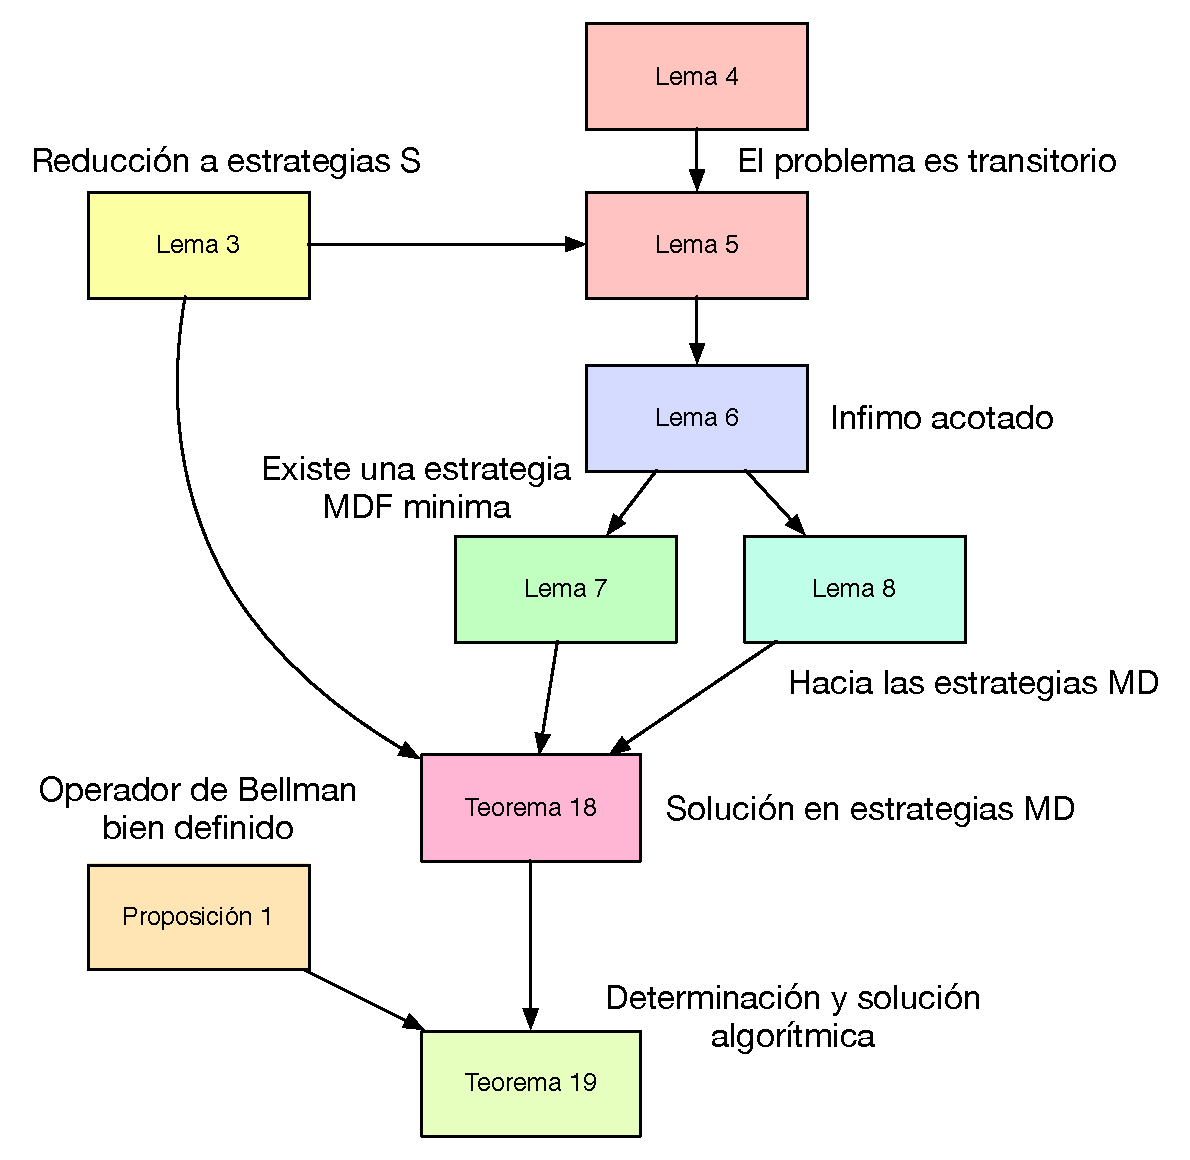
\includegraphics[scale=0.5]{Figs/roadmap.pdf}
  \scalebox{1.2}{%
    \begin{tikzpicture}[on grid,auto,align at top]
      \node[] (l2ul) [] {};
      \node[] (l2lr) [below right=0.5 and 1.4 of l2ul] {};
      \node[] (l3ul) [right=3.6 of l2ul] {};
      \node[] (l3lr) [below right=1.2 and 1.4 of l3ul] {};
      \node[] (l5ul) [below=1.4 of l3ul] {};
      \node[] (l5lr) [below right=0.5 and 1.4 of l5ul] {};
      \node[] (l6ul) [below left=0.7 and 0.9 of l5ul] {};
      \node[] (l6lr) [below right=0.5 and 1.4 of l6ul] {};
      \node[] (l7ul) [below right=0.7 and 0.9 of l5ul] {};
      \node[] (l7lr) [below right=0.5 and 1.4 of l7ul] {};
      \node[] (p1ul) [below=2.9 of l2ul] {};
      \node[] (p1lr) [below right=0.5 and 1.4 of p1ul] {};
      \node[] (t4ul) [below left=0.8 and 0.9 of l6ul] {};
      \node[] (t4lr) [below right=0.5 and 1.4 of t4ul] {};
      \node[] (t5ul) [below=0.7 of t4ul] {};
      \node[] (t5lr) [below right=0.5 and 1.4 of t5ul] {};


      \draw[color=yellow!40,fill=yellow!40] (l2ul) rectangle (l2lr);
      \draw[color=red!20,fill=red!20] (l3ul) rectangle (l3lr);
      \draw[color=orange!20,fill=orange!20] (l5ul) rectangle (l5lr);
      \draw[color=violet!20,fill=violet!20] (l6ul) rectangle (l6lr);
      \draw[color=magenta!20,fill=magenta!20] (l7ul) rectangle (l7lr);
      \draw[color=lime!40,fill=lime!40] (p1ul) rectangle (p1lr);
      \draw[color=blue!20,fill=blue!20] (t4ul) rectangle (t4lr);
      \draw[color=green!20,fill=green!20] (t5ul) rectangle (t5lr);
      
      \node[] (l2) [below right=0.25 and 0.7 of l2ul] {Lem.~\ref{lm:semimarkov2}};
      \node[] (l3) [right=3.6 of l2] {Lem.~\ref{lm:bound-prob-stationary-strats}};
      \node[] (l4) [below=0.7 of l3] {Lem.~\ref{lm:games-are-bounded}};
      \node[] (l5) [below=0.7 of l4] {Lem.~\ref{lm:memoryless-strat-p2-bounded-expectation}};
      \node[] (l6) [below left=0.7 and 0.9 of l5] {Lem.~\ref{lm:infima-in-dmf}};
      \node[] (l7) [below right=0.7 and 0.9 of l5] {Lem.~\ref{lm:semimarkov-to-detmemoryless}};
      \node[] (p1) [below=2.9 of l2] {Prop.~\ref{pn:continuity}};
      \node[] (t4) [below left=0.8 and 0.9 of l6] {Teo.~\ref{thm:reduce-to-memoryless}};
      \node[] (t5) [below=0.7 of t4] {Teo.~\ref{thm:game-determinacy}};

      \path[->]
      (l2) edge[] ([xshift=-4ex,yshift=0.5ex]l4)
      (l3) edge[] (l4)
      (l4) edge[] (l5)
      (l5) edge[] (l6)
      (l5) edge[] (l7)
      (l2) edge[] ([xshift=-2.5ex,yshift=1.3ex]t4)
      (l6) edge[] (t4)
      (l7) edge[] (t4)
      (p1) edge[] (t5)
      (t4) edge[] (t5)
      ;

      \node[] () [above right=0.5 and 1.8 of l2] {\parbox{6.9em}{\flushleft Reducción a estrategias $\mathit{S}$}};
      \node[] () [below right=0.15 and 1.8 of l3] {\parbox{6.5em}{\flushleft El problema es transitorio}};
      \node[] () [above right=0.1 and 1.8 of l5] {\parbox{6.5em}{\flushleft El ínfimo está acotado}};
      \node[] () [above left=0.95 and 0.75 of l6] {\parbox{5.2em}{\flushleft Existe estrategia min. $\mathit{MD}\mathcal{F}$}};
      \node[] () [below right=0.4 and 1.4 of l7] {\parbox{6.8em}{\flushleft En camino a estrategias $\mathit{MD}$}};
      \node[] () [above right=0.9 and 0.1 of p1] {\parbox{7.5em}{\flushleft Op. de Bellman bien definido}};
      \node[] () [above right=0.05 and 2 of t4] {\parbox{7.5em}{\flushleft Solución en estrategias $\mathit{MD}$}};
      \node[] () [below right=0.15 and 2.4 of t5] {\parbox{10.6em}{\flushleft Determinación y solución algorítmica}};
      
    \end{tikzpicture}
  }
  \caption{Una guía para la prueba de los teoremas~\ref{thm:reduce-to-memoryless} y~\ref{thm:game-determinacy}}\label{fig:roadmap}
\end{figure}


La Figura~\ref{fig:roadmap} muestra las dependencias de los lemas que eventualmente llevan a nuestros resultados principales, específicamente, el Teorema~\ref{thm:reduce-to-memoryless}, el cual establece que el problema general queda delimitado a estrategias deterministas sin memoria, y el Teorema~\ref{thm:game-determinacy}, el cual establece la determinación y la corrección de la solución algorítmica a través de las ecuaciones de Bellman.
Para demostrar el Teorema~\ref{thm:reduce-to-memoryless} utilizamos la noción intermedia de estrategias \emph{semi-Markovianas} \cite{FilarV96} y un primer paso para esta reducción se presenta en el Lema~~\ref{lm:semimarkov2}.
Los Lemas~\ref{lm:bound-prob-stationary-strats}
y~\ref{lm:games-are-bounded} aseguran las características transitorias de los problemas que se detienen bajo \textit{fairness}.  Estos lemas son esenciales para probar que cada recompensa total posible tiene solución
(Lema~\ref{lm:memoryless-strat-p2-bounded-expectation}).  Ya acercándonos al Teorema~\ref{thm:reduce-to-memoryless},
El Lema~\ref{lm:infima-in-dmf} establece que siempre existe una estrategia minimizadora \textit{fair} que es estacionaria y determinista, y
el Lema~\ref{lm:semimarkov-to-detmemoryless} ayuda a reducir el problema del dominio de las estrategias semi-Markovianas al dominio de las estrategias sin memoria deterministas.  Utilizando el Teorema~\ref{thm:reduce-to-memoryless}
y la Proposición~\ref{pn:continuity}, la cual establece que las ecuaciones de Bellman se comportan bien en el retículo de soluciones,
El Teorema~\ref{thm:game-determinacy} finalmente queda demostrado.
La noción de estrategias \emph{semi-Markov} \cite{FilarV96} será importante para los teoremas de esta sección. Intuitivamente, una estrategia semi-Markov solo tiene en cuenta la longitud de una jugada, el estado inicial y el estado actual para seleccionar el siguiente paso en la jugada.
%In some sense, it possesses a very limited memory, a counter.
        
\begin{definition}\label{def:semimarkov:strategy} Sea $\StochG = (V, (V_1, V_2, V_\Probabilistic), \delta)$ un juego estocástico. Una estrategia $\strat{i} \in \Strategies{i}$ se denomina semi-Markov si: $\strat{i}(v \hat{\omega}v') = \strat{i}(v \hat{\omega}'v')$, para todo $v \in V$ y $\hat{\omega}, \hat{\omega}' \in V^*$ tal que $|\hat{\omega}|=|\hat{\omega}'|$. 
\end{definition}

Observemos que, al fijar un estado inicial $v$, una estrategia semi-Markov $\strat{i}$ puede considerarse como una secuencia de estrategias sin memoria $\strat{i}^{0,v}\strat{i }^{1,v}\strat{i}^{2,v}\ldots$ donde $\strat{i}(v)=\strat{i}^{0,v}(v)$ y $\strat{i}(v\hat{\omega}v')=\strat{i}^{|\hat{\omega}|+1,v}(v')$. El conjunto de todas las estrategias semi-Markov (resp. semi-Markov \textit{fair}) para el Jugador $i$ se denomina $\SemiMarkovStrats{i}$ (resp. $\SemiMarkovFairStrats{i}$).

La importancia de las estrategias semi-Markov radica en el hecho de que, cuando el Jugador $2$ juega una estrategia semi-Markov, cualquier estrategia del Jugador $1$ puede ser imitada por una estrategia semi-Markov como se establece en el siguiente teorema.

\begin{lemma}\label{lm:semimarkov2}
  Sea $\StochG$ un juego estocástico bajo \textit{fairness},  y sea
  $\strat{2} \in \SemiMarkovFairStrats{2}$ una estrategia semi-Markov
  \textit{fair}. Entonces, para toda $\strat{1} \in \Strategies{1}$, existe una estrategia
  semi-Markov $\starredstrat{1} \in \SemiMarkovStrats{1}$
  tal que
  $\Expect{\strat{1}}{\strat{2}}_{\StochG, v}[\Rewards] =
  \Expect{\starredstrat{1}}{\strat{2}}_{\StochG, v}[\Rewards]$.
\end{lemma}
%
\iffalse
\begin{proof}[Sketch]
  The proof follows the arguments of Theorem 4.2.7 in \cite{FilarV96}
  adapted to our setting.
  %We sketch the proof, the details can be found in the Appendix.
	
  Consider the event $\Diamond^{k} v' = \{ \omega \in
  \GamePaths_\StochG \mid \omega_k = v'\}$, for $k\geq 0$. That is,
  the set of runs in which $v'$ is reached after exactly $k$ steps.
  %
  We define $\starredstrat{1}$ as follows.
  \[
  \starredstrat{1}(\hat{\omega}v')(v'') =  \Prob{\strat{1}}{\strat{2}}_{\StochG,v}(\Diamond^{k+1} v'' \mid \Diamond^k v') 
  \]
  %
  for every $\hat{\omega}$ such that $\Prob{\strat{1}}{\strat{2}}_{\StochG,v}(\hat{\omega}v') > 0$ and $|\hat{\omega}v'| = k$.  For those $\hat{\omega}$'s with $\Prob{\strat{1}}{\strat{2}}_{\StochG,v}(\hat{\omega}v') = 0$ we define $\starredstrat{1}(\hat{\omega}v')$ to be any arbitrary distribution.
  %
  Notice that $\starredstrat{1}$ is a semi-Markov strategy.
  %
  We prove that $\starredstrat{1}$ is the strategy that satisfies the
  conclusion of the theorem.
  %
  For this, we first show that $\Prob{\strat{1}}{\strat{2}}_{\StochG,v}(\Diamond^{k} v') = \Prob{\starredstrat{1}}{\strat{2}}_{\StochG,v}(\Diamond^{k} v')$ by induction on $k$, and use it to conclude the following. 
% \textcolor{red}{   \remarkPC{La parte roja  esta mal y no es necesaria}
%  Using this result, we prove that $\Prob{\strat{1}}{\strat{2}}_{\StochG,v}(\Diamond^{k+1} v' \mid \Diamond^k v'') = \Prob{\starredstrat{1}}{\strat{2}}_{\StochG,v}(\Diamond^{k+1} v' \mid \Diamond^k v'')$.
  %
%  Now, for every $v_0 \dots v_k$ with $v_0=v$,
  %
 % $\Prob{\strat{1}}{\strat{2}}_{\StochG,v}(v_0 \dots v_k)
 % = {\prod^{k-1}_{i=0} \Prob{\strat{1}}{\strat{2}}_{\StochG,v}(\Diamond^{i+1} v_{i+1} \mid \Diamond^i v_i)}
 % = \prod^{k-1}_{i=0} \Prob{\starredstrat{1}}{\strat{2}}_{\StochG,v}(\Diamond^{i+1} v_{i+1} \mid \Diamond^i v_i)
 % = \Prob{\starredstrat{1}}{\strat{2}}_{\StochG,v}(v_0 \dots v_k)$,  
 % and, for the case in which $v_0\neq v$,
 % $\Prob{\strat{1}}{\strat{2}}_{\StochG,v}(v_0 \dots v_k) = 0
 % = \Prob{\starredstrat{1}}{\strat{2}}_{\StochG,v}(v_0 \dots v_k)$.
  %
 % Therefore, for every $\hat{\omega}\in V^*$,
  %$\Prob{\strat{1}}{\strat{2}}_{\StochG,v}(\hat{\omega}) 
 % = \Prob{\starredstrat{1}}{\strat{2}}_{\StochG,v}(\hat{\omega})$ and
  %from this last equality,
 % $\Expect{\strat{1}}{\strat{2}}_{\StochG,v}[\Rewards] = \Expect{\starredstrat{1}}{\strat{2}}_{\StochG,v}[\Rewards]$ follows.
  %}
  \begin{align*}
  \Expect{\strat{1}}{\strat{2}}_{\StochG,v}[\Rewards]   &  = \sum^\infty_{N=0} \sum_{\hat{\omega} \in V^{N+1}} \Prob{\strat{1}}{\strat{2}}_{\StochG,v}(\hat{\omega})\reward(\hat{\omega}_N)
   = \sum^\infty_{N=0} \sum_{v' \in V} \Prob{\strat{1}}{\strat{2}}_{\StochG,v}(\Diamond^N v')\reward(v') \\
  & =  \sum^\infty_{N=0} \sum_{v' \in V} \Prob{\starredstrat{1}}{\strat{2}}_{\StochG,v}(\Diamond^N v')\reward(v') 
   = \Expect{\starredstrat{1}}{\strat{2}}_{\StochG,v}[\Rewards] \tag*{\qedhere}
  \end{align*}

%\qed
\end{proof}
\fi
% PRUEBA PASADA AL APENDICE
\iffalse
\begin{proof}
  Consideremos el evento $\Diamond^{k} v' = \{ \omega \in
  \GamePaths_\StochG \mid \omega_k = v'\}$, para $k\geq 0$. Es decir,
  el conjunto de corridas en las cuales $v'$ es alcanzado en exactamente $k$ pasos.
  %
  Definimos $\starredstrat{1}$ de la siguiente manera:
  \[
  \starredstrat{1}(\hat{\omega}v')(v'') =  \Prob{\strat{1}}{\strat{2}}_{\StochG,v}(\Diamond^{k+1} v'' \mid \Diamond^k v') 
  \]
  para todo $\hat{\omega}$ tal que
  $\Prob{\strat{1}}{\strat{2}}_{\StochG,v}(\hat{\omega}v') > 0$ y
  $|\hat{\omega}v'| = k$.  Para $\hat{\omega}$ con
  $\Prob{\strat{1}}{\strat{2}}_{\StochG,v}(\hat{\omega}v') = 0$ definimos $\starredstrat{1}(\hat{\omega}v')$ como una distribución arbitraria cualquiera.
  %for $|\hat{\omega}v'| = k$.

  Probamos que esta estrategia satisface las condiciones del teorema.
  Primero, demostramos que
  %
  \begin{equation}\label{equ:diamondk}
    \Prob{\strat{1}}{\strat{2}}_{\StochG,v}(\Diamond^{k} v') =
    \Prob{\starredstrat{1}}{\strat{2}}_{\StochG,v}(\Diamond^{k} v').
  \end{equation}
  %
  Notemos que para $k=0$ tenemos que,
  \[\Prob{\strat{1}}{\strat{2}}_{\StochG,v}(\Diamond^{0} v') =
  \Prob{\strat{1}}{\strat{2}}_{\StochG,v}(v') = \Delta_v(v') =
  \Prob{\starredstrat{1}}{\strat{2}}_{\StochG,v}(v')=
  \Prob{\starredstrat{1}}{\strat{2}}_{\StochG,v}(\Diamond^{0} v').\]
  %
  Para $k + 1 > 0$, notamos que
  \[
  \Prob{\strat{1}}{\strat{2}}_{\StochG,v}(\Diamond^{k+1} v') = \sum_{\hat{\omega} \in V^{k+1}} \Prob{\strat{1}}{\strat{2}}_{\StochG,v}(\hat{\omega}v')  = \sum_{v'' \in \pre(v')}\sum_{\hat{\omega} \in V^k} \Prob{\strat{1}}{\strat{2}}_{\StochG,v}(\hat{\omega}v''v'),
  \] 
  y por lo tanto, para este caso, basta con mostrar que, para todo
  $v''\in\pre(v)$,
  %
  \[
    \sum_{\hat{\omega} \in V^k} \Prob{\strat{1}}{\strat{2}}_{\StochG,v}(\hat{\omega}v''v') = \sum_{\hat{\omega} \in V^k} \Prob{\starredstrat{1}}{\strat{2}}_{\StochG,v}(\hat{\omega}v''v').
  \]

  La prueba usa inducción en $k$ haciendo análisis por casos. Observamos que
  el caso base sigue de manera similar al caso inductivo y lo señalaremos debidamente cuando corresponda.
  %
  Si $v'' \in V_2$, procedemos de la siguiente manera.
  %
  \begin{align}	
    \label{lm:semimarkov2-eq1-l1}
    \sum_{\hat{\omega} \in V^k}\Prob{\strat{1}}{\strat{2}}_{\StochG,v}(\hat{\omega}v''v')
    & = \sum_{\hat{\omega} \in V^k}\Prob{\strat{1}}{\strat{2}}_{\StochG,v}(\hat{\omega}v'') \strat{2}(\hat{\omega}v'')(v')\\
    \label{lm:semimarkov2-eq1-l2}
    & = \alpha \sum_{\hat{\omega} \in V^k}\Prob{\strat{1}}{\strat{2}}_{\StochG,v}(\hat{\omega}v'') \\
    \label{lm:semimarkov2-eq1-l3}
    & = \alpha \sum_{\hat{\omega} \in V^k}\Prob{\starredstrat{1}}{\strat{2}}_{\StochG,v}(\hat{\omega}v'') \\
    \label{lm:semimarkov2-eq1-l4}
    & = \sum_{\hat{\omega} \in V^k}\Prob{\starredstrat{1}}{\strat{2}}_{\StochG,v}(\hat{\omega}v''v')
  \end{align}
  %
  (\ref{lm:semimarkov2-eq1-l1}) se deduce por definición.
  %
  Para (\ref{lm:semimarkov2-eq1-l2}), definimos $\alpha =
  \strat{2}(\hat{\omega}v'')(v')$ si $\hat{\omega}$ comienza en $v$. Al recordar que la naturaleza semi-Markoviana de $\strat{2}$ define el
  mismo $\alpha$ para cualquier $\hat{\omega}\in V^k$ a partir de $v$, y que
  $\Prob{\strat{1}}{\strat{2}}_{\StochG,v}(\hat{\omega}v'') = 0$ si
  $\hat{\omega}$ no comienza en $v$, $\alpha$ resulta ser factor común.
  %
  (\ref{lm:semimarkov2-eq1-l3}) se deriva ya sea por hipótesis inductiva, o, en el caso base, al observar que
  $\Prob{\strat{1}}{\strat{2}}_{\StochG,v}(v'') =
  \Delta_v(v'')=\Prob{\starredstrat{1}}{\strat{2}}_{\StochG,v}(v'')$.
  %
  (\ref{lm:semimarkov2-eq1-l4}) resuelve tal y como
  (\ref{lm:semimarkov2-eq1-l2}).

  Para el caso en el que $v'' \in V_1$, procedemos de la siguiente manera.
  %
  \begin{align}	
    \sum_{\hat{\omega} \in V^k}\Prob{\strat{1}}{\strat{2}}_{\StochG,v}(\hat{\omega}v''v') \hspace{-6em} & \notag\\
    \label{lm:semimarkov2-eq2-l1}
    & = \sum_{\hat{\omega} \in V^k}\Prob{\strat{1}}{\strat{2}}_{\StochG,v}(\hat{\omega}v'') \strat{1}(\hat{\omega}v'')(v')\\
    \label{lm:semimarkov2-eq2-l2}
    & = \left( \sum_{\hat{\omega} \in V^k}\Prob{\strat{1}}{\strat{2}}_{\StochG,v}(\hat{\omega}v'') \right) \frac{\displaystyle\sum_{\hat{\omega} \in V^k}\Prob{\strat{1}}{\strat{2}}_{\StochG,v}(\hat{\omega}v'') \strat{1}(\hat{\omega}v'')(v')}{\displaystyle\sum_{\hat{\omega} \in V^k}\Prob{\strat{1}}{\strat{2}}_{\StochG,v}(\hat{\omega}v'')} \\
    \label{lm:semimarkov2-eq2-l3}
    & = \sum_{\hat{\omega} \in V^k}\Prob{\strat{1}}{\strat{2}}_{\StochG,v}(\hat{\omega}v'') \Prob{\strat{1}}{\strat{2}}_{\StochG,v}(\Diamond^{k+1} v' \mid \Diamond^k v'') \\
    \label{lm:semimarkov2-eq2-l4}
    & = \sum_{\hat{\omega} \in V^k}\Prob{\starredstrat{1}}{\strat{2}}_{\StochG,v}(\hat{\omega}v'') \starredstrat{1}(\hat{\omega}v'')(v)\\
    \label{lm:semimarkov2-eq2-l5}
    & = \sum_{\hat{\omega} \in V^k}\Prob{\starredstrat{1}}{\strat{2}}_{\StochG,v}(\hat{\omega}v''v')
  \end{align}
  %
  (\ref{lm:semimarkov2-eq2-l1}) se deduce por definición.
  %
  (\ref{lm:semimarkov2-eq2-l2}) se obtiene al multiplicar y dividir el término por
  $\sum_{\hat{\omega}v'' \in V^k}\Prob{\strat{1}}{\strat{2}}_{\StochG,v}(\hat{\omega}v'')$.
  %
  (\ref{lm:semimarkov2-eq2-l3}) se deduce de la definición de probabilidad condicional al observar que
  $\Prob{\strat{1}}{\strat{2}}_{\StochG,v}({\Diamond^{k+1} v'} \cap {\Diamond^k v''}) =
  \sum_{\hat{\omega} \in V^k}\Prob{\strat{1}}{\strat{2}}_{\StochG,v}(\hat{\omega}v'') \strat{1}(\hat{\omega}v'')(v')$
  y 
  $\Prob{\strat{1}}{\strat{2}}_{\StochG,v}(\Diamond^{k} v'') =
  \sum_{\hat{\omega} \in V^k}\Prob{\strat{1}}{\strat{2}}_{\StochG,v}(\hat{\omega}v'')$.
  %
  Finalmente, (\ref{lm:semimarkov2-eq2-l4}) se deduce por la definición de
  $\starredstrat{1}$ y (\ref{lm:semimarkov2-eq2-l5}) por la definición de 
  $\Prob{\starredstrat{1}}{\strat{2}}_{\StochG,v}$.

  La prueba para el caso $v'' \in V_\Probabilistic$ se deduce de igual manera que para el primer caso, con la diferencia de que en vez de considerar
  $\strat{2}(\hat{\omega}v'')(v')$ necesitamos considerar
  $\delta(v'',v')$.



  Usando (\ref{equ:diamondk}), podemos realizar el cálculo de la siguiente manera
  %
  \begin{align}
  \Expect{\strat{1}}{\strat{2}}_{\StochG,v}[\Rewards]   &  = \sum^\infty_{N=0} \sum_{\hat{\omega} \in V^{N+1}} \Prob{\strat{1}}{\strat{2}}_{\StochG,v}(\hat{\omega})\reward(\hat{\omega}_N) \label{equ:expect:semimarkov:a}\\
  & = \sum^\infty_{N=0} \sum_{v' \in V} \Prob{\strat{1}}{\strat{2}}_{\StochG,v}(\Diamond^N v')\reward(v') \label{equ:expect:semimarkov:b}\\
  & =  \sum^\infty_{N=0} \sum_{v' \in V} \Prob{\starredstrat{1}}{\strat{2}}_{\StochG,v}(\Diamond^N v')\reward(v') \label{equ:expect:semimarkov:c}\\
  &  = \Expect{\starredstrat{1}}{\strat{2}}_{\StochG,v}[\Rewards] \label{equ:expect:semimarkov:d}
  \end{align}
  %
  La igualdad (\ref{equ:expect:semimarkov:a}) se deriva del hecho que 
  $\Expect{\strat{1}}{\strat{2}}_{\StochG,v}[\Rewards]= \reward(v) + \xi(v)(v') \cdot \Expect{\strat{1}}{\strat{2}}_{\StochG,v'}[\Rewards]$
  con $\xi(v)(v')=\strat{1}(v)(v')$ si $v\in V_1$,
  $\xi(v)(v')=\strat{2}(v)(v')$ si $v\in V_2$, y $\xi(v)(v')=\delta(v,v')$
  si $v\in V_\Probabilistic$.
  %
  La igualdad (\ref{equ:expect:semimarkov:b}) se deduce por
  $\Prob{\strat{1}}{\strat{2}}_{\StochG,v}(\Diamond^N v')=\sum_{\hat{\omega} \in V^{N}v'} \Prob{\strat{1}}{\strat{2}}_{\StochG,v}(\hat{\omega})$.
  %
  (\ref{equ:expect:semimarkov:c}) es el resultado de aplicar
  (\ref{equ:diamondk}).
  %
  Siguiendo la misma lógica que antes nos da (\ref{equ:expect:semimarkov:d}).
\qedhere
\end{proof}
\fi
%
%%First, we prove  that, if Player 1 plays in a memoryless way,  Player 2 can restrict herself to memoryless fair strategies, without affecting the result of the game.


En un juego terminante, todos los estados no terminales son transitorios (un estado es
transitorio si el tiempo esperado que ambos jugadores pasan en él es
finito). De hecho, \cite{FilarV96}~define un juego terminante con
estados terminales en $T$ como un \emph{juego transitorio}, es decir, un juego en
que $\sum^\infty_{N=1} \sum_{\hat{\omega} \in (V \setminus T)^{N}}
\Prob{\strat{1}}{\strat{2}}_{\StochG,v}(\hat{\omega}) < \infty$ para
todas las estrategias $\strat{1}\in\Strategies{1}$ y $\strat{2}\in\Strategies{2}$.
%
Obviamente, esta generalidad no se cumple en nuestro caso ya que las
estrategias unfair hacen que el juego se mantenga infinitamente en un conjunto de estados no terminales.
%
Por lo tanto, probamos una propiedad más débil en nuestro contexto. En lineas generales,
el siguiente lema establece que, en los juegos que terminan bajo \textit{fairness},
%% el tiempo esperado que ambos jugadores pasan en estados no terminales es
%% finito, dado que los dos jugadores juegan estrategias sin memoria, y en
%% en particular, que Player~2 juega fair.
los estados no terminales son transitorios, siempre que los dos jugadores jueguen
estrategias sin memoria, y en particular, que Jugador $2$ solo juegue de forma
\textit{fair}.

\begin{lemma}\label{lm:bound-prob-stationary-strats}
  Sea $\StochG = (V, (V_1, V_2, V_\Probabilistic), \delta)$ un juego estocástico que es terminante bajo \textit{fairness} siendo $T$ su conjunto de estados terminales.
  %
  Sea $\strat{1} \in \MemorylessStrats{1}$ una estrategia sin memoria para
  el Jugador $1$ y $\strat{2} \in \MemorylessFairStrats{2}$ una
  estrategia \textit{fair} sin memoria para el Jugador $2$.  Entonces
  %\[
  $\sum^\infty_{N=1} \sum_{\hat{\omega} \in (V \setminus T)^{N}} \Prob{\strat{1}}{\strat{2}}_{\StochG,v}(\hat{\omega}) < \infty$.
  %\]
\end{lemma}

\begin{proof}
  Como $\strat{1}$ y $\strat{2}$ son estacionarias, podemos fijar estas estrategias
  y obtener una cadena de Markov finita absorbente
  $\StochG^{\strat{1},\strat{2}} = (V, (\emptyset,\emptyset, V_1 \cup V_2 \cup V_P), \delta^{\strat{1}, \strat{2}})$,
  entonces el resultado se deduce de las propiedades básicas de las cadenas de Markov. En aras de la completitud, damos a continuación una prueba.
  
  Sea $|V|$ la cantidad de estados de la cadena de Markov
  $\StochG^{\strat{1},\strat{2}}$ y sea $T$ su conjunto de vértices terminales.
  %
  Como $\Prob{\strat{1}}{\strat{2}}_{\StochG,v}(\Diamond T) = 1$
  y la cadena de Markov es finita, desde cualquier vértice tenemos un camino de longitud $k$
  con $k \leq|V|$ hacia un vértice terminal.
  %
  Además, sea
  $\lambda = \min \{ \delta^{\strat{1},\strat{2}}(v,v') > 0 \mid v,v' \in V \}$,
  el cual está bien definido ya que $\StochG^{\strat{1},\strat{2}}$ tiene una cantidad finita de estados.
  Por lo tanto, para cualquier $N\geq 0$ tenemos:
  %
  \[
  \sum_{\hat{\omega} \in (V \setminus T)^{N+1}} \Prob{\strat{1}}{\strat{2}}_{\StochG,v}(\hat{\omega}) \leq (1 - \lambda^{|V|})^{\left\lfloor{\frac{N}{|V|}}\right\rfloor}
  \]
  %% \[
  %% \sum_{\hat{\omega} \in v(V \setminus T)^N} \Prob{\strat{1}}{\strat{2}}_{\StochG,v}(\hat{\omega}) < (1 - \lambda^{|V|})^N
  %% \]
  Por lo tanto, si $\lambda<1$,
  \begin{align*}
    \sum^\infty_{N=0}\sum_{\hat{\omega} \in (V \setminus T)^{N+1}} \Prob{\strat{1}}{\strat{2}}_{\StochG,v}(\hat{\omega}) & \ \leq \ \sum^{\infty}_{N=0}(1 - \lambda^{|V|})^{\left\lfloor{\frac{N}{|V|}}\right\rfloor} \\
    & \ = \ {|V|}\sum^{\infty}_{i=0}(1 - \lambda^{|V|})^i \ = \ \frac{|V|}{1 - \lambda^{|V|}}.
  \end{align*}
  Si $\lambda = 1$, es fácil comprobar que
  $\sum^\infty_{N=0}\sum_{\hat{\omega} \in (V \setminus T)^{N+1}} \Prob{\strat{1}}{\strat{2}}_{\StochG,v}(\hat{\omega}) \leq {|V|}$.
  \qedhere
\end{proof}

Este resultado se puede extender a todas las estrategias del Jugador $1$. La idea principal detrás de la prueba es fijar una estrategia \textit{fair} estacionaria para
el Jugador $2$ (por ejemplo, una estrategia que use la distribución uniforme). Esto produce un MDP
que se detiene para cada estrategia del Jugador $1$, y además, puede ser
visto como un \emph{juego transitorio} de un solo jugador (como se define en
\cite{FilarV96}). Por lo tanto, el resultado se deduce del Lema
\ref{lm:bound-prob-stationary-strats} y el Teorema 4.2.12 en
\cite{FilarV96}.

\begin{lemma}\label{lm:games-are-bounded}
  Sea $\StochG$ un juego estocástico que es terminante bajo \textit{fairness}
  y sea $T$ el conjunto de estados terminales. Adicionalmente, sea
  $\strat{1} \in \Strategies{1}$ una estrategia para el Jugador $1$ y
  $\strat{2} \in \MemorylessFairStrats{2}$ una estrategia \textit{fair} y sin memoria para el Jugador $2$.  Entonces
  %\[
  $\sum^\infty_{N=0} \sum_{\hat{\omega} \in v(V \setminus T)^N} \Prob{\strat{1}}{\strat{2}}_{\StochG,v}(\hat{\omega}) < \infty$.
  %\]
\end{lemma}
% PRUEBA PASADA AL APENDICE
\iffalse
\begin{proof}
  En lugar de realizar las reducciones apropiadas para aplicar el Teorema 4.2.12 de \cite[p.~174]{FilarV96}, realizamos una prueba directa basada en las ideas
  de la prueba de ese teorema.
  
  Fijemos una estrategia \textit{fair} $\strat{2} \in \MemorylessFairStrats{2}$ y
  consideremos el MDP
  $\StochG^{\strat{2}} = (V, (V_1, \emptyset, V_2 \cup V_\Probabilistic), \delta^{\strat{2}})$.
  %
  Definimos el siguiente funcional:
  %\remarkPRD{No deberia ser $v \in (V_2 \cup V_\Probabilistic)\setminus T$?}
  %
  \[
  \Gamma'(f)(v) =
  \begin{cases}
    1 + \sum_{v' \in \post(v)} \delta^{\strat{2}}(v,v')  f(v') & \text{ si } v \in (V_2 \cup V_\Probabilistic) \setminus T  \\
    \max \{1  + f(v') \mid v' \in \post(v) \} & \text{ si } v \in  V_1 \setminus T \\
    0 & \text{ si } v \in T.
  \end{cases}
  \]
  %
  %\textcolor{red}{It is well-known that, since $\StochG^{\strat{2}}$ is stopping, this
  %functional is a contraction mapping and then it has a unique
  %fixpoint (see, e.g., proof of Theorem 4.2.6 in \cite{FilarV96}),
  %which gives us the optimal value for Player~1 in MDP
  %$\StochG^{\strat{2}}$.  Let $\mu \Gamma'$ denote the fixpoint of $\Gamma'$.}
  
  Observemos que por el Lema \ref{lm:bound-prob-stationary-strats} y por el Teorema 4.2.2 de \cite{FilarV96},  $\StochG^{\strat{2}}$
  es un juego transitorio de 1 jugador. Por lo tanto, por el Teorema 4.2.6 de \cite{FilarV96} $\Gamma'$ es un \textit{mapping de contracción} y tiene un punto fijo único (denotado $\mu \Gamma' \in [0,\mathbb{R}]^V$), el cual a su vez es la solución del juego.
  
  Como $\mu \Gamma'(v_n)$ es el valor óptimo para un vértice dado $v_{n}$ tenemos que:
 % \remarkPRD{para que esto sea cierto me parece que se necesita que la primera l\'inea en la definici\'on de $\Gamma'$ sea $1+\sum_{v' \in \post(v)} \delta^{\strat{2}}(v,v')  f(v')$}
  %
  \begin{equation}\label{eq:lm:games-are-bounded-eq1}
    \mu \Gamma'(v_n) \geq 1 + \sum_{v_{n+1} \in \post(v_n)} \delta^{\strat{1}^n, \strat{2}}(v_n, v_{n+1}) \mu \Gamma'(v_{n+1})
  \end{equation}
  %
  para cualquier estrategia sin memoria $\strat{1}^n$ (el valor obtenido a partir del punto fijo es
  óptimo entre las estrategias sin memoria, por lo que no puede mejorar con  $\strat{1}^n$).
  %
  Tomemos cualquier secuencia $\hat{\omega} = v_0 \dots v_n$ con
  $\hat{\omega}_n = v_n$ y multipliquemos
  (\ref{eq:lm:games-are-bounded-eq1}) por
  $\prod^{n-1}_{i=0} \delta^{\strat{1}^i, \strat{2}}(\hat{\omega}_i, \hat{\omega}_{i+1})$
  en ambos lados. Esto nos da
  %
  \begin{align}
    \prod^{n-1}_{i=0} \delta^{\strat{1}^i, \strat{2}}(\hat{\omega}_i, \hat{\omega}_{i+1}) \mu \Gamma'(\hat{\omega}_n)  \hspace{-6.5em}& \notag\\
    \geq \ & \prod^{n-1}_{i=0} \delta^{\strat{1}^i, \strat{2}}(\hat{\omega}_i, \hat{\omega}_{i+1}) \label{eq:lm:games-are-bounded-eq2} \\
    & + \ \prod^{n-1}_{i=0} \delta^{\strat{1}^i, \strat{2}}(\hat{\omega}_i, \hat{\omega}_{i+1})\sum_{v_{n+1} \in \post(v_n)} \delta^{\strat{1}^n, \strat{2}}(v_n, v_{n+1}) \mu \Gamma'(v_{n+1}) \notag
  \end{align}
  %
  En la ecuación de arriba, asumimos que
  $\prod^{-1}_{i=0} \delta^{\strat{1}^i, \strat{2}}(\hat{\omega}_i, \hat{\omega}_{i+1}) = 1$
  para el caso en que $n=0$.
  
  Considerando todas las secuencias de longitud $n+1$ en $v(V \setminus T)^n$,
  a partir de (\ref{eq:lm:games-are-bounded-eq2}), y reescribiendo la última linea de la desigualdad, obtenemos
  %
  \begin{align}
    \sum_{\hat{\omega} \in v(V \setminus T)^n}\prod^{n-1}_{i=0} \delta^{\strat{1}^i, \strat{2}}(\hat{\omega}_i, \hat{\omega}_{i+1}) \mu \Gamma'(\hat{\omega}_n)  \hspace{-5.5em}& \notag\\
    \geq \ & \sum_{\hat{\omega} \in v(V \setminus T)^n}\prod^{n-1}_{i=0} \delta^{\strat{1}^i, \strat{2}}(\hat{\omega}_i, \hat{\omega}_{i+1}) \label{eq:lm:games-are-bounded-eq3}\\
    & + \ \sum_{\hat{\omega} \in v(V \setminus T)^{n+1}}(\prod^{n}_{i=0} \delta^{\strat{1}^i, \strat{2}}(\hat{\omega}_i, \hat{\omega}_{i+1}) \mu \Gamma'(\hat{\omega}_{n+1})) \notag
  \end{align}
  %
  Sumando todas las posibles secuencias hasta $N$ obtenemos
  \begin{align}
    \sum^{N}_{n=0}\sum_{\hat{\omega} \in v(V \setminus T)^n}\prod^{n-1}_{i=0} \delta^{\strat{1}^i, \strat{2}}(\hat{\omega}_i, \hat{\omega}_{i+1}) \mu \Gamma'(\hat{\omega}_n)   \hspace{-6.5em}& \notag\\
    \geq \ & \sum^{N}_{n=0} \sum_{\hat{\omega} \in v(V \setminus T)^n}\prod^{n-1}_{i=0} \delta^{\strat{1}^i, \strat{2}}(\hat{\omega}_i, \hat{\omega}_{i+1}) \label{eq:lm:games-are-bounded-eq4} \\
    & + \ \sum^{N}_{n=0} \sum_{\hat{\omega} \in v(V \setminus T)^{n+1}}(\prod^{n}_{i=0} \delta^{\strat{1}^i, \strat{2}}(\hat{\omega}_i, \hat{\omega}_{i+1}) \mu \Gamma'(\hat{\omega}_{n+1})) \notag
  \end{align}
  %
  (\ref{eq:lm:games-are-bounded-eq4}) puede ser reescrito equivalentemente como
  \begin{align}
    \sum^{N}_{n=0}\sum_{\hat{\omega} \in v(V \setminus T)^n}\prod^{n-1}_{i=0} \delta^{\strat{1}^i, \strat{2}}(\hat{\omega}_i, \hat{\omega}_{i+1}) \mu \Gamma'(\hat{\omega}_n)  \hspace{-6.5em}& \notag\\
    \geq \ & \sum^{N}_{n=0} \sum_{\hat{\omega} \in v(V \setminus T)^n}\prod^{n-1}_{i=0} \delta^{\strat{1}^i, \strat{2}}(\hat{\omega}_i, \hat{\omega}_{i+1}) \label{eq:lm:games-are-bounded-eq5}\\
    & + \ \sum^{N+1}_{n=1} \sum_{\hat{\omega} \in v(V \setminus T)^{n}}(\prod^{n-1}_{i=0} \delta^{\strat{1}^i, \strat{2}}(\hat{\omega}_i, \hat{\omega}_{i+1}) \mu \Gamma'(\hat{\omega}_{n})) \notag
  \end{align}
  %
  Al sustraer
  $\sum^{N+1}_{n=1} \sum_{\hat{\omega} \in v(V \setminus T)^{n}}(\prod^{n-1}_{i=0} \delta^{\strat{1}^i, \strat{2}}(\hat{\omega}_i, \hat{\omega}_{i+1}) \mu \Gamma' (v_{n}))$
  de ambos lados de la desigualdad
  (\ref{eq:lm:games-are-bounded-eq5}), obtenemos
  %
  \begin{align}
    \label{eq:lm:games-are-bounded-eq6}
    \mu \Gamma'(v)  - \sum_{\hat{\omega} \in v(V \setminus T)^{N+1}}\prod^{N}_{i=0} \delta^{\strat{1}^i, \strat{2}}(\hat{\omega}_i,\hat{\omega}_{i+1}) \mu \Gamma'(\hat{\omega}_{N+1})  \hspace{-6.5em}& \\
    \geq \ & \sum^{N}_{n=0} \sum_{\hat{\omega} \in v(V \setminus T)^n}\prod^{n-1}_{i=0} \delta^{\strat{1}^i, \strat{2}}(\hat{\omega}_i, \hat{\omega}_{i+1}) \notag
  \end{align}
  %
  Aplicando límites a ambos lados de la desigualdad
  (\ref{eq:lm:games-are-bounded-eq6}) obtenemos
  %
  \begin{align}
    \label{eq:lm:games-are-bounded-eq7}
    \mu \Gamma(v)  - \lim_{N \to \infty} \sum_{\hat{\omega} \in v(V \setminus T)^{N+1}}\prod^{N}_{i=0} \delta^{\strat{1}^i, \strat{2}}(\hat{\omega}_i,\hat{\omega}_{i+1}) \mu \Gamma'(\hat{\omega}_{N+1})  \hspace{-8.5em}& \\
    \geq \ & \lim_{N \to \infty} \sum^{N}_{n=0} \sum_{\hat{\omega} \in v(V \setminus T)^n}\prod^{n-1}_{i=0} \delta^{\strat{1}^i, \strat{2}}(\hat{\omega}_i, \hat{\omega}_{i+1}) \notag
  \end{align}
  %
  %\remarkPRD{No entiendo como aplica el Lemma~\ref{lm:bound-prob-stationary-strats}  aqu\'i. Me parece que $\Gamma'$ deber\'ia ser distinto para poder aplicar el lemma.}
  Ahora,  $\mu \Gamma'(v) \in \mathbb{R}^V$ es acotado para todo $v$. Adicionalmente,
  \[
  \lim_{N \to \infty}\sum_{\hat{\omega} \in v(V \setminus T)^{N+1}}\prod^{N}_{i=0} \delta^{\strat{1}^i, \strat{2}}(\hat{\omega}_i,\hat{\omega}_{i+1}) \nu(\hat{\omega}_{N+1}) = 0,
  \]
  %
  Por lo tanto, el término derecho de la desigualdad
  (\ref{eq:lm:games-are-bounded-eq7}) es un número finito.  Esto significa que
  para toda secuencia de estrategias sin memoria
  $\strat{1}^0,\strat{1}^1, \dots$ obtenemos
  %
  \[
  \lim_{N \to \infty} \sum^{N}_{n=0} \sum_{\hat{\omega} \in v(V \setminus T)^n}\prod^{n-1}_{i=0} \delta^{\strat{1}^i, \strat{2}}(\hat{\omega}_i, \hat{\omega}_{i+1}) < \infty,
  \]
  %
  Observando que cualquier estrategia semi-Markoviana $\strat{1}'$ puede pensarse como una
  secuencia de estrategias sin memoria, se deduce que
  \[
  \lim_{N \to \infty} \sum^{N}_{n=0} \sum_{\hat{\omega} \in v(V \setminus T)^n} \MDPProb{\strat{1}'}_{\StochG^{\strat{2}}, v}(\hat{\omega}) < \infty,
  \]
  %
  para toda $\strat{1}'$ semi-Markoviana.  Además, como toda
  estrategia $\strat{1}$ tiene una estrategia semi-Markoviana equivalente (ver prueba del Lema \ref{lm:semimarkov2}), el resultado se deduce.
  %\remarkPRD{Quiz'as esta parte e la prueba del Theorem \ref{lm:semimarkov2} necesite un lema aparte(Esto es a modo de comentario, no para hacer ahora)}
% First, we describe how a  stochastic game as defined in this paper can be equivalently defined as a \emph{transient game} as defined in \cite{FilarV96}.
%A transient game consists of a finite set of states $S$, for each state $s \in S$, $A^i(s)$ is a finite set of actions for Player $i$ (for $i \in \{0,1\}$).  A probabilistic transition function noted $p(s' \mid s, a_1,a_2)$ giving the probability of reaching state $s'$ from state $s$ when actions $a_1 \in A_1$ and $a_2 \in A_2$ are selected, and a reward function $r(s,a_1,a_2) \in \mathbb{R}$ given the rewards obtained if actions $a_1$ and $a_2$ are executed from state $s$.  A strategy for Player $1$ is a 
%sequence $f_0,f_1,\dots$ of functions $f : S^* A^1 A^2 S \rightarrow  \Dist$
  \qedhere
\end{proof}
\fi


%% %\remarkPRD{@Pablo: Revis\'a bien lo que escrib\'i en este p\'arrafo!!}
%% Using the previous theorem, some fairly simple calculations lead to
%% the fact that the value of the total accumulated reward payoff game is
%% well-defined for any strategy of the players.  This is stated in the
%% next theorem.

%% \begin{theorem}\label{thm:memoryless-strat-p2-bounded-expectation}
%%   Let $\StochG= (V, (V_1, V_2, V_\Probabilistic), \delta)$ be a
%%   stochastic game that is stopping under fairness,
%%   $\strat{1} \in \Strategies{1}$ a strategy for Player~1, and
%%   $\strat{2} \in \FairStrats{2}$ a fair strategy for Player~2.
%%   Then, for all $v \in V$,
%%   $\Expect{\strat{1}}{\strat{2}}_{\StochG,v}[\Rewards] < \infty$.
%% \end{theorem}

%% As a consequence of this theorem, the value of the game is bounded
%% from above for any Player $1$'s strategy.
%% \remarkPC{Sacar el corolario 1 y usar el Teorema 6, los reviewers de TACAS se quejaron de que es directo y gasta espacio}
%% \begin{corollary}\label{coro:inf-for-strat2-is-bounded}
%%   Let $\StochG= (V, (V_1, V_2, V_\Probabilistic), \delta)$ be a
%%   stochastic game that is stopping under fairness and
%%   $\strat{1} \in \Strategies{1}$ a strategy for Player $1$.
%%   %
%%   Then, for every vertex $v \in V$,
%%   $\inf_{\strat{2} \in \FairStrats{2}} \Expect{\strat{1}}{\strat{2}}_{\StochG,v}[\Rewards] < \infty$.
%% \end{corollary}

%% \begin{proof}
%%   Consider any fair strategy $\strat{2}' \in \FairStrats{2}$.
%%   Then,
%%   $\inf_{\strat{2} \in \FairStrats{2}} \Expect{\strat{1}}{\strat{2}}_{\StochG,v}[\Rewards]
%%   \leq \Expect{\strat{1}}{\uniformstrat{2}}_{\StochG,v}[\Rewards] < \infty$,
%%   where the last inequality follows from
%%   Theorem~\ref{thm:memoryless-strat-p2-bounded-expectation}.
%%   \qed
%%   %% Consider the strategy $\uniformstrat{2} \in \FairStrats{2}$ defined
%%   %% as in Theorem~\ref{thm:uniform-prob}.
%%   %% % defined as  $\uniformstrat{2}(\hat{\omega}v)(v') = \frac{1}{\# \post(v)}$ for every $v \in V_2$ and $v' \in \post(v)$.
%%   %% Then, we have that
%%   %% $\inf_{\strat{2} \in \FairStrats{2}} \Expect{\strat{1}}{\strat{2}}_{\StochG,v}[\Rewards]
%%   %% \leq \Expect{\strat{1}}{\uniformstrat{2}}_{\StochG,v}[\Rewards] < \infty$,
%%   %% where the last inequality follows by Theorem
%%   %% \ref{thm:memoryless-strat-p2-bounded-expectation}.
%%   %% \qed
%% \end{proof}




Utilizando el lema anterior, haciendo algunos cálculos medianamente simples nos lleva al hecho de que el valor del juego de recompensa total acumulada esta bien definido para cualquier estrategia de los jugadores.
%
Consecuentemente, el valor del juego está acotado por arriba para cualquier estrategia del Jugador $1$.
%
Esto se establece en el siguiente lema.

\begin{lemma}\label{lm:memoryless-strat-p2-bounded-expectation}
  Sea $\StochG= (V, (V_1, V_2, V_\Probabilistic), \delta, \reward)$ un
  juego estocástico que es terminante bajo \textit{fairness}, y sea
  $\strat{1} \in \Strategies{1}$ una estrategia para el Jugador $1$.
  Entonces, para toda estrategia \textit{fair} sin memoria
  $\strat{2} \in \MemorylessFairStrats{2}$ del Jugador $2$
  y para todo $v \in V$,
  $\Expect{\strat{1}}{\strat{2}}_{\StochG,v}[\Rewards] < \infty$.
  %
  Además, para todo vértice $v \in V$,
  $\inf_{\strat{2} \in \FairStrats{2}} \Expect{\strat{1}}{\strat{2}}_{\StochG,v}[\Rewards] < \infty$.
\end{lemma}

\begin{proof}
  Tomemos $M = \max \{r(v) \mid v \in V\}$.  Este número está bien definido ya que
  hay una cantidad finita de vértices.
  %
  El valor esperado del juego bajo las estrategias
  $\strat{1} \in \Strategies{1}$ y $\strat{2} \in \MemorylessFairStrats{2}$
  está dado por
  %
  \begin{align}	
    \label{lm:memoryless-strat-p2-bounded-expectation-eq1-l0}
    \Expect{\strat{1}}{\strat{2}}_{\StochG,v}[\Rewards]
    & = \sum^{\infty}_{N=0} \sum_{\hat{\omega} \in V^{N+1}} \Prob{\strat{1}}{\strat{2}}_{\StochG,v}(\hat{\omega})\reward(\hat{\omega}_N) \\
    \label{lm:memoryless-strat-p2-bounded-expectation-eq1-l1}	
    & = \sum^{\infty}_{N=0} \ \ \sum_{\hat{\omega} \in (V^{N+1} \cap (V \setminus T)^*T)} \Prob{\strat{1}}{\strat{2}}_{\StochG,v}(\hat{\omega})  \reward(\hat{\omega}_N) \ \ + \notag\\
    &\hspace*{4em} \sum_{\hat{\omega} \in (V^{N+1} \cap (V \setminus T)^*)} \Prob{\strat{1}}{\strat{2}}_{\StochG,v}(\hat{\omega}) \reward(\hat{\omega}_N)   \\
    \label{lm:memoryless-strat-p2-bounded-expectation-eq1-l2}
    & =  \sum^{\infty}_{N=0}  (\sum_{\hat{\omega} \in V^{N+1} \cap (V \setminus T)^*} \Prob{\strat{1}}{\strat{2}}_{\StochG,v}(\hat{\omega}) \reward(\hat{\omega}_N) ) \\
    \label{lm:memoryless-strat-p2-bounded-expectation-eq1-l3}
    & \leq M \sum^{\infty}_{N=0}  \sum_{\hat{\omega} \in V^{N+1} \cap (V \setminus T)^*} \Prob{\strat{1}}{\strat{2}}_{\StochG,v}(\hat{\omega})  \\
    \label{lm:memoryless-strat-p2-bounded-expectation-eq1-l4}
    & < \infty 
  \end{align}
  %
  (\ref{lm:memoryless-strat-p2-bounded-expectation-eq1-l0}) es la
  definición de valor esperado.
  %
  El hecho de que $V^{N+1} \cap (V \setminus T)^*T$ y
  $V^{N+1} \cap (V \setminus T)^*$ sean disjuntos justifica
  (\ref{lm:memoryless-strat-p2-bounded-expectation-eq1-l1}).
  %
  (\ref{lm:memoryless-strat-p2-bounded-expectation-eq1-l2}) se deduce
  del supuesto de que $\reward(v) = 0$ para todo $v \in T$ y
  (\ref{lm:memoryless-strat-p2-bounded-expectation-eq1-l3}) de la
  definición de $M$.
  %
  Finalmente, (\ref{lm:memoryless-strat-p2-bounded-expectation-eq1-l4})
  es una consecuencia del Lema~\ref{lm:games-are-bounded}.
  %\remarkPRD{Hay un problema aqui porque Theorem~\ref{thm:games-are-bounded}
   %solo aplica al subconjunto de memoryless fair schedulers of Player 2}
  %
  Esto prueba la primer parte del lema.

  
  La segunda parte del lema se deduce al observar que para toda estrategia \textit{fair} sin memoria $\strat{2}' \in \MemorylessFairStrats{2}$,
  %
  \[\inf_{\strat{2} \in \FairStrats{2}} \Expect{\strat{1}}{\strat{2}}_{\StochG,v}[\Rewards]
  \leq \inf_{\strat{2} \in \MemorylessFairStrats{2}} \Expect{\strat{1}}{\strat{2}}_{\StochG,v}[\Rewards]
  \leq \Expect{\strat{1}}{\strat{2}'}_{\StochG,v}[\Rewards] < \infty,\]
  %
  donde la primer desigualdad es una consecuencia de
  $\MemorylessFairStrats{2}\subseteq\FairStrats{2}$ y la ultima desigualdad
  se deduce de la primer parte del lema.  
  \qedhere
\end{proof}

El próximo lema es crucial y juega un papel importante en el resto del capitulo.  Intuitivamente, el lema establece que, cuando el Jugador $1$ juega acorde a una estrategia sin memoria, el Jugador $2$ posee una estrategia \textit{fair} determinista sin memoria óptima.
%
Este lema garantiza la existencia eventual de una estrategia \textit{fair} determinista sin memoria para el Jugador $2$ en general.
%
\begin{lemma}\label{lm:infima-in-dmf}%
  Sea $\StochG= (V, (V_1, V_2, V_\Probabilistic), \delta, \reward)$ un
  juego estocástico que es terminante bajo \textit{fairness} y sea
  $\strat{1} \in \MemorylessStrats{1}$ una estrategia sin memoria para el Jugador $1$.  Existe una estrategia \textit{fair} determinista sin memoria
  $\starredstrat{2}\in\DetMemorylessFairStrats{2}$ tal que
  %% \[
  %%   \inf_{\strat{2} \in \FairStrats{2}} \Expect{\strat{1}}{\strat{2}}_{\StochG,v}[\Rewards]
  %%   =
  %%   \Expect{\strat{1}}{\starredstrat{2}}_{\StochG,v}[\Rewards].
  %% \]  
  $\inf_{\strat{2} \in \FairStrats{2}} \Expect{\strat{1}}{\strat{2}}_{\StochG,v}[\Rewards]
   =
   \Expect{\strat{1}}{\starredstrat{2}}_{\StochG,v}[\Rewards]$, para todo $v \in V$.
\end{lemma}
%
% PRUEBA PASADA AL APENDICE
\iffalse
\iffalse
\begin{proof}[Sketch]
  Though it differs in the details, the proof strategy is inspired by
  the proof of Lemma~10.102 in~\cite{BaierK08}.
  %
  We first construct a reduced MDP $\StochG^{\strat{1}}_{\min}$ which
  preserves exactly the optimizing part of the MDP
  $\StochG^{\strat{1}}$.
  %
  Thus $\delta^{\strat{1}}_{\min}(v,v')=\delta^{\strat{1}}(v,v')$ if
  $v\in V_1\cup V_\Probabilistic$, or $v\in V_2$ and
  $x_v=\reward(v)+x_{v'}$, where, for every $v\in V$,
  $x_v = \inf_{\strat{2} \in \FairStrats{2}} \Expect{\strat{1}}{\strat{2}}_{\StochG,v}[\Rewards]$
  (which exists due to Theorem~\ref{thm:memoryless-strat-p2-bounded-expectation}).
  %
  Otherwise, $\delta^{\strat{1}}_{\min}(v,v')=0$.
  %
  $\StochG^{\strat{1}}_{\min}$ can be proved to be stopping under fairness.

  Then, the strategy $\starredstrat{2}$ for
  $\StochG^{\strat{1}}_{\min}$ is constructed as follows.  For every
  $v\in V$, let $\disttoT{v}$ be the length of the shortest path
  fragment to some terminal vertex in $T$ in the MDP
  $\StochG^{\strat{1}}_{\min}$.  Define $\starredstrat{2}(v)(v')=1$
  for some $v'$ such that $\delta^{\strat{1}}_{\min}(v,v')=1$ and
  $\disttoT{v}=\disttoT{v'}+1$.
  %
  By definition, $\starredstrat{2}$ is  memoryless.  We prove first that
  $\starredstrat{2}$ yields the optimal solution of
  $\StochG^{\strat{1}}$ by showing that the vector $(x_v)_{v\in V}$
  (i.e, the optimal values of $\StochG^{\strat{1}}$) is a solution to
  the set of equations for expected rewards of the Markov chain
  $\StochG^{\strat{1},\starredstrat{2}}$.  Being the solution unique,
  we have that
  $x_v=\ExpectMDP{}_{\StochG^{\strat{1},\starredstrat{2}},v}[\Rewards]$
  for all $v\in V$ and hence the optimality of $\starredstrat{2}$.
  %
  To conclude the proof we show by contradiction that
  $\starredstrat{2}$ is fair.
\qedhere
\end{proof}
\fi
\begin{proof}
  Al fijar la estrategia $\strat{1}$ en $\StochG$ obtenemos un MDP
  $\StochG^{\strat{1}} = (V, (\emptyset,V_2,V_1\cup V_\Probabilistic),\delta^{\strat{1}})$
  donde $\delta^{\strat{1}}(v,\cdot)=\strat{1}(v)$ si $v\in V_1$, y
  $\delta^{\strat{1}}(v,\cdot)=\delta(v,\cdot)$ si $v\in V_2\cup V_\Probabilistic$.
  %
  Observemos que el conjunto $V_1$ de vértices del Jugador $1$ en $\StochG$ se vuelve
  parte de los vértices probabilistas de $\StochG^{\strat{1}}$.  Por lo tanto,
  las elecciones no deterministas solo están presentes en los vértices  $V_2$.
  %
  Por definición,
  $\inf_{\strat{2} \in \FairStrats{2}} \ExpectMDP{\strat{2}}_{\StochG^{\strat{1}},v}[\Rewards] =
  \inf_{\strat{2} \in \FairStrats{2}} \Expect{\strat{1}}{\strat{2}}_{\StochG,v}[\Rewards]$
  para todo $v\in V$.

  A pesar de que la prueba es diferente en general, la estrategia básica esta inspirada por la prueba del Lema~10.102 en~\cite{BaierK08}: Primero construimos
  un MDP reducido $\StochG^{\strat{1}}_{\min}$ el cual preserva los valores optimizadores de $\StochG^{\strat{1}}$ en cada vértice, y luego usamos la estructura de $\StochG^{\strat{1}}_{\min}$ para derivar una estrategia determinista sin memoria óptima.

  Para todo $v\in V$,
  sea $x_v = \inf_{\strat{2} \in \FairStrats{2}} \Expect{\strat{1}}{\strat{2}}_{\StochG,v}[\Rewards]$
  %(by Corollary~\ref{coro:inf-for-strat2-is-bounded} this value is well-defined) and,
  (por el Lema~\ref{lm:memoryless-strat-p2-bounded-expectation} este valor está bien definido) y,
  para todo $v\in V_2$, sea
  \begin{equation}\label{lm:infima-in-dmf-def-postmin}
 	\postmin(v) = \{{v'\in V} \mid {\delta^{\strat{1}}(v,v')=1} \land {x_v=\reward(v)+x_{v'}}\}.
  \end{equation}
  %
  Definimos el MDP
  $\StochG^{\strat{1}}_{\min} = (V, (\emptyset,V_2,V_1\cup V_\Probabilistic),\delta^{\strat{1}}_{\min})$
  donde $\delta^{\strat{1}}_{\min}(v,v')=\delta^{\strat{1}}(v,v')$ si $v\in V_1\cup
  V_\Probabilistic$, o $v\in V_2$ y $v'\in\postmin(v)$. De lo contrario
  $\delta^{\strat{1}}_{\min}(v,v')=0$.
  %
  Por lo tanto, $\StochG^{\strat{1}}_{\min}$ es lo mismo que $\StochG^{\strat{1}}$ excepto que todas las transiciones $\delta^{\strat{1}}(v,v')=1$ donde $v\in V_2$ y
  $x_v < \reward(v)+x_{v'}$ han sido eliminadas.
  %
  Observemos que
  $\inf_{\strat{2} \in \FairStrats{2}} \ExpectMDP{\strat{2}}_{\StochG^{\strat{1}}_{\min},v}[\Rewards] =
  \inf_{\strat{2} \in \FairStrats{2}} \ExpectMDP{\strat{2}}_{\StochG^{\strat{1}},v}[\Rewards] =
  x_v$
%  \inf_{\strat{2} \in \FairStrats{2}} \Expect{\strat{1}}{\strat{2}}_{\StochG,v}[\Rewards] =
%  x_v$
  para todo $v\in V$.

  Antes de continuar, demostramos la siguiente afirmación
  %
  \begin{claim}
    $\StochG^{\strat{1}}_{\min}$ es terminante bajo \textit{fairness}.
  \end{claim}
  %
  \begin{proofofclaim}
    Procedemos por contradicción. Supongamos que hay una estrategia \textit{fair} $\strat{2}'$ tal que, para algún nodo $v \in V$ tenemos
    $\MDPProb{\strat{2}'}_{\StochG_{\min}^{\strat{1}},v}(\Diamond T) < 1$.
    Por esto,  $\MDPProb{\strat{2}'}_{\StochG_{\min}^{\strat{1}},v}(\Box \neg T) > 0$.
    %
    Esto implica que existe un componente final $\EC{C} = (V',
    \delta')$ en el MDP $\StochG_{\min}^{\strat{1}}$ tal que
    $T \cap V' = \emptyset$ y
    $\MDPProb{\strat{2}'}_{\StochG_{\min}^{\strat{1}},v}(\Diamond V') > 0$
    (Teorema 10.133 \cite[p.~889]{BaierK08}).
    %
    Como $\StochG_{\min}^{\strat{1}}$ es un sub-MDP de
    $\StochG^{\strat{1}}$, $\EC{C}$ también es un componente final de
    $\StochG^{\strat{1}}$.
%%%%%
    Además, notemos que $\EC{C}$ no puede ser un componente final máxima en
    $\StochG^{\strat{1}}$, de lo contrario habríamos encontrado una estrategia \textit{fair} que alcanza un componente final máxima y que no alcanza a $T$, por lo tanto
    violando el supuesto de que $\StochG$ es terminante bajo
    \textit{fairness}.
    
    Sea $m = \min \{ x_{v'} \mid v' \in V' \}$ y
    $\hat{v} \in \argmin  \{ x_{v'}  \mid v' \in V' \}$.
    %
    Si $\hat{v}\in V_2$, por definición de $\postmin(v)$,
    $x_{\hat{v}} = \reward(\hat{v}) + x_{v'}$, para todo
    $v' \in \postmin(v)$, y entonces, necesariamente $\reward(\hat{v})=0$
    y $x_{\hat{v}} = x_{v'}$ ya que todos los valores son no-negativos.
    %
    Lo mismo vale en caso de que $\hat{v}$ sea un vértice probabilista,
    debido a que $x_{\hat{v}}$ depende de una combinación convexa de valores de sus sucesores.
    %
    Por lo tanto, inductivamente, $x_{\hat{v}} = x_{v'}$ y $\reward(v')=0$ para
    todo $v'\in V'$.

    Ahora bien, sea
    $M =  \min \{ \inf_{\strat{2} \in \FairStrats{2}}  \ExpectMDP{\strat{2}}_{\StochG^{\strat{1}},v'}[\Rewards] \mid v' \in (\post(V') \setminus V')\}$
    y 
    $F=\{v \in V \mid v \in (\post(V') \setminus V')\}$.
    %
    Observemos que, por definición de $\StochG_{min}^{\strat{1}}$, tenemos que $M > m$.
    %
    Consideremos $\epsilon = \frac{M -m}{2}$ y una estrategia $\epsilon$-óptima
    $\hat{\strat{2}}$ para el vértice $\hat{v}$, es decir,
    $\ExpectMDP{\hat{\strat{2}}}_{\StochG^{\strat{1}},\hat{v}}[\Rewards] \leq x_{\hat{v}} + \epsilon$.
    
    Observemos que, como $\StochG^{\strat{1}}$ es terminante bajo \textit{fairness},
    al usar la estrategia $\hat{\strat{2}}$, cualquier jugada abandona $\EC{C}$ de forma casi-segura (recordemos que $V' \cap T = \emptyset$) y por lo tanto
    $\MDPProb{\hat{\strat{2}}}_{\StochG^{\strat{1}},\hat{v}} (\Diamond F) = 1$.
    %
    Como todas las recompensas de los vértices en $\EC{C}$ son $0$ (como fue probado anteriormente) podemos demostrar que
    $\ExpectMDP{\hat{\strat{2}}}_{\StochG^{\strat{1}},\hat{v}}[\Rewards]
    \geq M$ de la siguiente manera:
    %
    \begin{align}	
      \ExpectMDP{\hat{\strat{2}}}_{\StochG^{\strat{1}},\hat{v}}[\Rewards] \hspace{-4em} & \notag\\
      \label{lm:infima-in-dmf-eq1-l1}
      &= \sum_{\hat{\omega} \in (V \setminus T)^*T} \MDPProb{\hat{\strat{2}}}_{\StochG^{\strat{1}},\hat{v}}(\hat{\omega})\ \Rewards(\hat{\omega}) \\
      \label{lm:infima-in-dmf-eq1-l2}
      &=\sum_{\hat{\omega} \in \hat{v}{V'}^*F(V \setminus T)^*T} \MDPProb{\hat{\strat{2}}}_{\StochG^{\strat{1}},\hat{v}}(\hat{\omega})\ \Rewards(\hat{\omega}) \\
      \label{lm:infima-in-dmf-l3}
      &= \sum_{v' \in F} \sum_{\hat{\omega} \in \hat{v}{V'}^*v'} \MDPProb{\hat{\strat{2}}}_{\StochG^{\strat{1}},\hat{v}}(\hat{\omega}) \sum_{\hat{\omega}' \in v' (V \setminus T)^*T}  \MDPProb{\hat{\strat{2}}}_{\StochG^{\strat{1}},v'}(\hat{\omega}')\ \Rewards(\hat{\omega}')\\
      \label{lm:infima-in-dmf-l4}
      &\geq \sum_{v' \in F} \sum_{\hat{\omega} \in \hat{v}{V'}^*v'} \MDPProb{\hat{\strat{2}}}_{\StochG^{\strat{1}},\hat{v}}(\hat{\omega})\ x_{v'} \\
      \label{lm:infima-in-dmf-l5}
      &\geq \sum_{v' \in F} \sum_{\hat{\omega} \in \hat{v}{V'}^*v'} \MDPProb{\hat{\strat{2}}}_{\StochG^{\strat{1}},\hat{v}}(\hat{\omega})\ M \\
      \label{lm:infima-in-dmf-l6}
      &= M  \sum_{v' \in F} \sum_{\hat{\omega} \in \hat{v}{V'}^*v'} \MDPProb{\hat{\strat{2}}}_{\StochG^{\strat{1}},\hat{v}}(\hat{\omega}) \\
      \label{lm:infima-in-dmf-l7}
      &= M
    \end{align}
    %
    (\ref{lm:infima-in-dmf-eq1-l1}) es la definición de esperanza.
    %
    (\ref{lm:infima-in-dmf-eq1-l2}) se deduce por la observación de que cualquier camino $\hat{\omega} \in (V \setminus T)^*T$ tiene que empezar en
    $\hat{v}\in V'$ y tiene que pasar por la frontera $F$ para abandonar $\EC{C}$ y alcanzar algún estado terminal en $T$.
    %
    (\ref{lm:infima-in-dmf-l3}) se obtiene al tener en cuenta que $\reward(v) = 0$ para todo $v \in V'$.
    %
    (\ref{lm:infima-in-dmf-l4}) se deduce del hecho de que 
    $x_{v'} \leq \sum_{\hat{\omega}' \in v' (V \setminus T)^*T}  \MDPProb{\hat{\strat{2}}}_{\StochG^{\strat{1}},v'}(\hat{\omega}')\ \Rewards(\hat{\omega}')$.
    %
    (\ref{lm:infima-in-dmf-l5}) se deduce por la definición de $M$ y
    (\ref{lm:infima-in-dmf-l6}) al factorizar $M$.
    %
    Finalmente, (\ref{lm:infima-in-dmf-l7}) se deduce del hecho 
    $\sum_{v' \in F} \sum_{\hat{\omega} \in \hat{v}{V'}^*v'} \MDPProb{\hat{\strat{2}}}_{\StochG^{\strat{1}},\hat{v}}(\hat{\omega}) =
    \MDPProb{\hat{\strat{2}}}_{\StochG^{\strat{1}},\hat{v}} (\Diamond F) = 1$.
    %
    Por lo tanto tenemos que
    $x_{\hat{v}} + \epsilon \geq \ExpectMDP{\hat{\strat{2}}}_{\StochG^{\strat{1}},\hat{v}}[\Rewards] \geq M$.
    Como también es cierto que $M >  x_{\hat{v}} + \epsilon$, llegamos a una contradicción.
    Por lo tanto $\StochG^{\strat{1}}_{\min}$ debe ser terminante bajo \textit{fairness}.
    \hfill\emph{(Fin de afirmación)}\qedhere
  \end{proofofclaim}

  %%   Let
  %%   $\val(v')= \inf_{\strat{2} \in \FairStrats{2}} \ExpectMDP{\strat{2}}_{\StochG,v'}[\Rewards]$,
  %%   for every $v' \in V$.
  %%   Due to Corollary~\ref{coro:inf-for-strat2-is-bounded} this value
  %%   is well-defined.
  %%   %
  %%   Let $m = \min \{ \mathit{val}(v') \mid v' \in V' \}$ and
  %%   $\hat{v} \in \argmin  \{ \val(v') \mid v' \in V' \}$.
  %%   Note that $\EC{C}$ cannot be a maximal end component in
  %%   $\StochG^{\strat{1}}$, otherwise we have found a fair strategy
  %%   reaching a maximal end component and not reaching $T$, thus
  %%   violating the assumption that $\StochG$ is stopping under
  %%   fairness.

  %%   If $\hat{v}\in V_2$,
  %%   $\mathit{val}(\hat{v}) \geq \reward(v) + \min \{ \val(v') \mid v' \in \postmin(\hat{v}) \}$
  %%   since any strategy starting at $\hat{v}$ cannot improve
  %%   the value obtained from the best strategy possible.
  %%   However, since $\hat{v}$ is the node with the minimum value and
  %%   the rewards are non-negative we also have
  %%   $\val(\hat{v}) \leq \reward(\hat{v}) + \val(v')$, thus 
  %%  we have  that $\val(\hat{v}) = \reward(\hat{v}) + \val(v')$ for some $v' \in \postmin(v)$, but then also $\reward(\hat{v})=0$. Furthermore, due to the definition of $\postmin$ and taking into account that $\reward(v'')$ is non-negative for all vertices $v''$,
  %%  we also have that $\val(\hat{v}) = \val(v'')$ for all $v'' \in \postmin(v)$.
  %%  If $\hat{v}$ is a probabilistic vertex, then the same is true,  because its value is a convex combination of its successors' value. Thus, applying this reasoning $| V' |$ times and taking into account that 
  %%   $\EC{C}$ is a connected component we obtain that for all the vertices $v' \in V'$: $\val(v') = \val(\hat{v})$ and  also $r(v') = 0$. Now, 
  %%   let $M =  \min \{ \inf_{\strat{2} \in \FairStrats{2}}  \ExpectMDP{\strat{2}}_{\StochG^{\strat{1}},v'}[\Rewards] \mid v' \in (\post(V') \setminus V')\}$ and 
  %%   $F=\{v \in V \mid v \in (\post(V') \setminus V')\}$.  Note that, by definition of $\StochG_{min}^{\strat{1}}$, we have that $M > m$.
  %%   %
  %%   Set
  %%   $\epsilon = \frac{M -m}{2}$ and consider an $\epsilon$-optimal strategy $\hat{\strat{2}}$ for vertex $\hat{v}$, es decir:
  %%   $\ExpectMDP{\hat{\strat{2}}}_{\StochG^{\strat{1}},\hat{v}}[\Rewards] \leq \mathit{val}(\hat{v}) + \epsilon$.  Note that,  since $\StochG^{\strat{1}}$ is stopping under fairness,
  %%   when using strategy $\hat{\strat{2}}$ any play almost surely goes out $\EC{C}$ (recall that $V' \cap T = \emptyset$), and since all the rewards of the vertices in $\EC{C}$ 
  %%   are $0$ (as proven above) we can prove that: $\ExpectMDP{\hat{\strat{2}}}_{\StochG^{\strat{1}},\hat{v}}[\Rewards] \geq M$ as follows:
  %%   \begin{align}	
  %%       \label{thm:infima-in-dmf-eq1-l1}	\ExpectMDP{\hat{\strat{2}}}_{\StochG^{\strat{1}},\hat{v}}[\Rewards] & = 
  %%       			\sum_{\hat{\omega} \in \hat{v}{C'}^*(V \setminus T)^*T} \MDPProb{\hat{\strat{2}}}_{\StochG^{\strat{1}},\hat{v}}(\hat{\omega}) \Rewards(\hat{\omega}) \\
  %%       \label{thm:infima-in-dmf-eq1-l2}		&=\sum_{\hat{\omega} \in \hat{v}{V'}^*F(V \setminus T)^*T} \MDPProb{\hat{\strat{2}}}_{\StochG^{\strat{1}},\hat{v}}(\hat{\omega}) \Rewards(\hat{\omega}) \\
  %%       \label{thm:infima-in-dmf-l3}		&=  \sum_{v' \in F} \sum_{\hat{\omega} \in \hat{v}{V'}^*v'} (\MDPProb{\hat{\strat{2}}}_{\StochG^{\strat{1}},\hat{v}}(\hat{\omega}) \sum_{\hat{\omega}' \in v' (V \setminus T)^*T}  \MDPProb{\hat{\strat{2}}}_{\StochG^{\strat{1}},\hat{v}}(\hat{\omega}') \Rewards(\hat{\omega}') )\\
  %%       \label{thm:infima-in-dmf-l4}		&\geq   \sum_{v' \in F} \sum_{\hat{\omega} \in \hat{v}{V'}^*v'} \MDPProb{\hat{\strat{2}}}_{\StochG^{\strat{1}},\hat{v}}(\hat{\omega}) \val(v') \\
  %%       \label{thm:infima-in-dmf-l5}		&\geq   \sum_{v' \in F} \sum_{\hat{\omega} \in \hat{v}{V'}^*v'} \MDPProb{\hat{\strat{2}}}_{\StochG^{\strat{1}},\hat{v}}(\hat{\omega})M \\
  %%       \label{thm:infima-in-dmf-l6}		&= M   \sum_{v' \in F} \sum_{\hat{\omega} \in \hat{v}{V'}^*v'} \MDPProb{\hat{\strat{2}}}_{\StochG^{\strat{1}},\hat{v}}(\hat{\omega}) \\
  %%       \label{thm:infima-in-dmf-l6}		&= M
  %%       \end{align}
  %%       Line \ref{thm:infima-in-dmf-eq1-l1} follows from the definition of expectation. Line \ref{thm:infima-in-dmf-eq1-l2} is due to the fact that every path leaving $\EC{C}$ must pass through $F$. 
  %%       Line \ref{thm:infima-in-dmf-l3} is obtained taking into account that $\reward(v) = 0$ for any $v \in C$.  Line \ref{thm:infima-in-dmf-l4} follows from the fact that 
  %%       $\val(v') \leq \sum_{\hat{\omega}' \in v' (V \setminus T)^*T}  \MDPProb{\hat{\strat{2}}}_{\StochG^{\strat{1}},\hat{v}}(\hat{\omega}') \Rewards(\hat{\omega}') )$.  Line \ref{thm:infima-in-dmf-l5} 
  %%       follows form the definition of $M$,  Line \ref{thm:infima-in-dmf-l6} follows by standard properties of sums, and Line \ref{thm:infima-in-dmf-l6} follows from the fact 
  %%       $ \sum_{v' \in F} \sum_{\hat{\omega} \in \hat{v}{V'}^*v'} \MDPProb{\hat{\strat{2}}}_{\StochG^{\strat{1}},\hat{v}}(\hat{\omega}) =  \MDPProb{\hat{\strat{2}}}_{\StochG^{\strat{1}},\hat{v}} (\Diamond F) = 1$. Thus we have $\val(\hat{v})+ \epsilon \geq \ExpectMDP{\hat{\strat{2}}}_{\StochG^{\strat{1}},\hat{v}}[\Rewards] \geq M$
  %%    but also $M >  \val(\hat{v}) + \epsilon$,  a contradiction. Hence $\StochG^{\strat{1}}_{\min}$ must be stopping under fairness.
  %%    \hfill\emph{(End of calim)}\qed
  %% \end{proof}

  
  Para todo $v\in V$, sea $\disttoT{v}$ la longitud del fragmento de camino más corto hacia algún vértice terminal de $T$ en el MDP
  $\StochG^{\strat{1}}_{\min}$.   En particular, $\disttoT{v}=0$ para todo $v\in T$.  Notemos que $\disttoT{v}$ está definido para todo
  $v\in V$ ya que $\StochG^{\strat{1}}_{\min}$ hereda de $\StochG$ la
  propiedad de ser terminante bajo estrategias \textit{fair} (y por lo tanto alcanza
  $T$ de forma casi-segura para cualquier estrategia \textit{fair} en $\FairStrats{2}$).
  
  Ahora bien,  para todo $v\in V_2$
  tal que $\disttoT{v} \geq 1$, define $\starredstrat{2}(v)(v')=1$
  para algún $v'$ tal que $\delta^{\strat{1}}_{\min}(v,v')=1$ y
  $\disttoT{v}=\disttoT{v'}+1$; y $\starredstrat{2}(v)(v'')=0$ para $v''\neq v'$.  Notemos que tal $v'$ siempre existe,
  y que $\starredstrat{2}$ es una estrategia determinista y sin memoria.

  $\starredstrat{2}$ induce la cadena de Markov (finita)
  $\StochG^{\strat{1},\starredstrat{2}} = (V, (\emptyset,\emptyset,V_1\cup V_2\cup V_\Probabilistic),\delta^{\strat{1},\starredstrat{2}})$,
  donde
  \[\delta^{\strat{1},\starredstrat{2}}(v,v') =
    \begin{cases}
      \delta(v,v')     & \text{ si } v\in V_\Probabilistic \\
      \strat{1}(v)(v') & \text{ si } v\in V_1 \\
      \starredstrat{2}(v)(v') & \text{ si } v\in V_2.
    \end{cases}
  \]
  %
  Teniendo en cuenta la definición de $\delta^{\strat{1},\starredstrat{2}}$,
  los valores de recompensa esperada
  $\ExpectMDP{}_{\StochG^{\strat{1},\starredstrat{2}},v}[\Rewards]$ se obtienen
  por la solución única del siguiente sistema de ecuaciones lineales:
  %
  \begin{align*}
    y_v = {} & 0 && \text{ si } v\in T \\
    y_v = {} &\textstyle \reward(v) + \sum_{v\in V} \delta(v,v') \cdot y_{v'} && \text{ si } v\in V_\Probabilistic \setminus T\\
    y_v = {} &\textstyle \reward(v) + \sum_{v\in V} \strat{1}(v)(v') \cdot y_{v'}  && \text{ si } v\in V_1 \setminus T\\
    y_v = {} & \reward(v) +  y_{v'} && \text{ si } v\in V_2 \setminus T \text{ y } \starredstrat{2}(v)(v') = 1
  \end{align*}
  %
  Para ver que este sistema de ecuaciones tiene una solución única, consideremos su forma matricial $y = Ay+ r$, en donde $A$ es una matriz definida por
  $A_{i,j} = \delta^{\pi_1,\pi^*_2}(v_i,v_j)$ si $v_i \notin T$ y
  $A_{i,j} = 0$ si $v_i \in T$, y $r$ es el vector de recompensa donde
  $r_i = \reward(v_i)$.
  %
  $A$ es una matriz sub-estocástica cuadrada \cite{DBLP:journals/moc/Azimzadeh19} en donde existe un camino desde cualquier vértice hacia un vértice terminal.
  %
  Por lo tanto, por el Corolario 2.6 de \cite{DBLP:journals/moc/Azimzadeh19},
  $(I-A)^{-1}$ existe y por lo tanto $(I-A)^{-1} r$ es la solución única del sistema de ecuaciones visto anteriormente.

  Como $\starredstrat{2}(v)(v') = 1$ implica que $v'\in\postmin(v)$,
  se deduce que $(x_v)_{v\in V}$ también soluciona el sistema de ecuaciones anterior.  Por la unicidad de la solución obtenemos
  %
  \[\Expect{\strat{1}}{\starredstrat{2}}_{\StochG,v}[\Rewards] = 
    \ExpectMDP{}_{\StochG^{\strat{1},\starredstrat{2}},v}[\Rewards] =
    y_v = x_v =
    \inf_{\strat{2} \in \FairStrats{2}} \Expect{\strat{1}}{\strat{2}}_{\StochG,v}[\Rewards].
  \]

  En este último paso de la prueba demostramos que $\starredstrat{2}$ es \textit{fair}.
  %
  Por contradicción, supongamos que este no es el caso.  Entonces,
  $\Prob{\strat{1}}{\starredstrat{2}}_{\StochG,v}(\FP^2) < 1$ para algún
  $v\in V$.  Por lo tanto, deben existir vértices $\hat{v}\in V_2$
  y $\hat{v}'\in\post(\hat{v})$ tales que 
  $\Prob{\strat{1}}{\starredstrat{2}}_{\StochG,v}({\Box\Diamond\hat{v}}\land{\Diamond\Box\neg\hat{v}'})>0$,
  donde
  ${\Box\Diamond\hat{v}}\land{\Diamond\Box\neg\hat{v}'} =\{ {\omega\in\GamePaths_{\StochG}} \mid {\hat{v} \in \inf(\omega)} \land {\hat{v}' \notin \inf(\omega)} \}$.

  Por el Teorema 10.56 en~\cite{BaierK08}, existe un BSCC (\textit{Bottom Strongly Connected Component})
  %% \footnote{A \emph{bottom strongly connected component (BSCC)} is a
  %% strongly connected component $B\subseteq V$ that cannot reach any
  %% vertex outside $B$, that is
  %% $\delta^{\strat{1},\starredstrat{2}}(v,B)=1$ for all $v\in B$.}%
  $B$ en $\StochG^{\strat{1},\starredstrat{2}}$ que satisface $\hat{v}\in
  B$ y $\hat{v}'\notin B$, tal que
  $\Prob{\strat{1}}{\starredstrat{2}}_{\StochG,v}({\Box\Diamond\hat{v}}\land{\Diamond\Box\neg\hat{v}'})
  = \Prob{\strat{1}}{\starredstrat{2}}_{\StochG,v}({\Diamond B})$.
%
  Un \emph{componente final fuertemente conexo (BSCC)} es un componente fuertemente conexo $B\subseteq V$ que no puede alcanzar ningún vértice fuera de $B$, esto es $\delta^{\strat{1},\starredstrat{2}}(v,B)=1$
  para todo $v\in B$.)

  Tomemos $v^*\in B$ con una distancia minimal en
  $\StochG^{\strat{1}}_{\min}$ a un vértice terminal en $T$, esto es
  $\disttoT{v^*}\leq\disttoT{v}$ para todo $v\in B$.  Como los vértices terminales son absorbentes, tenemos que $\hat{v}\notin T$, y por lo tanto
  $T\cap B=\emptyset$.  Luego $\disttoT{v^*}>0$.
  %
  Si $v^*\in V_1 \cup V_\Probabilistic$, por definición de
  $\disttoT{v^*}$, $\delta^{\strat{1}}_{\min}(v^*,v')>0$
  para algún $v'$ tal que $\disttoT{v'}+1=\disttoT{v^*}$. Entonces
  $v'\notin B$, contradiciendo el hecho de que
  $\delta^{\strat{1}}_{\min}(v^*,B)=\delta^{\strat{1},\starredstrat{2}}(v^*,B)=1$.
  Entonces, $v^*\notin V_1 \cup V_\Probabilistic$ $(\dagger)$.
  %
  Si $v^*\in V_2$, por definición,
  $\starredstrat{2}(v^*)(v')=1$ si y solo si
  $\delta^{\strat{1}}_{\min}(v^*,v')=1$ y
  $\disttoT{v^*}=\disttoT{v'}+1$. De nuevo $v'\notin B$, 
  lo cual contradice el hecho de que
  $\starredstrat{2}(v^*)(B)=\delta^{\strat{1},\starredstrat{2}}(v^*,B)=1$.
  Luego $v^*\notin V_2$ $(\ddagger)$.
  
  Por $(\dagger)$ y $(\ddagger)$, $v^*\notin V \supseteq B$
  contradiciendo nuestro supuesto de que $v^*\in B$.  Entonces,
  $\starredstrat{2}$ es \textit{fair}.
  %
  \qedhere
\end{proof}
\fi

%% As an immediate consequence of Theorem~\ref{thm:infima-in-dmf}, we have
%% that, if Player 1 plays with a memoryless strategy, it suffices that
%% Player~2 considers only memoryless fair strategies to find its
%% optimal value:

%% \remarkPC{El corolario es tambien directo, quizas solo tengamos que usar el teorema en donde usemos el corolario}
%% \begin{corollary}\label{thm:memoryless-infima}%%
%%   Let $\StochG= (V, (V_1, V_2, V_\Probabilistic), \delta)$ be a stochastic game that is stopping under fairness
%%   and let $\strat{1} \in \MemorylessStrats{1}$ be a memoryless
%%   strategy for Player~1. Then,
%%   $\inf_{\strat{2} \in \FairStrats{2}} \Expect{\strat{1}}{\strat{2}}_{\StochG,v}[\Rewards]
%%   =
%%   \inf_{\strat{2} \in \MemorylessFairStrats{2}} \Expect{\strat{1}}{\strat{2}}_{\StochG,v}[\Rewards]$, for every $v \in V$.
%% %%   \[
%% %%     \inf_{\strat{2} \in \FairStrats{2}} \Expect{\strat{1}}{\strat{2}}_{\StochG,v}[\Rewards]
%% %%     =
%% %%     \inf_{\strat{2} \in \MemorylessFairStrats{2}} \Expect{\strat{1}}{\strat{2}}_{\StochG,v}[\Rewards].
%% %% \]
%% \end{corollary}







%\begin{proof} 
%
%For notational convenience, set $\val(v) =  \inf_{\strat{2} \in \FairStrats{2}} \Expect{\strat{1}}{\strat{2}}_{\StochG,v}[\Rewards]$. Also, we name $E_0, \dots, E_m$ the maximal end components (or MECs) of the MDP 
%$\StochG^{\strat{1}}$. Note that, given a MEC $E_i$ such that $E_i \cap T = \emptyset$, there must be at least some node such that $\post(v') \not\subseteq E_i$;
%otherwise, there will be a fair strategy that is not stopping, from now on we use the following notation:
%$\frontier(E_i)=\{ v \in E_i \mid  \post(v) \not \subseteq E_i\}$. We prove that, for any MEC $E_i$, we have:
%$\argmin \{ \val(v) \mid v \in E_i\} \subseteq \frontier(E_i)$. Let $v \in E_i$ be an arbitrary 
%vertex such that $v \notin \frontier(E_i)$, and let $\strat{2} \in \FairStrats{2}$. First, since $\strat{2}$ is
%fair we have:
%\begin{align*}
%\Expect{\strat{1}}{\strat{2}}_{\StochG, v}[\Rewards]& = 
%			    \sum_{v' \in \frontier(E_i)} \sum_{\hat{\omega} \in  vV^*v'} \Prob{\strat{1}}{\strat{2}}_{\StochG,v}(\hat{\omega}) \Rewards(\hat{\omega}) +  \sum_{v'\hat{\omega}' \in V^*T} \Prob{\strat{1}}{\strat{2}}_{\StochG,v}(\hat{\omega}) \Prob{\strat{1}}{\strat{2}}_{\StochG,\hat{\omega}}(\hat{\omega}')\Rewards(\hat{\omega}')   & \\
%			   & \geq \sum_{v' \in \frontier(E_i)} \sum_{\hat{\omega} \in  vV^*v'} \Prob{\strat{1}}{\strat{2}}_{\StochG,v}(\hat{\omega}) \sum_{v'\hat{\omega}' \in V^*T}  \Prob{\strat{1}}{\strat{2}}_{\StochG,\hat{\omega}}(\hat{\omega}')\Rewards(\hat{\omega}') \\
%			   & \geq \sum_{v' \in \frontier(E_i)} \sum_{\hat{\omega} \in  vV^*v'} \Prob{\strat{1}}{\strat{2}}_{\StochG,v}(\hat{\omega}) \val(v') \\
%			   & \geq \val(v_0) \\
%\end{align*} 
%where $v_0 \in \frontier(E_i)$. The first line follows from the  definition of expected rewards and the fact that
%$\strat{2}$ is fair (and so runs that do not visit a frontier node have probablity $0$). The second line follows from the fact that 
%$\sum_{\hat{\omega} \in vV^*v'} \Prob{\strat{1}}{\strat{2}}_{\StochG,v}(\hat{\omega}) \Rewards(\hat{\omega})$ is a positive number. The third line is due to the fact that $\val(v')$ gives us the value of the game, and it cannot be improved by any strategy. Line fourth is because the term above (in the inequation) is a convex combination and thus it is greater than the minimum expression in the combination, this minimum is some $v_0$ of the frontier nodes, since the set of frontier nodes is finite. 
%
%	Now, we prove that for any vertex $v$ in $E_i$ there is a path $v_0 \dots v_n$ where $v_0=v$, $v_n \in \frontier(E_i)$
%and $v_{i+1} \in \argmin \{ \reward(v_i) + \val(v_{i+1}) \mid v_{i+1} \in \post(v_i) \}$. The proof is by contradiction,
%we use the following notation $v \leadsto v'$ satisfying these requirements.
%Let $v$ be some node such that there is no such a path. Note that for any path $v_0v_1 \dots$ where
%$v_{i+1} \in \argmin\{\reward(v_i) + \val(v') \mid v' \in \post(v_i)\}$ (for $i \geq 0$) we must have $\val(v_i) \leq \val(v_{i+1})$ (otherwise the value of the game in $v_i$ will be greater than $\val(v_i)$). Thus, taking any of these  paths we will reach a frontier node (which contradict our assumption), or a vertex (say $v_k$) such that $\val(v_k)=\val(v_{k+1})$, and this also holds for $v_{k+1}$. Let $e_k = \{v' \mid v_k \leadsto v'\}$.
%	We have that $\frontier(E_i) \cap e_k = \emptyset$ and the value for all vertexes in $e_k$ is the same. Let $z$ be a node
%such that $z \in \argmin \{ \val(v') \mid \exists v \in e_k : v' \in \post(v) \wedge v' \notin e \}$,  note that
%$\val(z) > \val(v_k)$, es decir, $\val(z) = \val(v_k) + \epsilon$ (for some $\epsilon >0$). Now, let $\strat{2} \in \FairStrats{2}$ such that $\Expect{\strat{1}}{\strat{2}}_{G,v_k}[\Rewards] = \val(v_k) + \frac{\epsilon}{2}$. 
%
%Then we have:
%\begin{align*}
%	\val(v_k) + \frac{\epsilon}{2} & = \Expect{\strat{1}}{\strat{2}}_{\StochG, v_k}[\Rewards] \\ 
%			    & =  \sum_{\hat{\omega} \in  v_k e_k^* (V \setminus e_k)} \Prob{\strat{1}}{\strat{2}}_{\StochG,v_k}(\hat{\omega}) \Rewards(\hat{\omega}) +  \Prob{\strat{1}}{\strat{2}}_{\StochG,v_k}(\hat{\omega}) \Expect{\strat{1}}{\strat{2}}_{\StochG, \hat{\omega}}[\Rewards]  & \\
%			   & \geq \sum_{\hat{\omega} \in  v_k e_k^* (V \setminus e_k)} \Prob{\strat{1}}{\strat{2}}_{\StochG,v_k}(\hat{\omega}) \Rewards(\hat{\omega}) +  \Prob{\strat{1}}{\strat{2}}_{\StochG,v_k}(\hat{\omega}) \val(z) \\
%			   & \geq \sum_{\hat{\omega} \in  v_k e_k^* (V \setminus e_k)} \Prob{\strat{1}}{\strat{2}}_{\StochG,v_k}(\hat{\omega}) \val(z) \\
%			   & \geq \val(z) \geq  \val(v_k) + \epsilon \\
%\end{align*} 
%which is a contradiction. Thus, for any node belonging to a MEC $E_i$, we  define $|v|_{E_i} = \min \{\size(v_0 \dots v_n) \mid v_0=v \wedge \forall i:
%v_{i+1} \in \argmin \{ \val(v') \mid v' \in \post(v_i) \} \wedge v_n \in \frontier(E_i) \}$, es decir, the lenght of the shortest path from $v$
%to a frontier node going throughout neighbours holding the minimum value in the game.
%
%	We define a memoryless strategy $\starredstrat{2}$ as follows, if $v \in E_i$ and $|v|_{E_i} <0$, then 
%$\starredstrat{2}(v) = v^*$, for 
%$v^* \in \argmin\{\mathit{val}(v') \mid v' \in \post(v)\}$ and $|v^*|_{E_i} = |v|_{E_i}-1$, we know that there is a vertex satisfying this due to the property proven above. If $|v|_{E_i} = 0$ or $v \notin \bigcup^m_{i=0} E_i$, then
%$\starredstrat{2}(v) = v^*$ for arbitrary $v^* \in \argmin\{\mathit{val}(v') \mid v' \in \post(v)\}$.
%
%Now, we prove that this strategy is fair. For the sake of contradiction, assume that it is unfair, that is, we have that $\Prob{\strat{1}}{\starredstrat{2}}(\Box \Diamond v \wedge \Diamond \Box v') > 0$ for $v' \in \post(v)$,
%thus, $\Prob{\strat{1}}{\starredstrat{2}}(\Box \Diamond v) > 0$; hence there is a maximal end component (say $E_i$) such that 
%$v \in E_i$. Now, by definition of $\starredstrat{2}$, there is a path $v v_1 \dots v_n v_{n+1}$ with $v_n \in \frontier(E_i)$ and $v_{n+1} \notin E_i$ such that $\Prob{\strat{1}}{\starredstrat{2}}(v v_1 \dots v_n v_{n+1}) > 0$, that is, the probability
%of leaving $E_i$ when starting from $v$ is greater than $0$, thus the probability of visiting $v$ infinitely times is $0$, contradiction out assumption, and then $\starredstrat{2}$ is fair.  
%
%	Note that, since $\StochG$ is stopping for any  fair strategy, we have that $\StochG^{\strat{1},\starredstrat{2}}$ is an
%absorving Markov chain. Let $Q$ be the matrix representation of this Markov chain, because the Markov chain is absorbing,
%we have that $(I-Q)^{-1}$ exists. Also, the expected value is the (unique) solution to $x =  Q x + r$, where 
%$x = (x_{v_0}, \dots,  x_{v_n})$ and $r$ is a vector representing the rewards, thus:  
%$x = (I-Q)^{-1} r$. Also note that $\val$ is a solution of $x =  Q x + r$, and therefore $\Expect{\strat{1}}{\starredstrat{2}}_{\StochG,v}[\Rewards] = \val(v)$, for each $v$, hence $\starredstrat{2}$ is optimal. 
%\end{proof}
%END OF PROOF
	
% PC: we dont need rew^n any longer, I commented the defs and the proofs. 	
%	For the next results we need a bounded version of the function $\Rewards$, it only takes into account the 
%first $n$-steps of a play, it is defined as follows:
%\begin{definition}\label{def:n-rewards} Given a stochastic game $\StochG$ and a reward function $reward$. We define a function $\Rewards^n:\Omega \rightarrow \mathbb{N}$ as follows:
%\[
%	\Rewards^n(\omega) = \sum_{i=0}^{n-1} \reward(\omega_i)
%\]
%\end{definition}	
%	Interestingly, for any pair of strategies, the expected value of $\Rewards$ is the limit of $\Rewards^n$ as $n$ approaches infinity.
%\begin{theorem}\label{thm:limit-rewards-n} Given a stochastic game $\StochG$, and a pair of strategies $\strat{1} \in \Strategies{1}$ and $\strat{2} \in \Strategies{2}$, of $\StochG$ is stopping for $\strat{1}$ and $\strat{2}$, then:
%\[
%	\Expect{\strat{1}}{\strat{2}}_{\StochG,v}[\Rewards] = \lim_{n \rightarrow \infty} \Expect{\strat{1}}{\strat{2}}[\Rewards^n]
%\]
%\end{theorem}
%\begin{proof}
%	The proof proceeds by applying the definition of expected value, properties of limits and the properties of 
%	stopping games, as follows:
%\begin{align*}
%	\lim_{n \to \infty} \Expect{\strat{1}}{\strat{2}}_{\StochG,v}[\Rewards] &= \lim_{n \to \infty} 
%							\sum^\infty_{i=0} \sum_{\hat{\omega} \in (V \setminus T)^i T} 
%									\Prob{\strat{1}}{\strat{2}}_{\StochG,v}(\hat{\omega}) \Rewards^n(\hat{\omega}T^\infty) \\
%	&=   \lim_{n \to \infty}( 
%							\sum^\infty_{i=n} \sum_{\hat{\omega} \in (V \setminus T)^i T} 
%									\Prob{\strat{1}}{\strat{2}}_{\StochG,v}(\hat{\omega}) \Rewards^n(\hat{\omega}T^\infty)\\
%	& \hspace*{1.2cm}								+
%							\sum^{n-1}_{i=0} \sum_{\hat{\omega} \in (V \setminus T)^i T} 
%									\Prob{\strat{1}}{\strat{2}}_{\StochG,v}(\hat{\omega}) \Rewards(\hat{\omega}T^\infty))
%									 \\
%	&= \lim_{n \to \infty}( 
%							\sum^\infty_{i=n} \sum_{\hat{\omega} \in (V \setminus T)^i T} 
%									\Prob{\strat{1}}{\strat{2}}_{\StochG,v}(\hat{\omega}) \Rewards(\hat{\omega}T^\infty)\\
%	& \hspace*{1.2cm}								+
%	   \lim_{n \to \infty}								
%							\sum^{n-1}_{i=0} \sum_{\hat{\omega} \in (V \setminus T)^i T} 
%									\Prob{\strat{1}}{\strat{2}}_{\StochG,v}(\hat{\omega}) \Rewards(\hat{\omega}T^\infty))
%									 \\
%	&= 
%		\lim_{n \to \infty}								
%							\sum^{n-1}_{i=0} \sum_{\hat{\omega} \in (V \setminus T)^i T} 
%									\Prob{\strat{1}}{\strat{2}}_{\StochG,v}(\hat{\omega}) \Rewards(\hat{\omega}T^\infty)
%									 \\
%	&= \Expect{\strat{1}}{\strat{2}}_{\StochG,v}[\Rewards]
%\end{align*}
%	The first line follows from the definition of expected value, in the second line the summation is partioned in a point $n-1$.
%and the rightmost $\Rewards^n$ is changed by $\Rewards$ since both are equivalent when after $n-1$ steps  only terminal vertices appear. Line third follows from properties of limits and finally we use the fact that the game is stopping. 
%\end{proof}
	
	
% the definition of semiMarkov was moved to the beginning of the section	
%	The notion of \emph{semi-Markov} strategies \cite{FilarV96} will be important for the next theorems. Intuitively, a semi-Markov strategy only takes into account the length of a play, the initial state and the current state in order to select the next state. 
%\begin{definition} Let $\StochG = (V, (V_1, V_2, V_\Probabilistic), \delta)$ be stochastic game. A strategy $\strat{i} \in \Strategies{i}$ is called semi-Markov if: $\strat{i}(v %\hat{\omega}v') = \strat{i}(v \hat{\omega}'v')$, for every $v \in V$ and $\hat{\omega}v', \hat{\omega}'v' \in V^*$ such that $|\hat{\omega}|=|\hat{\omega}'|$. 
%\end{definition}

%	The set of all semi-Markov (resp. semi-Markov fair) strategies for  player $i$ is denoted $\SemiMarkovStrats{i}$ (resp. $\SemiMarkovFairStrats{i}$).
%	The following theorem states that, if Player $1$ follows a semi-Markov strategy then,  for any fair strategy of Player $2$, there is a semi-Markov fair strategy that has the same expected value up to $n$.
%	
%\begin{theorem}\label{thm:semmimarkov1} Let $\StochG$ be a stochastic game stopping under fairness, and $\strat{1} \in \SemiMarkovStrats{1}$. Then, for any $\strat{2} \in \FairStrats{2}$, there is  fair semi-Markov  strategy $\strat{2}^* \in \SemiMarkovFairStrats{2}$ such that:
%$\Expect{\strat{1}}{\strat{2}}_{\StochG, v}[\Rewards^n] = \Expect{\strat{1}}{\starredstrat{2}}_{\StochG, v}[\Rewards^n]$.
%\end{theorem}
%\begin{proof} 
%	For the proof we will consider the event $\Diamond^{k} v' = \{ \hat{\omega} v' \mid \hat{\omega}  \in V^k\}$, for $k\geq 0$. That is, the set of runs in which $v'$ is reached in $k$ steps.
%	
%	We define $\starredstrat{2}$ as follows:
%\[
% \starredstrat{2}(\hat{\omega}v')(v'') =  \begin{cases}
% 	\Prob{\strat{1}}{\strat{2}}_{\StochG,v}(\Diamond^{k+1} v'' \mid \Diamond^k v') & \text{ if $k= |\hat{\omega}v'| < n$}, \\
% 	\frac{1}{\# \post(v')} & \text{ otherwise. }
% 	\end{cases}
%\]
%	We prove that this strategy statisfies the conditions of the theorem. First, we prove that 
%$\Prob{\strat{1}}{\strat{2}}_{\StochG,v}(\Diamond^{k} v') = \Prob{\strat{1}}{\starredstrat{2}}_{\StochG,v}(\Diamond^{k} v')$ for $k \leq n$, by induction on $k$. The base case is direct, we prove the inductive case. Note that: 
%\[
%\Prob{\strat{1}}{\strat{2}}_{\StochG,v}(\Diamond^{k+1} v') = \sum_{v'' \in \pre(v')}\sum_{\hat{\omega}v'' \in V^k} \Prob{\strat{1}}{\strat{2}}_{\StochG,v}(\hat{\omega}v''v').
%\] 
%That is, if we prove that: 
%\[ 
%\sum_{\hat{\omega}v'' \in V^k} \Prob{\strat{1}}{\strat{2}}_{\StochG,v}(\hat{\omega}v''v') = \sum_{\hat{\omega}v'' \in V^k} \Prob{\strat{1}}{\starredstrat{2}}_{\StochG,v}(\hat{\omega}v''v')
%\]
% For all $v'' \in \pre(v)$, the property follows. The proof is by cases:
%
%	If $v'' \in V_1$, then: 
%\begin{align*}	
%	\sum_{\hat{\omega}v'' \in V^k}\Prob{\strat{1}}{\strat{2}}_{\StochG,v}(\hat{\omega}v''v') & = \sum_{\hat{\omega}v'' \in V^k}\Prob{\strat{1}}{\strat{2}}_{\StochG,v}(\hat{\omega}v'') \strat{1}(\hat{\omega}v'')(v')\\
%		&= \alpha \sum_{\hat{\omega}v'' \in V^k}\Prob{\strat{1}}{\strat{2}}_{\StochG,v}(\hat{\omega}v'') \\
%		&= \alpha \sum_{\hat{\omega}v'' \in V^k}\Prob{\strat{1}}{\starredstrat{2}}_{\StochG,v}(\hat{\omega}v'') \\
%		&= \sum_{\hat{\omega}v'' \in V^k}\Prob{\strat{1}}{\starredstrat{2}}_{\StochG,v}(\hat{\omega}v''v')
%\end{align*}
%	The first line is since $v' \in V_1$, for the second line we consider $\alpha = \strat{1}(\hat{\omega}v'')(v')$ which is the same value for every $\hat{\omega}$ (starting at $v$) because $\strat{1}$ is semi-Markov. The third line is obtained applying the inductive hypothesis, and finally we use the definition of constant $\alpha$ again.
%	
%	If $v'' \in V_2$, then:
%\begin{align*}	
%	\sum_{\hat{\omega}v'' \in V^k}\Prob{\strat{1}}{\strat{2}}_{\StochG,v}(\hat{\omega}v''v') & = \sum_{\hat{\omega}v'' \in V^k}\Prob{\strat{1}}{\strat{2}}_{\StochG,v}(\hat{\omega}v'') \strat{2}(\hat{\omega}v'')(v')\\
%		&= \sum_{\hat{\omega}v'' \in V^k}\Prob{\strat{1}}{\strat{2}}_{\StochG,v}(\hat{\omega}v'') \frac{\sum_{\hat{\omega}v'' \in V^k}\Prob{\strat{1}}{\strat{2}}_{\StochG,v}(\hat{\omega}v'') \strat{2}(\hat{\omega}v'')(v')}{\sum_{\hat{\omega}v'' \in V^k}\Prob{\strat{1}}{\strat{2}}_{\StochG,v}(\hat{\omega}v'')} \\
%		&= (\sum_{\hat{\omega}v'' \in V^k}\Prob{\strat{1}}{\strat{2}}_{\StochG,v}(\hat{\omega}v'')) \Prob^{\strat{1},\strat{2}}_{\StochG,v}(\Diamond^{k+1} v' \mid \Diamond^k v'') \\
%		&=  \sum_{\hat{\omega}v'' \in V^k}\Prob{\strat{1}}{\starredstrat{2}}_{\StochG,v}(\hat{\omega}v'') \starredstrat{2}(\hat{\omega}v'')(v)\\
%		&= 	\sum_{\hat{\omega}v'' \in V^k}\Prob{\strat{1}}{\starredstrat{2}}_{\StochG,v}(\hat{\omega}v''v')
%\end{align*}
%	The proof for $v'' \in V_\Probabilistic$ follows straightforwardly from the inductive hypothesis.
%	
%	From this property, we can also prove that 
%$\Prob{\strat{1}}{\strat{2}}_{\StochG,v}(\Diamond^{k+1} v' \mid \Diamond^k v'') = \Prob{\strat{1}}{\starredstrat{2}}_{\StochG,v}(\Diamond^{k+1} v' \mid \Diamond^k v'')$. The proof is by induction on $k$. For the base case the proof is direct. We prove the inductive case:
%
%	If $v' \in V_1$, then:
%\begin{align}
%	\Prob{\strat{1}}{\strat{2}}_{\StochG,v}(\Diamond^{k+1} v' \mid \Diamond^k v'') & = \frac{\sum_{\hat{\omega}v''v'} \Prob{\strat{1}}{\strat{2}}_{\StochG,v}(\hat{\omega}v''v')}{\Prob{\strat{1}}{\strat{2}}_{\StochG,v}(\Diamond^k v'')} \\
%	&= \frac{\sum_{\hat{\omega}v''v'} \Prob{\strat{1}}{\strat{2}}_{\StochG,v}(\hat{\omega}v'') \strat{1}(\hat{\omega}v'')(v')}{\Prob{\strat{1}}{\strat{2}}_{\StochG,v}(\Diamond^k v'')}\\
%	&= \frac{\sum_{\hat{\omega}v''v'} \Prob{\strat{1}}{\strat{2}}_{\StochG,v}(\hat{\omega}v'') \alpha}{\Prob{\strat{1}}{\strat{2}}_{\StochG,v}(\Diamond^k v'')} \\
%	&= \alpha \frac{\sum_{\hat{\omega}v''v'} \Prob{\strat{1}}{\strat{2}}_{\StochG,v}(\hat{\omega}v'')}{\Prob{\strat{1}}{\strat{2}}_{\StochG,v}(\Diamond^k v'' )} \\
%	&= \alpha \frac{\sum_{\hat{\omega}v''v'} \Prob{\strat{1}}{\starredstrat{2}}_{\StochG,v}(\hat{\omega}v'')}{\Prob{\strat{1}}{\starredstrat{2}}_{\StochG,v}(\Diamond^k v'')} \\
%	&= \frac{\sum_{\hat{\omega}v''v'} \Prob{\strat{1}}{\starredstrat{2}}_{\StochG,v}(\hat{\omega}v''v')}{\Prob{\strat{1}}{\starredstrat{2}}_{\StochG,v}(\Diamond^k v'')} \\
%	&= \Prob{\strat{1}}{\starredstrat{2}}_{\StochG,v}(\Diamond^{k+1} v' \mid \Diamond^k v'') 
%\end{align}
%	The first and second line follow from the definition of conditional properties and since $v \in V_1$. Lines $3$, $4$ and 
%$5$ use the fact that $\strat{1}$ is semi-Markov and the inductive hypothesis. In lines $6$ and $7$ we use the inductive hypothesis and the definition of 
%conditional probability.
%
%	If $v' \in V_2$, then:
%\begin{align}
%	\Prob{\strat{1}}{\starredstrat{2}}_{\StochG,v}(\Diamond^{k+1} v' \mid \Diamond^k v'') & = \frac{\sum_{\hat{\omega}v'' \in V^{k+1}} \Prob{\strat{1}}{\starredstrat{2}}_{\StochG,v}(\hat{\omega}v''v')}{\Prob{\strat{1}}{\starredstrat{2}}_{\StochG,v}(\Diamond^k v'' )} \\
%	&= \frac{\sum_{\hat{\omega}v'' \in V^{k+1} } \Prob{\strat{1}}{\starredstrat{2}}_{\StochG,v}(\hat{\omega}v'') \starredstrat{2}(\hat{\omega}v'')(v')}{\Prob{\strat{1}}{\strat{2}}_{\StochG,v}(\Diamond^k v'' )}\\
%	&= \frac{\sum_{\hat{\omega}v'' \in V^{k+1}} \Prob{\strat{1}}{\starredstrat{2}}_{\StochG,v}(\hat{\omega}v'') \Prob{\strat{1}}{\strat{2}}_{\StochG,v}(\Diamond^{k+1}v' \mid \Diamond^k v'')}{\Prob{\strat{1}}{\strat{2}}_{\StochG,v}(\Diamond^k v'' )}\\
%	&= \Prob{\strat{1}}{\starredstrat{2}}_{\StochG,v}(\Diamond^{k+1}v' \mid \Diamond^k v'') \frac{\sum_{\hat{\omega}v'' \in V^{k+1}} \Prob{\strat{1}}{\starredstrat{2}}_{\StochG,v}(\hat{\omega}v'') }{\Prob{\strat{1}}{\starredstrat{2}}_{\StochG,v}(\Diamond^k v'' )}\\
%	&= \Prob{\strat{1}}{\starredstrat{2}}_{\StochG,v}(\Diamond^{k+1}v' \mid \Diamond^k v'')\\
%\end{align} 
%	Lines $1$ and $2$, follow from the definition of the conditional probabilities, and since $v \in V_2$. In lines $3$ and $4$ we use the definition of $\starredstrat{2}$ and basic properties of summations. The case $v \in V_\Probabilistic$ is direct.
%	
%	Now, note that for any $v_0 \dots v_k$ with $v=v_0$ we have: 
%\[	
%	\Prob{\strat{1}}{\strat{2}}_{\StochG,v}(v_0 \dots v_k) = \prod^{k-1}_{i=0} \Prob{\strat{1}}{\strat{2}}_{\StochG,v}(\Diamond^{i+1} v_{i+1} \mid \Diamond^i v_i).
%\]	
%Thus, applying several times the property proven above we get $\Prob{\strat{1}}{\strat{2}}_{\StochG,v}(\hat{\omega}) = \Prob{\strat{1}}{\starredstrat{2}}_{\StochG,v}(\hat{\omega})$, for any $\hat{\omega} \in V^k$ with $k \leq n$, thus:
%$\Expect{\strat{1}}{\strat{2}}_{\StochG,v}[\Rewards^n] = \Expect{\strat{1}}{\starredstrat{2}}_{\StochG,v}[\Rewards^n]$.
%	Finally, it is direct to see that $\starredstrat{2}$ is fair.
%\end{proof}	
%	
%	Similarly, as proven in \cite{FilarV96} (Theorem 4.2.7). the symmetric version of this theorem holds in general, the proof does not need the approximations to $\Rewards$ because, in this case, there is no requeriments about the strategies used by Player 1.  For sake of  completeness, we restate this theorem below.
%	The following theorem is based on Theorem 4.2.7 in \cite{FilarV96}, it states that, for Player $1$ semi-Markov strategies do not improve the value given by memoryless strategies, when the other player plays a semi-Markov and fair strategy. The idea of the proof follows the main arguments given in \cite{FilarV96}. We sketch the proof, the detailed proof is given in the Appendix. 



Como hemos observado, las estrategias semi-Markovianas pueden pensarse como secuencias de estrategias sin memoria. El próximo lema utiliza este hecho para mostrar que, cuando el Jugador $2$ juega acorde a una estrategia \textit{fair} y sin memoria,  las estrategias semi-Markovianas no mejoran el valor que el Jugador $1$ puede obtener por medio de estrategias deterministas sin memoria. la prueba del siguiente lema adapta ideas del Teorema 4.2.9 de \cite{FilarV96} al contexto de nuestros juegos.%\remarkPRD{considerar sacar esta \'ultima oraci\'on}
%A detailed proof can be found in the Appendix. 

\begin{lemma}\label{lm:semimarkov-to-detmemoryless} Para cualquier juego estocástico $\StochG$  que sea terminante bajo \textit{fairness}, y para cualquier vértice $v$, se cumple que:
\[\adjustlimits
	\sup_{\strat{1} \in \SemiMarkovStrats{1}} \inf_{\strat{2} \in \DetMemorylessFairStrats{2}} \Expect{\strat{1}}{\strat{2}}_{\StochG,v}[\Rewards]
	= \adjustlimits
	\sup_{\strat{1} \in \DetMemorylessStrats{1}} \inf_{\strat{2} \in \DetMemorylessFairStrats{2}} \Expect{\strat{1}}{\strat{2}}_{\StochG,v}[\Rewards]
\]
\end{lemma}

% PRUEBA PASADA AL APENDICE
\iffalse
Para demostrar el Lema \ref{lm:semimarkov-to-detmemoryless},  necesitamos el siguiente lema.



\begin{lemma}\label{lm:sum-of-nonterminal-is-zero}
  Sea $\StochG$ un juego estocástico que es terminante bajo \textit{fairness}.
  Entonces para cualquier $\strat{1} \in \Strategies{1}$,
  $\strat{2} \in \FairStrats{2}$, y $v \in V$ se cumple que:
  \[
  \lim_{N \to \infty} \sum_{\hat{\omega} \in (V \setminus T)^N} \Prob{\strat{1}}{\strat{2}}_{\StochG,v}(\hat{\omega}) = 0
  \]
  donde $T$ es el conjunto de nodos terminales de $\StochG$.
\end{lemma}
%
\begin{proof}
  %\remarkPRD{simplifiqu\'e significativamente esta prueba. Verificar}
  Primero notemos que el complemento de $(V \setminus T)^N$ es
  $\Diamond^{\leq N} T = \cup^N_{i=0} \Diamond^i T$.
  %
  Además, $\Diamond^{\leq N} T \subseteq \Diamond^{\leq N+1} T$, para todo $N\geq 0$,
  y $\lim_{N \to \infty} \Diamond^{\leq N} T = \Diamond T$.
  %
  Entonces,
  %
  \begin{align*}
    \lim_{N \to \infty} \sum_{\hat{\omega} \in (V \setminus T)^N} \Prob{\strat{1}}{\strat{2}}_{\StochG,v}(\hat{\omega}) \
    & = \lim_{N \to \infty} \Prob{\strat{1}}{\strat{2}}_{\StochG,v}((V \setminus T)^N) \\
    & = \lim_{N \to \infty} 1 - \Prob{\strat{1}}{\strat{2}}_{\StochG,v}(\Diamond^{\leq N} T ) \\
    & = 1 - \lim_{N \to \infty} \Prob{\strat{1}}{\strat{2}}_{\StochG,v}(\Diamond^{\leq N} T ) \\
    & = 1 - \Prob{\strat{1}}{\strat{2}}_{\StochG,v}(\Diamond T ) \\
    & = 0
  \end{align*}
  %
  La ultima desigualdad se debe a la terminación bajo \textit{fairness}, y todas las anteriores, a resultados estándar de la teoría de la medida.
  %%
  %% 	Let $\strat{1} \in \Strategies{1}$ and $\strat{2} \in \FairStrats{2}$ arbitrary strategies.  
  %% Fix vertex $v \in V$ and consider the following event:
  %% \[
  %% 	\Diamond^{k} T =  \bigcup \{ \cylinder{\hat{\omega}} \mid \omega \in (vV^k \cap (V \setminus T)^k T)\}
  %% \]	
  %% es decir, the set of executions in which $T$ is reached in exactly $k$ steps.  Similarly we can define:
  %% \begin{equation}
  %% 	\Diamond^{\leq k} T = \cup^k_{i=0} \Diamond^k T
  %% \end{equation}
  %% Note that for any $k$ we have:
  %% \begin{equation}
  %% 	\Prob^{\strat{1},\strat{2}}_{\StochG,v}(\Diamond^{\leq k} T  \cup \Box^{\leq  k} \neg T) = 1
  %% \end{equation}
  %% where $\Box^{\leq k} \neg T$ is the complement of $\Diamond^{\leq k} T$.
  %% Since $\StochG$ is stopping under fairness we have that:
  %% \begin{equation}
  %% 	\sum^\infty_{k=0}  \Prob{\strat{1}}{\strat{2}}_{\StochG,v}( \Diamond^k T) = \Prob{\strat{1}}{\strat{2}}_{\StochG,v}(\bigcup^\infty_{k=0} \Diamond^k T) = \Prob{\strat{1}}{\strat{2}}_{\StochG,v}(\Diamond T )  = 1,
  %% \end{equation}
  %% where the first equality holds since  the events $ \Diamond^k T$, for $k \in \mathbb{N}$, are mutually disjoint events. Hence, for every
  %% $1 > \epsilon >0$ there is an $N$ such that:
  %% \begin{equation}
  %% \sum^N_{k=0}  \Prob{\strat{1}}{\strat{2}}_{\StochG,v}( \Diamond^k T)  \geq 1 - \epsilon
  %% \end{equation}
  %% Thus:
  %% \begin{equation}
  %% \sum^N_{k=0}  \Prob{\strat{1}}{\strat{2}}_{\StochG,v}( \Diamond^k T) =   \Prob{\strat{1}}{\strat{2}}_{\StochG,v}( \Diamond^{\leq N} T) \geq 1 - \epsilon
  %% \end{equation}	
  %% From it we obtain, 
  %% \begin{equation}
  %%  \Prob{\strat{1}}{\strat{2}}_{\StochG,v}( \Box^{\leq N} \neg T) < \epsilon
  %% \end{equation}	
  %% Noting that $\bigcup \{ \cylinder{\hat{\omega}} \mid \hat{\omega} \in v(V \setminus T)^N\} = \Box^{\leq N} \neg T$, and that the  events in the set $ \{ \cylinder{\hat{\omega}} \mid \hat{\omega} \in v(V \setminus T)^N\}$  are mutually disjoint, we obtain that:
  %% \[
  %% 	 \sum_{\hat{\omega} \in v(V \setminus T)^N} \Prob{\strat{1}}{\strat{2}}_{\StochG,v}(\hat{\omega}) < \epsilon
  %% \]
  %% thus:
  %% \[
  %% 	 \lim_{N \to \infty }\sum_{\hat{\omega} \in v(V \setminus T)^N} \Prob{\strat{1}}{\strat{2}}_{\StochG,v}(\hat{\omega}) = 0
  %% \]
  \qedhere
\end{proof}







\begin{proof}
  Consideremos un juego estocástico $\StochG$ que es terminante bajo \textit{fairness}, y un vértice $v$. Primero, notemos que cualquier estrategia semi-Markoviana $\strat{1}$ puede verse como una secuencia de estrategias sin memoria: $\strat{1}^{0},\strat{1}^{1},\strat{1}^{2}, \dots$,  definida de la siguiente manera:
  %
  \begin{equation}\label{eq:def-memoryless-strat-for-semimarkov}
    \strat{1}^{n}(\hat{\omega}v)(v') = \strat{1}(v_0 \dots v_n)(v'), \text{ para todo $\hat{\omega}$ y $v_0 \dots v_n$ con $v_n = v$}
  \end{equation}

  Ahora,  para cualquier par de estrategias $\strat{1} \in \SemiMarkovStrats{1}$ y $\strat{2} \in \DetMemorylessFairStrats{2}$, tenemos que:
  \[
  \Expect{\strat{1}}{\strat{2}}_{\StochG,v}[\Rewards] = 
  \sum^\infty_{n=0} \sum_{\hat{\omega} \in vV^n} \prod^{n-1}_{i=0} \delta^{\strat{1}^i,\strat{2}}(\hat{\omega}_i, \hat{\omega}_{i+1}) \reward(\hat{\omega}_n),
  \]
  %
  donde $\delta^{\strat{1}^i,\strat{2}}$ es la función de transición probabilista de la cadena de Markov $\StochG^{\strat{1}^i,\strat{2}}$.  Asumimos que $\prod^{-1}_{i=0} \delta^{\strat{1}^i,\strat{2}}(\hat{\omega}_i, \hat{\omega}_{i+1}) = 1$.
%
  Fijemos una $\strat{2} \in \DetMemorylessFairStrats{2}$, y sea $\starredstrat{1} \in \MemorylessStrats{1}$ una estrategia determinista sin memoria óptima para el Jugador $1$  en respuesta a la estrategia $\strat{2}$.

  Primero probamos la siguiente afirmación:
  %\remarkPRD{This claim added to conclude directly on memoryles \textbf{deterministic} strategies}

  \begin{claim}
  %
  Para cualquier estrategia sin memoria $\strat{1}^n$ del Jugador $1$ y cualquier vértice $v$ 
  \begin{equation*}
    \reward(v) + \sum_{v' \in \post(v)} \delta^{\strat{1}^n,\strat{2}}(v, v') \Expect{\starredstrat{1}}{\strat{2}}_{\StochG,v'}[\Rewards] \leq \Expect{\starredstrat{1}}{\strat{2}}_{\StochG,v}[\Rewards]
  \end{equation*}
  \end{claim}
  %
  \begin{proofofclaim}
    Como $\strat{1}^n$ no tiene memoria, existen $k$ estrategias deterministas sin memoria
    $\strat{1}^{n,1},\ldots,\strat{1}^{n,k}\in\DetMemorylessStrats{1}$ y
    $p_1,\ldots,p_k \in(0,1]$ tal que $\sum_{i=1}^kp_i =1$ y 
    %
    \begin{equation}\label{eq:def-detmemoryless-strat-for-memoryless}
      \strat{1}=\textstyle\sum_{i=1}^k p_i\cdot\strat{1}^{n,i}.
    \end{equation}
    %
    Observemos que, ya que $\starredstrat{1}$ es óptima para estrategias deterministas sin memoria, tenemos:
    %
    \begin{equation}\label{eq:semimarkov-to-detmemoryless:optimality}
      \reward(v) + \sum_{v' \in \post(v)} \delta^{\strat{1}^{n,i},\strat{2}}(v, v') \Expect{\starredstrat{1}}{\strat{2}}_{\StochG,v'}[\Rewards] \leq \Expect{\starredstrat{1}}{\strat{2}}_{\StochG,v}[\Rewards]
    \end{equation}
    %
    para cualquier vértice $v$ y cualquier estrategia determinista sin memoria
    $\strat{1}^i$ como se define en
    (\ref{eq:def-detmemoryless-strat-for-memoryless}), donde
    $\delta^{\strat{1}^{n,i},\strat{2}}$ es la función de transición probabilista de la cadena de Markov $\StochG^{\strat{1}^{n,i},\strat{2}}$.

    Al multiplicar por $p_i$ ambos lados de~(\ref{eq:semimarkov-to-detmemoryless:optimality}) obtenemos
    %
    \begin{equation*}\label{eq:semimarkov-to-detmemoryless:step-i}
      p_i \reward(v) + \sum_{v' \in \post(v)} p_i \delta^{\strat{1}^{n,i},\strat{2}}(v, v') \Expect{\starredstrat{1}}{\strat{2}}_{\StochG,v'}[\Rewards] \leq p_i \Expect{\starredstrat{1}}{\strat{2}}_{\StochG,v}[\Rewards]
    \end{equation*}
    %
    y, al sumar a ambos lados de las $k$ ecuaciones y recordando que 
    $\sum_{i=1}^kp_i =1$, obtenemos:
    %
    \begin{equation}\label{eq:semimarkov-to-detmemoryless:step-ii}
      \reward(v) + \sum_{v' \in \post(v)}\sum_{i=1}^k p_i \delta^{\strat{1}^{n,i},\strat{2}}(v, v') \Expect{\starredstrat{1}}{\strat{2}}_{\StochG,v'}[\Rewards] \leq \Expect{\starredstrat{1}}{\strat{2}}_{\StochG,v}[\Rewards]
    \end{equation}
    %
    Ahora bien, observemos que,
    \begin{itemize}
    \item%
    si $v\in V_1$ entonces
    $\sum_{i=1}^k p_i \delta^{\strat{1}^{n,i},\strat{2}}(v, v') = \sum_{i=1}^k p_i \strat{1}^{n,i}(v)(v') = \strat{1}(v)(v') = \delta^{\strat{1},\strat{2}}(v, v')$,
    \item%
    si $v\in V_2$ entonces
    $\sum_{i=1}^k p_i \delta^{\strat{1}^{n,i},\strat{2}}(v, v') = \sum_{i=1}^k p_i \strat{2}(v)(v') = \strat{2}(v)(v') = \delta^{\strat{1},\strat{2}}(v, v')$, y 
    \item%
    si $v\in V_\Probabilistic$ entonces
    $\sum_{i=1}^k p_i \delta^{\strat{1}^{n,i},\strat{2}}(v, v') = \delta^{\strat{1}^{n,i},\strat{2}}(v, v') = \sum_{i=1}^k p_i \delta(v,v') = \delta^{\strat{1},\strat{2}}(v, v')$,
    \end{itemize}
    donde $\delta^{\strat{1},\strat{2}}$ es la función de transición probabilista de la cadena de Markov $\StochG^{\strat{1},\strat{2}}$.
    Esto nos da que
    $\sum_{i=1}^k p_i \delta^{\strat{1}^{n,i},\strat{2}}(v, v') = \delta^{\strat{1},\strat{2}}(v, v')$
    y por (\ref{eq:semimarkov-to-detmemoryless:step-ii}) concluimos esta afirmación.
    \hfill\emph{(Fin de la afirmación)}\qedhere
  \end{proofofclaim}

Vamos a probar que no existe una estrategia semi-Markoviana que mejore el valor obtenido por $\starredstrat{1}$.  Sea $\strat{1}$ una estrategia semi-Markoviana arbitraria fijada para el Jugador $1$.  Por la afirmación, tenemos:
  %
  \begin{equation}\label{eq:optimality-appendix}
    \reward(v_n) + \sum_{v_{n+1} \in \post(v_n)} \delta^{\strat{1}^n,\strat{2}}(v_n, v_{n+1}) \Expect{\starredstrat{1}}{\strat{2}}_{\StochG,v_{n+1}}[\Rewards] \leq \Expect{\starredstrat{1}}{\strat{2}}_{\StochG,v_n}[\Rewards]
  \end{equation}
  %
para cualquier vértice $v_n$ y toda estrategia sin memoria $\strat{1}^n$ como se define en (\ref{eq:def-memoryless-strat-for-semimarkov}).  Ahora bien, sea $\hat{\omega}$ alguna secuencia tal que $\hat{\omega}_n = v_n$, multiplicamos ambos lados de (\ref{eq:optimality-appendix}) por $\prod^{n-1}_{i=0} \delta^{\strat{1}^i,\strat{2}}(\hat{\omega}_i,\hat{\omega}_{i+1})$, y obtenemos:
  %
  \begin{align*}
    & \prod^{n-1}_{i=0}\delta^{\strat{1}^i, \strat{2}}(\hat{\omega}_i, \hat{\omega}_{i+1}) \reward(\hat{\omega}_n) \\
    & \quad + \ \prod^{n-1}_{i=0}\delta^{\strat{1}^i,\strat{2}}(\hat{\omega}_i, \hat{\omega}_{i+1}) \sum_{v_{n+1} \in \post(\hat{\omega}_n)}  \delta^{\strat{1}^n,\strat{2}}(\hat{\omega}_n, v_{n+1}) \Expect{\starredstrat{1}}{\strat{2}}_{\StochG,v_{n+1}}[\Rewards] \\
    & \hspace{18em} \leq 
    \prod^{n-1}_{i=0}\delta^{\strat{1}^i,\strat{2}}(\hat{\omega}_i,\hat{\omega}_{i+1}) \Expect{\starredstrat{1}}{\strat{2}}_{\StochG,v_n}[\Rewards]
  \end{align*}
  %
Por lo tanto,  considerando todas las secuencias $\hat{\omega}$ de longitud $n+1$ obtenemos:
  %
  \begin{align*}
    & \sum_{\hat{\omega} \in vV^{n}} \prod^{n-1}_{i=0}\delta^{\strat{1}^i,\strat{2}}(\hat{\omega}_i,  \hat{\omega}_{i+1}) \reward(\hat{\omega}_n) \\
    & \quad + \ \sum_{\hat{\omega} \in vV^{n+1}} \prod^{n}_{i=0}\delta^{\strat{1}^i,\strat{2}}(\hat{\omega}_i,\hat{\omega}_{i+1})  \Expect{\starredstrat{1}}{\strat{2}}_{\StochG,\hat{\omega}_{n+1}}[\Rewards]\\
    & \hspace{13em} \leq 
	\sum_{\hat{\omega} \in vV^{n}} \prod^{n-1}_{i=0}\delta^{\strat{1}^i,\strat{2}}(\hat{\omega}_i, \hat{\omega}_{i+1}) \Expect{\starredstrat{1}}{\strat{2}}_{\StochG,\hat{\omega}_n}[\Rewards]
  \end{align*}
  %
  Realizando la sumatoria desde $n=0$ hasta $N$:
  %
  \begin{align*}
    & \sum^{N}_{n=0}\sum_{\hat{\omega} \in vV^{n}} \prod^{n-1}_{i=0}\delta^{\strat{1}^i,\strat{2}}(\hat{\omega}_i,\hat{\omega}_{i+1}) \reward(\hat{\omega}_n) \\
    & \quad + \ \sum^{N}_{n=0} \sum_{\hat{\omega} \in vV^{n+1}} \prod^{n}_{i=0}\delta^{\strat{1}^i,\strat{2}}(\hat{\omega}_i,\hat{\omega}_{i+1})  \Expect{\starredstrat{1}}{\strat{2}}_{\StochG,\hat{\omega}_{n+1}}[\Rewards] \\
    & \hspace{15em} \leq 
	\sum^{N}_{n=0}
	\sum_{\hat{\omega} \in vV^{n}} \prod^{n-1}_{i=0}\delta^{\strat{1}^i,\strat{2}}(\hat{\omega}_i, \hat{\omega}_{i+1}) \Expect{\starredstrat{1}}{\strat{2}}_{\StochG,\hat{\omega}_n}[\Rewards],
  \end{align*}
  %
  %(we assume that $\prod^{-1}_{i=0} \delta^{\strat{1}^i,\strat{2}}(\hat{\omega}_i, \hat{\omega}_{i+1}) = 1$)
  Esto es lo mismo que:
  %
  \begin{align*}
    & \sum^{N}_{n=0}\sum_{\hat{\omega} \in vV^{n}} \prod^{n-1}_{i=0}\delta^{\strat{1}^i,\strat{2}}(\hat{\omega}_i,\hat{\omega}_{i+1}) \reward(\hat{\omega}_n) \\
    & \quad + \
	\sum^{N+1}_{n=1} \sum_{\hat{\omega} \in vV^{n}} \prod^{n-1}_{i=0}\delta^{\strat{1}^i,\strat{2}}(\hat{\omega}_i,\hat{\omega}_{i+1})  \Expect{\starredstrat{1}}{\strat{2}}_{\StochG,\hat{\omega}_{n}}[\Rewards] \\
    & \hspace{13em} \leq 
	 \sum^{N}_{n=0}
	\sum_{\hat{\omega} \in vV^{n}} \prod^{n-1}_{i=0}\delta^{\strat{1}^i,\strat{2}}(\hat{\omega}_i, \hat{\omega}_{i+1}) \Expect{\starredstrat{1}}{\strat{2}}_{\StochG,\hat{\omega}_n}[\Rewards]
  \end{align*}
  %
  Por lo tanto, al sustraer $\sum^{N+1}_{n=1} \sum_{\hat{\omega} \in vV^{n}} \prod^{n-1}_{i=0}\delta^{\strat{1}^i,\strat{2}}(\hat{\omega}_i,\hat{\omega}_{i+1})  \Expect{\starredstrat{1}}{\strat{2}}_{\StochG,\hat{\omega}_{n}}[\Rewards]$ de ambos lados obtenemos:
  %
  \begin{align*}
    & \sum^{N}_{n=0}\sum_{\hat{\omega} \in vV^{n}} \prod^{n-1}_{i=0}\delta^{\strat{1}^i,\strat{2}}(\hat{\omega}_i, \hat{\omega}_{i+1}) \reward(v_n)\\
    & \hspace{7em} \leq 
      \Expect{\starredstrat{1}}{\strat{2}}_{\StochG,v}[\Rewards] \ - \sum_{\hat{\omega} \in vV^{N+1}}\prod^{N}_{n=1}\delta^{\strat{1}^n,\strat{2}}(\hat{\omega}_i,\hat{\omega}_{i+1}) \Expect{\starredstrat{1}}{\strat{2}}_{\StochG, \hat{\omega}_{N+1}}[\Rewards]
  \end{align*}
  %
  Aplicando límites a ambos lados, conseguimos

  %
  \begin{align}
    & \lim_{N \rightarrow \infty} \sum^{N}_{n=0}\sum_{\hat{\omega} \in vV^{n}} \prod^{n-1}_{i=0}\delta^{\strat{1}^i,\strat{2}}(\hat{\omega}_i, \hat{\omega}_{i+1}) \reward(v_n) \label{thm:semimarkov-to-memoryless-eq0}\\
    & \hspace{5em} \leq 
      \Expect{\starredstrat{1}}{\strat{2}}_{\StochG,v}[\Rewards] \ - \lim_{N \rightarrow \infty} \sum_{\hat{\omega} \in vV^{N+1}}\prod^{N}_{n=1}\delta^{\strat{1}^n,\strat{2}}(\hat{\omega}_i,\hat{\omega}_{i+1}) \Expect{\starredstrat{1}}{\strat{2}}_{\StochG, \hat{\omega}_{N+1}}[\Rewards] \notag
  \end{align}

  Observemos que
  %
  \begin{align}
    \lim_{N \rightarrow \infty} \sum_{\hat{\omega} \in vV^{N+1}}\prod^{N}_{n=1}\delta^{\strat{1}^n,\strat{2}}(\hat{\omega}_i,\hat{\omega}_{i+1}) \Expect{\starredstrat{1}}{\strat{2}}_{\StochG, \hat{\omega}_{N+1}}[\Rewards] \hspace{-16em} & \notag \\
    = \ & \lim_{N \rightarrow \infty} \sum_{\hat{\omega} \in v(V\setminus T)^{N+1}}\prod^{N}_{n=1}\delta^{\strat{1}^n,\strat{2}}(\hat{\omega}_i,\hat{\omega}_{i+1}) \Expect{\starredstrat{1}}{\strat{2}}_{\StochG, \hat{\omega}_{N+1}}[\Rewards] \label{thm:semimarkov-to-memoryless-lim-eq1}\\
    & \phantom{\lim_{N \rightarrow \infty}} + \
    \sum_{\hat{\omega} \in v\bigcup_{i=0}^N(V\setminus T)^iT^{N+1-i}}\prod^{N}_{n=1}\delta^{\strat{1}^n,\strat{2}}(\hat{\omega}_i,\hat{\omega}_{i+1}) \Expect{\starredstrat{1}}{\strat{2}}_{\StochG, \hat{\omega}_{N+1}}[\Rewards] \notag \\
    = \ & \lim_{N \rightarrow \infty} \sum_{\hat{\omega} \in v(V\setminus T)^{N+1}}\prod^{N}_{n=1}\delta^{\strat{1}^n,\strat{2}}(\hat{\omega}_i,\hat{\omega}_{i+1}) \Expect{\starredstrat{1}}{\strat{2}}_{\StochG, \hat{\omega}_{N+1}}[\Rewards] \label{thm:semimarkov-to-memoryless-lim-eq2}\\
    \leq \ & \lim_{N \rightarrow \infty} \sum_{\hat{\omega} \in v(V\setminus T)^{N+1}}\prod^{N}_{n=1}\delta^{\strat{1}^n,\strat{2}}(\hat{\omega}_i,\hat{\omega}_{i+1}) \ M \label{thm:semimarkov-to-memoryless-lim-eq3}\\
    = \ & M \ \lim_{N \rightarrow \infty} \sum_{\hat{\omega} \in v(V\setminus T)^{N+1}} \Prob{\strat{1}}{\strat{2}}_{\StochG,v}(\hat{\omega}) \label{thm:semimarkov-to-memoryless-lim-eq4}\\
    = \ & 0  \label{thm:semimarkov-to-memoryless-lim-eq5}
  \end{align}
  %
  (\ref{thm:semimarkov-to-memoryless-lim-eq1}) se deduce al observar que,
  como los estados terminales en el conjunto $T$ son absorbentes,
  $V^{N+1}=(V\setminus T)^{N+1}\cup\bigcup_{i=0}^N(V\setminus T)^iT^{N+1-i}$.
  %
  Ya que
  $\Expect{\starredstrat{1}}{\strat{2}}_{\StochG, \hat{\omega}_{N+1}}[\Rewards]=0$
  para todo $\hat{\omega}_{N+1}\in T$, (\ref{thm:semimarkov-to-memoryless-lim-eq2})
  se deduce.
  %
  Al tomar
  $M = \max_{v\in V} \Expect{\starredstrat{1}}{\strat{2}}_{\StochG, v}[\Rewards]$,
  el cual sabemos que existe por el Lema~\ref{lm:memoryless-strat-p2-bounded-expectation}, podemos concluir que
  (\ref{thm:semimarkov-to-memoryless-lim-eq3}).
  %
  (\ref{thm:semimarkov-to-memoryless-lim-eq4}) se deriva por definición de
  $\Prob{\strat{1}}{\strat{2}}_{\StochG,v}(\hat{\omega})$ y concluimos
  (\ref{thm:semimarkov-to-memoryless-lim-eq5}) utilizando
  el Lema~\ref{lm:sum-of-nonterminal-is-zero}.
  
  %%   and taking into account that:
  %% \[ \lim_{N \rightarrow \infty}\sum_{\hat{\omega} \in vV^{N+1}}\prod^{N}_{n=1}\delta^{\strat{1}^n,\strat{2}}(\hat{\omega}_i,\hat{\omega}_{i+1}) \Expect{\starredstrat{1}}{\strat{2}}_{\StochG, \hat{\omega}_{N+1}}[\Rewards] = 0,
  %% \]
  %% which follows from Lemma \ref{lm:sum-of-nonterminal-is-zero} and Theorem \ref{thm:memoryless-strat-p2-bounded-expectation}.

  Considerando esta última observación, de
  (\ref{thm:semimarkov-to-memoryless-eq0}), obtenemos que
  %
  \[
  \lim_{N \rightarrow \infty}	\sum^{N}_{n=0}\sum_{\hat{\omega} \in vV^{n}} \prod^{n-1}_{i=0}\delta^{\strat{1}^i,\strat{2}}(\hat{\omega}_i, \hat{\omega}_{i+1}) \reward(v_n) \ \leq \ \Expect{\starredstrat{1}}{\strat{2}}_{\StochG,v}[\Rewards]
  \]
  %
  lo cual es equivalente a:
  \[
  \Expect{\strat{1}}{\strat{2}}_{\StochG,v}[\Rewards] \leq \Expect{\starredstrat{1}}{\strat{2}}_{\StochG,v}[\Rewards].
  \]
  Por lo tanto, la estrategia semi-Markoviana arbitraria $\strat{1}$ no mejora por sobre $\starredstrat{1}$.
  \qedhere
\end{proof}
\fi
%% SUPONGO QUE ESTA PRUEBA NO VA Y QUE LA QUE SIRVE ES LA DEL APENDICE.
%% \begin{proof} 
%% 	First, given $\StochG$ and a vertex $v$, note that any semi-Markov strategy $\strat{1}$ can be thought of as a 
%% sequence of memoryless strategies: $\strat{1}^{0},\strat{1}^{1},\strat{1}^{2}, \dots$, where:
%% \[
%% \strat{1}^{n}(\hat{\omega}v_n)(v') = \strat{1}(v_0 \dots v_n)(v'), \text{ for any $\hat{\omega}$, $v_0 \dots v_n$ and $v_0=v$}.
%% \] 

%% 	Now, for any $\strat{1} \in \SemiMarkovStrats{1}$ and $\strat{2} \in \MemorylessFairStrats{2}$, we have that:
%% \[\textstyle
%% 	\Expect{\strat{1}}{\strat{2}}_{\StochG,v}[\Rewards] = 
%% 						\sum^\infty_{n=0} \sum_{\hat{\omega} \in vV^n} \prod^{n-1}_{i=0} \delta^{\strat{1}^i,\strat{2}}_{\StochG,v}(\hat{\omega}_i, \hat{\omega}_{i+1}) \reward(\hat{\omega}_n),
%% \]
%% 	where $\delta^{\strat{1}^i,\strat{2}}_{\StochG,v}$ is the probability transition function of the Markov chain $\StochG^{\strat{1}^i,\strat{2}}_{\StochG,v}$. % and we assume $\prod^{-1}_{i=0} \delta^{\strat{1}^i,\strat{2}}_{\StochG,v}(\hat{\omega}_i, \hat{\omega}_{i+1}) = 1$.
%% 	Fix $\strat{2} \in \MemorylessFairStrats{2}$ and let $\starredstrat{1} \in \MemorylessStrats{1}$ be an optimal memoryless strategy for Player $1$.  We prove that there is no semi-Markov  strategy (say $\strat{1}$) that improves the value
%% obtained by $\starredstrat{1}$. First, note that, since $\starredstrat{1}$ is optimal for memoryless strategies, we have:
%% \begin{equation}\label{eq:optimality1}\textstyle
%% 	\reward(v_n) + \sum_{v_{n+1} \in \post(v_n)} \delta^{\strat{1}^n,\strat{2}}_{\StochG,v}(v_n, v_{n+1}) \Expect{\starredstrat{1}}{\strat{2}}_{\StochG,v_{n+1}}[\Rewards] \ \leq \ \Expect{\starredstrat{1}}{\strat{2}}_{\StochG,v_n}[\Rewards]
%% \end{equation}
%% for any vertex $v_n$ and (memoryless) strategy $\strat{1}^n$. Let $\hat{\omega}$ be any sequence such that 
%% $\hat{\omega}_n = v_n$.  We multiply both sides of (\ref{eq:optimality1}) by $\prod^{n-1}_{i=0} \delta^{\strat{1}^i,\strat{2}}_{\StochG,v}(\hat{\omega}_i,\hat{\omega}_{i+1})$.  This can be done for all sequences of length $n+1$. Summing $n$ from $0$ to $N$, we obtain:
%% %and get:
%% %\begin{multline*}
%% %	 \prod^{n-1}_{i=0}\delta^{\strat{1}^i, \strat{2}}_{\StochG,v}(\hat{\omega}_i, \hat{\omega}_{i+1}) \reward(v_n) +  \prod^{n-1}_{i=0}\delta^{\strat{1}^i,\strat{2}}_{\StochG,v}(\hat{\omega}_i, \hat{\omega}_{i+1})(\sum_{v_{n+1} \in \post(\hat{\omega}_n)}  \delta^{\strat{1}^n,\strat{2}}_{\StochG,v}(\hat{\omega}_n, v_{n+1}) \Expect{\starredstrat{1}}{\strat{2}}_{\StochG,v_{n+1}}[\Rewards])\\
%% %		\leq 
%% %	\prod^{n-1}_{i=0}\delta^{\strat{1}^i,\strat{2}}_{\StochG,v}(\hat{\omega}_i,\hat{\omega}_{i+1}) \Expect{\starredstrat{1}}{\strat{2}}_{\StochG,v_n}[\Rewards]
%% %\end{multline*}
%% %Thus,  considering all the sequences $\hat{\omega}$ of length $n+1$ we obtain: 
%% %\begin{multline*}
%% %	\sum_{\hat{\omega} \in vV^{n}} \prod^{n-1}_{i=0}\delta^{\strat{1}^i,\strat{2}}_{\StochG,v}(\hat{\omega}_i,  \hat{\omega}_{i+1}) \reward(\omega_n) + \sum_{\hat{\omega} \in vV^{n+1}} \prod^{n}_{i=0}\delta^{\strat{1}^i,\strat{2}}_{\StochG,v}(\hat{\omega}_i,\hat{\omega}_{i+1})  \Expect{\starredstrat{1}}{\strat{2}}_{\StochG,v_{n+1}}[\Rewards]\\
%% %		\leq 
%% %	\sum_{\hat{\omega} \in vV^{n}} \prod^{n-1}_{i=0}\delta^{\strat{1}^i,\strat{2}}_{\StochG,v}(\hat{\omega}_i, \hat{\omega}_{i+1}) \Expect{\starredstrat{1}}{\strat{2}}_{\StochG,\hat{\omega}_n}[\Rewards]
%% %\end{multline*}
%% %Summing up from $n=0$ to $N$:
%% %\begin{multline*}
%% %	\sum^{N}_{n=0}\sum_{\hat{\omega} \in vV^{n}} \prod^{n-1}_{i=0}\delta^{\strat{1}^i,\strat{2}}_{\StochG,v}(\hat{\omega}_i,\hat{\omega}_{i+1}) \reward(\hat{\omega}_n) +
%% %	\sum^{N}_{n=0} \sum_{\hat{\omega} \in vV^{n+1}} \prod^{n}_{i=0}\delta^{\strat{1}^i,\strat{2}}_{\StochG,v}(\hat{\omega}_i,\hat{\omega}_{i+1})  \Expect{\starredstrat{1}}{\strat{2}}_{\StochG,\hat{\omega}_{n+1}}[\Rewards] \\
%% %	 \leq \sum^{N}_{n=0}
%% %	\sum_{\hat{\omega} \in vV^{n}} \prod^{n-1}_{i=0}\delta^{\strat{1}^i,\strat{2}}_{\StochG,v}(\hat{\omega}_i, \hat{\omega}_{i+1}) \Expect{\starredstrat{1}}{\strat{2}}_{\StochG,\hat{\omega}_n}[\Rewards]
%% %\end{multline*}
%% %which is the same as:
%% %\begin{multline*}
%% %	\sum^{N}_{n=0}\sum_{\hat{\omega} \in vV^{n}} \prod^{n-1}_{i=0}\delta^{\strat{1}^i,\strat{2}}_{\StochG,v}(\hat{\omega}_i,\hat{\omega}_{i+1}) \reward(\hat{\omega}_n) +
%% %	\sum^{N+1}_{n=1} \sum_{\hat{\omega} \in vV^{n}} \prod^{n-1}_{i=0}\delta^{\strat{1}^i,\strat{2}}_{\StochG,v}(\hat{\omega}_i,\hat{\omega}_{i+1})  \Expect{\starredstrat{1}}{\strat{2}}_{\StochG,\hat{\omega}_{n}}[\Rewards] \\
%% %	 \leq \sum^{N}_{n=0}
%% %	\sum_{\hat{\omega} \in vV^{n}} \prod^{n-1}_{i=0}\delta^{\strat{1}^i,\strat{2}}_{\StochG,v}(\hat{\omega}_i, \hat{\omega}_{i+1}) \Expect{\starredstrat{1}}{\strat{2}}_{\StochG,\hat{\omega}_n}[\Rewards]
%% %\end{multline*}
%% %thus:
%% \begin{gather*}
%%   \textstyle
%%   \sum^{N}_{n=0}\sum_{\hat{\omega} \in vV^{n}} \prod^{n-1}_{i=0}\delta^{\strat{1}^i,\strat{2}}_{\StochG,v}(\hat{\omega}_i, \hat{\omega}_{i+1}) \reward(v_n) \\
%%   \textstyle
%%   \hspace{10em}{} \ \leq \ \Expect{\starredstrat{1}}{\strat{2}}_{\StochG,v}[\Rewards] - \sum_{\hat{\omega} \in vV^{N+1}}\prod^{N}_{n=1}\delta^{\strat{1}^n,\strat{2}}_{\StochG,v}(\hat{\omega}_i,\hat{\omega}_{i+1}) \Expect{\starredstrat{1}}{\strat{2}}_{\StochG, \hat{\omega}_{N+1}}[\Rewards]
%% \end{gather*}
%% applying limits on both sides, and taking into account that
%% \[\textstyle
%% \lim_{N \rightarrow \infty}\sum_{\hat{\omega} \in vV^{N+1}}\prod^{N}_{n=1}\delta^{\strat{1}^n,\strat{2}}_{\StochG,v}(\hat{\omega}_i,\hat{\omega}_{i+1}) \Expect{\starredstrat{1}}{\strat{2}}_{\StochG, \hat{\omega}_{N+1}}[\Rewards] \ = \ 0,
%% \] 
%% because the game is stopping under fairness, we get:
%% \[\textstyle
%%   \lim_{N \rightarrow \infty}	\sum^{N}_{n=0}\sum_{\hat{\omega} \in vV^{n}} \prod^{n-1}_{i=0}\delta^{\strat{1}^i,\strat{2}}_{\StochG,v}(\hat{\omega}_i, \hat{\omega}_{i+1}) \reward(v_n)  \ \leq \ \Expect{\starredstrat{1}}{\strat{2}}_{\StochG,v}[\Rewards]
%% \]
%% which  is equivalent to:
%% $
%%  \Expect{\strat{1}}{\strat{2}}_{\StochG,v}[\Rewards] \leq \Expect{\starredstrat{1}}{\strat{2}}_{\StochG,v}[\Rewards].
%% $
%% \end{proof}
%% 



Utilizando el lema previo, podemos concluir que el problema de encontrar $\sup_{\strat{1} \in \Strategies{1}} \inf_{\strat{2} \in \FairStrats{2}} \Expect{\strat{1}}{\strat{2}}[\Rewards]$, para cualquier vértice $v$, puede ser resuelto solo enfocándose en estrategias deterministas sin memoria como se establece y se prueba en el siguiente teorema.
%
\begin{theorem}\label{thm:reduce-to-memoryless}
  Para cualquier juego estocástico $\StochG$  que es terminante bajo \textit{fairness} tenemos:
  \[
  \adjustlimits \sup_{\strat{1} \in \Strategies{1}} \inf_{\strat{2} \in \FairStrats{2}} \Expect{\strat{1}}{\strat{2}}_{\StochG,v}[\Rewards]
  =
  \adjustlimits \sup_{\strat{1} \in \DetMemorylessStrats{1}} \inf_{\strat{2} \in \DetMemorylessFairStrats{2}} \Expect{\strat{1}}{\strat{2}}_{\StochG,v}[\Rewards]
 \]
\end{theorem}
%
\begin{proof}
	Primero, demostramos que el término de la izquierda es menor o igual que el de la derecha:
\begin{align*}
  \adjustlimits \sup_{\strat{1} \in \Strategies{1}} \inf_{\strat{2} \in \FairStrats{2}} \Expect{\strat{1}}{\strat{2}}_{\StochG,v}[\Rewards]
  &{} \leq  \adjustlimits \sup_{\strat{1} \in \Strategies{1}} \inf_{\strat{2} \in \DetMemorylessFairStrats{2}} \Expect{\strat{1}}{\strat{2}}_{\StochG,v}[\Rewards]\\
  &{} \leq \adjustlimits  \sup_{\strat{1} \in \SemiMarkovStrats{1}} \inf_{\strat{2} \in \DetMemorylessFairStrats{2}} \Expect{\strat{1}}{\strat{2}}_{\StochG,v}[\Rewards]\\
  &{} \leq \adjustlimits \sup_{\strat{1} \in \DetMemorylessStrats{1}} \inf_{\strat{2} \in \DetMemorylessFairStrats{2}} \Expect{\strat{1}}{\strat{2}}_{\StochG,v}[\Rewards]
\end{align*}

La primera desigualdad se deriva de $\DetMemorylessFairStrats{2} \subseteq \FairStrats{2}$, la segunda desigualdad se debe al Lema \ref{lm:semimarkov2} y al hecho de que las estrategias sin memoria son semi-Markovianas, y la última desigualdad se obtiene aplicando el Lema \ref{lm:semimarkov-to-detmemoryless}.

Para probar la otra desigualdad, calculamos:
%
 \begin{align*}
  \sup_{\strat{1} \in \DetMemorylessStrats{1}} \inf_{\strat{2} \in \DetMemorylessFairStrats{2}} \Expect{\strat{1}}{\strat{2}}_{\StochG,v}[\Rewards]
 & {} = \sup_{\strat{1} \in \DetMemorylessStrats{1}} \inf_{\strat{2} \in \FairStrats{2}} \Expect{\strat{1}}{\strat{2}}_{\StochG,v}[\Rewards] \\
 & {} \leq \sup_{\strat{1} \in \Strategies{1}} \inf_{\strat{2} \in \FairStrats{2}} \Expect{\strat{1}}{\strat{2}}_{\StochG,v}[\Rewards].
 \end{align*}

%
%% The first equality follows from Corollary \ref{thm:memoryless-infima}, and the second inequality is due to suprema properties.
  La primera igualdad es consecuencia del Lema~\ref{lm:infima-in-dmf} y la segunda desigualdad se debe a propiedades de los supremos.
\qedhere
\end{proof}





%% {\color{red} \remarkPC{Esta parte debe ser reemplazada por la de mas abajo}
%% It is worth noting  that,  by Theorem~\ref{thm:memoryless-strat-p2-bounded-expectation}, the value $\Expect{\strat{1}}{\strat{2}}_{\StochG,v}[\Rewards]$ is finite 
%% for every stopping game under fairness $\StochG$ and strategies $\strat{1} \in \DetMemorylessStrats{1}$, $\strat{2} \in \DetMemorylessFairStrats{2}$. 
%%  Furthermore, because the number of deterministic memoryless strategies is finite  we have that the number 
%%  $\UpperBound = \max \{ \inf_{\strat{2} \in \DetMemorylessFairStrats{2}}  \sup_{\strat{1} \in \DetMemorylessStrats{1}} \Expect{\strat{1}}{\strat{2}}_{\StochG,v}[\Rewards] \mid v \in V \}$ is well defined.  Consider the functional:
%% $\Gamma: [0,\UpperBound]^V \rightarrow  [0,\UpperBound]^V$, defined by the following set of equations.
%% \[
%%     \Gamma(f)(v) =
%%     \begin{cases}
     
%%            \sum_{v' \in \post(v)} \delta(v,v')  f(v') & \text{ if } v \in V_\Probabilistic  \\
%%            \max \{\reward(v)  + f(v') \mid v' \in \post(v) \} & \text{ if } v \in  V_1 \setminus T, \\
%%            \min \{\reward(v) + f(v') \mid v' \in \post(v) \} & \text{ if } v \in  V_2 \setminus T, \\
%%            0 & \text{ if } v \in T.
%%     \end{cases}
%% \]
%% \remarkPC{En realidad podemos pensar en un $\UpperBound_v$ para cada vertex $v$, pero es m\'as dificil de escribir.}
%% Since $([0,\UpperBound]^V, \leq)$ is a complete lattice and $\Gamma$ is monotonic, by the Knaster-Tarski theorems, the (non-empty) set of fixed points of $\Gamma$ forms a complete lattice. From now on, we denote by
%% $\nu \Gamma$ the greatest fixed point of $\Gamma$.
%% }




%   Now, we prove the determinacy of games stopping under fairness.
la técnica estándar para probar la determinación de juegos terminantes es demostrando que el operador de Bellman
%
\[
    \StandardBellman(f)(v) =
    \begin{cases}
           \reward(v)  + \sum_{v' \in \post(v)} \delta(v,v')  f(v') & \text{ si } v \in V_\Probabilistic \setminus T  \\
          \max \{\reward(v)  + f(v') \mid v' \in \post(v) \}& \text{ si } v \in  V_1 \setminus T, \\
           \min \{\reward(v)  + f(v') \mid v' \in \post(v) \} & \text{ si } v \in  V_2 \setminus T, \\
           0 & \text{ si } v \in T.
    \end{cases}
\]
%
tiene un punto fijo único. Sin embargo, en el caso de juegos terminantes bajo \textit{fairness},  $\StandardBellman$ tiene varios puntos fijos, lo cual se ilustra en el siguiente ejemplo.

\begin{figure}
%\vspace{-2ex}
\centering
\scalebox{1.0}{
  \begin{tikzpicture}[on grid,auto,align at top]
    \node[maxvert] (v0)                   {$v_0(0)$};
    \node[minvert] (v1) [below=2.3 of v0] {$v_1(0)$};
    \node[minvert] (v2) [right=2.3 of v0] {$v_2(1)$};
    \node[probvert] (v3) [right=2.3 of v2] {$v_3(0)$};

    \path[-Latex]
    (v0) edge[]  (v2)
    (v0) edge[bend right=25]  (v1)
    (v1) edge[bend right=25]  (v0)
    (v2) edge[]  (v3)
    ;
  \end{tikzpicture}
  }
%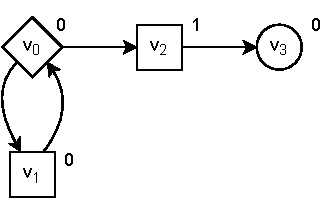
\includegraphics[scale=0.9]{Figs/inf-fixpoints-horiz.pdf}
\caption{Un juego con infinitos puntos fijos} \label{fig:multiple-fixpoints}
\end{figure}

\begin{example}\label{ex:several-fixpoints} Consideremos el juego (de un jugador) de la Figura~\ref{fig:multiple-fixpoints}, donde los vértices del Jugador $1$ están representados por cuadrados, los vértices del Jugador $2$ se muestran como rombos, los vértices probabilistas son círculos, y las recompensas son los números entre paréntesis. Observemos que, en este juego, el mayor punto fijo es $(1,1,1,0)$.  Sin embargo, $(\frac{1}{2},\frac{1}{2},1,0)$ también es un punto fijo ya que $\Gamma(\frac{1}{2},\frac{1}{2},1,0) = (\frac{1}{2},\frac{1}{2},1,0)$.  De hecho, el operador de Bellman para este juego tiene infinitos puntos fijos: cualquier $f$ de la forma $(x,x,1,0)$ con $x\in[0,1]$.
\end{example}

Por lo tanto, las técnicas tradicionales no aplican en este caso. En lugar de eso utilizamos el máximo punto fijo para probar determinación, pero esto no se puede realizar de forma directa usando $\StandardBellman$. Una dificultad principal es que el teorema de Knaspter-Tarski no se aplica a $\StandardBellman$ ya que $(\mathbb{R}^V, \leq)$ no es un retículo completo. Usando en su lugar los reales extendidos ($(\mathbb{R} \cup \{\infty\})^V$) no es una solución, ya que en algunos casos el punto fijo más grande asignará $\infty$ a algunos vértices (por ejemplo, $(\infty,\infty,0)$ sería el mayor punto fijo en la cadena de Markov de la Figura~\ref{fig:overflow}).
Un enfoque posible es aproximar el punto fijo más grande a partir de una cota superior estimada a través del algoritmo de \emph{value iteration}. Desafortunadamente, puede que no haya una relación de orden entre $f$ y $\StandardBellman(f)$ y puede resultar que para algún vértice $v$, $\StandardBellman(f)(v)>f(v)$ antes de converger al punto fijo. Esto se muestra en el siguiente ejemplo.

\begin{figure}
%\vspace{-6ex}
\centering
\scalebox{1.2}{
  \begin{tikzpicture}[on grid,auto,align at top]
    \node[minvert] (v0)                   {$v_0(10)$};
    \node[probvert] (v1) [right=2.3 of v0] {$v_1(0)$};
    \node[probvert] (v2) [right=2.3 of v1] {$v_2(0)$};
    
    \draw[rounded corners,->] (v0) -- (v1);
    \draw[rounded corners,->] (v1.east) -- ++(0,-1) node[pos=0.5] {$9/10$} -| (v0.south);
    \draw[rounded corners,->] (v1) -- (v2) node[midway] {$1/10$};   
  \end{tikzpicture}
  }
%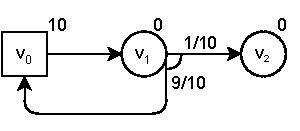
\includegraphics[scale=0.9]{Figs/overflow-horiz.pdf}
\caption{Un juego donde el valor puede aumentar.} \label{fig:overflow}
\end{figure}

\begin{example}\label{ex:overflow}
Consideremos el juego representado en la Figura~\ref{fig:overflow}.
El punto fijo (único) en este caso es $(100,90,0)$. Observemos que tenemos que $\StandardBellman(120,100,0) = (110, 108, 0)$, por lo que el valor en $v_1$ aumenta después de una iteración. Se necesitan varias iteraciones para alcanzar el mayor punto fijo. Por lo tanto, en general, la iteración del valor inicial desde un límite superior estimado no garantiza una convergencia monótona al punto fijo más grande.
\end{example}

Superamos los problemas antes mencionados usando una versión modificada de $\StandardBellman$. En términos generales, modificamos el operador Bellman de tal manera que opere sobre un retículo completo.

Observemos que, según el Lema~\ref{lm:memoryless-strat-p2-bounded-expectation}, el valor $\Expect{\strat{1}}{\strat{2}}_{\StochG,v}[\Rewards]$ es finito
para todo juego terminante bajo fairness $\StochG$ y estrategias $\strat{1} \in \DetMemorylessStrats{1}$, $\strat{2} \in \DetMemorylessFairStrats{2}$.
Además, debido a que la cantidad de estrategias deterministas sin memoria es finita, también tenemos que el número $\max \{ \inf_{\strat{2} \in \DetMemorylessFairStrats{2}} \sup_{\strat{1} \in \DetMemorylessStrats{1}} \Expect{\strat{1}}{\strat{ 2}}_{\StochG,v}[\Rewards] \mid v \in V \}$ está bien definido.
A partir de ahora, fijamos un número $\UpperBound \geq \max \{ \inf_{\strat{2} \in \DetMemorylessFairStrats{2}} \sup_{\strat{1} \in \DetMemorylessStrats{1}} \Expect {\strat{1}}{\strat{2}}_{\StochG,v}[\Rewards] \mid v \in V \}$. Definimos un operador de Bellman modificado $\Bellman: [0,\UpperBound]^V \rightarrow [0,\UpperBound]^V$ de la siguiente manera.
\[
    \Bellman(f)(v) =
    \begin{cases}
          \min \big( \reward(v) + \sum_{v' \in \post(v)} \delta(v,v')  f(v'),  \ \UpperBound \ \big ) &  \text{ si } v \in V_\Probabilistic \setminus T  \\
          \min\big( \max\{\reward(v)  + f(v') \mid v' \in \post(v) \}, \ \UpperBound  \ \big)& \text{ si } v \in  V_1 \setminus T, \\
          \min\big( \min\{\reward(v)  + f(v') \mid v' \in \post(v) \}, \ \UpperBound \ \big) & \text{ si } v \in  V_2 \setminus T, \\
           0 & \text{ si } v \in T.
    \end{cases}
\]
%% \[
%%     \Bellman(f)(v) =
%%     \begin{cases}
%%            \reward(v) + \sum_{v' \in \post(v)} \delta(v,v')  f(v') & \text{ if } v \in V_\Probabilistic  \\
%%           \min(\mathit{opt}_{\max}(f)(v), \mathbf{U} )& \text{ if } v \in  V_1 \setminus T, \\
%%           \min( \mathit{opt}_{\min}(f)(v), \textbf{U}) & \text{ if } v \in  V_2 \setminus T, \\
%%            0 & \text{ if } v \in T.
%%     \end{cases}
%% \]
%% where:
%% $
%%     \mathit{opt}_{\oplus}(f)(v) =  \oplus \{\reward(v)  + f(v') \mid v' \in \post(v) \}
%% $
%% and $\oplus \in \{\min, \max\}$.
%\[
%\mathit{opt}_{\min}(f)(v) =  \min \{\reward(v)  + f(v') \mid v' \in \post(v) \}.
%\]
Tengamos en cuenta que $\Bellman$ es monótona, lo que puede probarse observando que los máximos, mínimos y combinaciones convexas son todos operadores monótonos.
Además, $\Bellman$ también es \emph{Scott-continua} (conserva los supremos de los conjuntos dirigidos), esto se puede demostrar de manera similar a \cite{DBLP:conf/memics/BrazdilKN12}. La siguiente proposición
formaliza estas propiedades.
%\remarkPC{Podemos agregar una peque\~na discusion de por que la funci\'on tiene varios puntos fijo, quizas un ejemplo?}
\begin{proposition}\label{pn:continuity} $\Bellman$ es monótona y Scott-continua.
\end{proposition}

% PRUEBA PASADA AL APENDICE
\iffalse
\begin{proof}
    
    Primero, vamos a demostrar que $\Bellman$ es monótona. Consideremos $f,f' \in [0,\UpperBound]^V$  tal que
$f \leq f'$ por lo que $f(v) \leq f'(v')$ para todo $v \in V$.  La prueba es por casos:

    SI $v \in V_\Probabilistic$ y $\reward(v) + \sum_{v' \in \post(v)} \delta(v,v')* f(v') < \UpperBound$:
\begin{align}
    \Bellman(f)(v) & = \min (\reward(v) + \sum_{v' \in \post(v)} \delta(v,v')* f(v'), \UpperBound)\label{pn:continuity-eq1-l1} \\
            & \reward(v) + \sum_{v' \in \post(v)} \delta(v,v')* f(v') \label{pn:continuity-eq1-l2} \\
           & \leq \min (\reward(v) + \sum_{v' \in \post(v)} \delta(v,v') * f'(v'), \UpperBound)          \label{pn:continuity-eq1-l3} \\
           & = \Bellman(f')(v)  
\end{align}
    donde la linea \ref{pn:continuity-eq1-l3} se deduce por nuestras asunciones.
   
    Si $v \in V_\Probabilistic$ y $\reward(v) + \sum_{v' \in \post(v)} \delta(v,v')* f(v') \geq \UpperBound$, observemos que en este caso también $\reward(v) + \sum_{v' \in \post(v)} \delta(v,v')* f'(v') \geq \UpperBound$:
\begin{align}
    \Bellman(f)(v) & = \min(\reward(v) + \sum_{v' \in \post(v)} \delta(v,v')* f(v'), \UpperBound) \label{pn:continuity-eq2-l1} \\
                            & = \UpperBound                                                                  \label{pn:continuity-eq2-l2} \\
                            & = \min( \reward(v) + \sum_{v' \in \post(v)} \delta(v,v') * f'(v'), \UpperBound) \label{pn:continuity-eq2-l3} \\
                            & = \Bellman(f')(v)   \label{pn:continuity-eq2-l4}
\end{align}
donde las lineas \ref{pn:continuity-eq2-l2} y  \ref{pn:continuity-eq2-l3} son debido a la definición de $\Bellman$ y la asunción de $f \leq f'$.
    Los casos $v \in V_1$ y $v \in V_2$ son similares.
    
    La prueba de Scott-continuidad es como se detalla a continuación. Necesitamos probar que, para todo conjunto dirigido $D$, tenemos $\sup_{d \in D} \Bellman(d) =  \Bellman(\sup_{d \in D} d)$.
    La parte $\leq$ es directa por monotonía de $\Bellman$: $d \leq \sup_{d \in D} d$, entonces $\Bellman(d) \leq \Bellman( \sup_{d \in D} d)$ para todo $d$,
    por lo que, por propiedades de los supremos: $\sup_{d \in D} \Bellman(d) \leq  \Bellman(\sup_{d \in D} d)$.
    
    Probamos ahora la parte $\geq$.   Procedemos por cases:
    
    Si   $v \in V_1$,  entonces:
     \begin{align}
     \Bellman (\sup_{d \in D} d)(v) & = \min ( \max \{ \reward(v) + (\sup_{d \in D} d)(v') \mid v' \in \post(v)\},  \UpperBound ) \\                                                                                       
                                                     & =\min(  \sup_{d \in D} ( \max \{\reward(v) + d(v') \mid v' \in \post(v) \}, \UpperBound ) \\
                                                     & = \sup_{d \in D} (\min( \max \{ \reward(v) + d(v') \mid v' \in \post(v) \}, \UpperBound)) \\
                                                     & =  \sup_{d \in D} \Bellman(d)
    \end{align}
    
    Si $v \in V_2$  y $\min \{ \reward(v) + (\sup_{d \in D} d)(v') \mid v' \in \post(v)\} > \UpperBound$. Por lo que, para
    cualquier $v' \in \post(v)$ tenemos  $\reward(v) + (\sup_{d \in D} d)(v') > \UpperBound$, o equivalentemente: 
    $\sup_{d \in D} (\reward(v) + d(v')) > \UpperBound$. Entonces, para todo $v' \in \post(v)$ existe algún $d \in D$: $(\reward(v) + d(v')) > \UpperBound$.
    Por lo tanto, como $D$ es dirigido tenemos un $d^* \in D$ tal que para todo $v' \in \post(v)$: $(\reward(v) + d^*(v')) > \UpperBound$, entonces 
    $\sup_{d \in D} \min ( \min \{ \reward(v) + d(v') \mid v' \in \post(v)\}, \UpperBound) = \UpperBound$.
     
     Si $v \in V_2$  y $\min \{ \reward(v) + (\sup_{d \in D} d)(v') \mid v' \in \post(v)\} < \UpperBound$.  Tenemos que
     $\Bellman((\Sup_{d \in D} d) v) = \min \{ \reward(v) + (\sup_{d \in D} d)(v') \mid v' \in \post(v)\}$. En aras de la contradicción asumamos que $\Bellman((\Sup_{d \in D} d)(v)) > \sup_{d \in D} \Bellman(d)(v)$, lo que implica que
    $\min \{ \reward(v) + (\sup_{d \in D} d)(v') \mid v' \in \post(v)\} > \sup_{d \in D} \Bellman(d)(v)$. Esto implica
    que para todo $v' \in \post(v)$ existe un $d \in D$ tal que  $\reward(v) + d(v')  > \sup_{d \in D} \Bellman(d)(v)$.
    Como $D$ es dirigido esto significa que existe un $d^* \in D$ tal que para todo $v' \in \post(v)$: $\reward(v) + d^*(v')  > \sup_{d \in D} \Bellman(d)(v)$,
    por lo tanto $\min \{ \reward(v) + d^*(v') \mid v' \in \post(v)  \} > \sup_{d \in D} \Bellman(d)(v)$, o equivalentemente:
    $\min \{ \reward(v) + d^*(v') \mid v' \in \post(v)  \} > \sup_{d \in D} \min \{ \reward(v) + d(v') \mid v' \in \post(v)\}$ lo cual es una contradicción ya que $d^* \in D$.
     
    Para $v \in V_\Probabilistic$ la prueba es similar al caso de $v \in V_1$.\qedhere
\end{proof}
\fi

Observemos que $([0,\UpperBound]^V, \leq)$ es un retículo completo. Por lo tanto, por la Proposición \ref{pn:continuity} y el teorema de Knaster-Tarski \cite{davey1990introduction}., el conjunto (no vacío) de puntos fijos de $\Bellman$ forman un retículo completo, y el punto fijo mayor del operador puede ser aproximado por las aplicaciones sucesivas de $\Bellman$ al elemento tope (es decir, $\UpperBound$) \cite{davey1990introduction}. A partir de aquí denotaremos por $\nu \Bellman$ al mayor punto fijo de $\Bellman$.

%The following theorem states that game determinacy is preserved when Player 2 is restricted to play fair strategies.
El teorema que se da a continuación establece que los juegos restringidos a estrategias \textit{fair} sobre el Jugador $2$ están determinados.
Además, el valor del juego está dado por el máximo punto fijo de $\Bellman$.
\begin{theorem}\label{thm:game-determinacy} Sea $\StochG$ un juego estocástico que es terminante bajo \textit{fairness}. Se satisface que:
\[\adjustlimits
	\inf_{\strat{2} \in \FairStrats{2}} \sup_{\strat{1} \in \Strategies{1}} \Expect{\strat{1}}{\strat{2}}_{\StochG,v}[\Rewards] = \adjustlimits \sup_{\strat{1} \in \Strategies{1}}   \inf_{\strat{2} \in \FairStrats{2}}  \Expect{\strat{1}}{\strat{2}}_{\StochG,v}[\Rewards] = \nu \Bellman(v)
\]
\end{theorem}
%
\begin{proof}
  Primero, observemos que $\inf_{\strat{2} \in \DetMemorylessFairStrats{2}}  \sup_{\strat{1} \in \DetMemorylessStrats{1}} \Expect{\strat{1}}{\strat{2}}_{\StochG,v}[\Rewards]$
  es un punto fijo de $\Bellman$.  Por lo que tenemos:
   \begin{align*}	
       % \label{thm:game-determinacy-eq1-l1}
        \adjustlimits \sup_{\strat{1} \in \Strategies{1}}   \inf_{\strat{2} \in \FairStrats{2}}  \Expect{\strat{1}}{\strat{2}}_{\StochG,v}[\Rewards]
        & \leq \adjustlimits \inf_{\strat{2} \in \FairStrats{2}} \sup_{\strat{1} \in \Strategies{1}} \Expect{\strat{1}}{\strat{2}}_{\StochG,v}[\Rewards] \\
      % \label{thm:game-determinacy-e1-l2}
        &   \leq \adjustlimits  \inf_{\strat{2} \in \DetMemorylessFairStrats{2}}  \sup_{\strat{1} \in \DetMemorylessStrats{1}} \Expect{\strat{1}}{\strat{2}}_{\StochG,v}[\Rewards] 
         \leq   \nu \Bellman(v) 
  \end{align*} 
  %First, note that $\inf_{\strat{2} \in \FairStrats{2}} \sup_{\strat{1} \in \Strategies{1}} \Expect{\strat{1}}{\strat{2}}_{\StochG,v}[\Rewards]$ is a fixed point of $\Gamma$. 
  %Thus we have:
  %\[
  %\adjustlimits
  %\sup_{\strat{1} \in \Strategies{1}}   \inf_{\strat{2} \in \FairStrats{2}}  \Expect{\strat{1}}{\strat{2}}_{\StochG,v}[\Rewards]
  %\leq 
  %\adjustlimits \inf_{\strat{2} \in \FairStrats{2}} \sup_{\strat{1} \in \Strategies{1}} \Expect{\strat{1}}{\strat{2}}_{\StochG,v}[\Rewards]
  %\leq
  %\inf_{\strat{2} \in \DetMemorylessFairStrats{2}}  \sup_{\strat{1} \in \DetMemorylessStrats{1}} \Expect{\strat{1}}{\strat{2}}_{\StochG,v}[\Rewards]
  %\leq
  %\nu \Gamma(v)
  %\]
  para cualquier $v$. La primer desigualdad es una propiedad estándar de los supremos e ínfimos \cite{Kucera2011}, la segunda desigualdad vale por
  $\DetMemorylessFairStrats{2} \subseteq \FairStrats{2}$  y propiedades estándar sobre MDPs: al fijar una estrategia \textit{fair} determinista sin memoria para el Jugador $2$ obtenemos un MDP transitorio, la estrategia óptima para el Jugador $1$ en este MDP se obtiene por medio de una estrategia determinista sin memoria \cite{Kallenberg83}. La última desigualdad se cumple ya que  $\inf_{\strat{2} \in \DetMemorylessFairStrats{2}}  \sup_{\strat{1} \in \DetMemorylessStrats{1}} \Expect{\strat{1}}{\strat{2}}_{\StochG,v}[\Rewards]$ es 
  un punto fijo de $\Bellman$. 
  
  Queda probar que $\sup_{\strat{1} \in \Strategies{1}}   \inf_{\strat{2} \in \FairStrats{2}}  \Expect{\strat{1}}{\strat{2}}_{\StochG,v}[\Rewards] \geq \nu \Bellman(v)$. Observemos que, si existe  $\strat{1} \in \Strategies{1}$ tal que
  $\inf_{\strat{2} \in \FairStrats{2}}  \Expect{\strat{1}}{\strat{2}}_{\StochG,v}[\Rewards] \geq \nu \Bellman(v)$ la propiedad de arriba se deduce por propiedades de los supremos. Consideremos la estrategia $\starredstrat{1}$ definida de la siguiente manera:
  $\starredstrat{1}(v) \in \argmax \{\nu \Bellman(v') + \reward(v) \mid v' \in \post(v) \}$. Notemos que $\starredstrat{1}$ es una estrategia determinista sin memoria. Para cualquier estrategia determinista, sin memoria y fair $\strat{2} \in \DetMemorylessFairStrats{2}$ tenemos
  $\nu \Bellman(v) \leq \Expect{\starredstrat{1}}{\strat{2}}_{\StochG,v}[\Rewards]$ (por definición de $\Bellman$).  Por lo tanto,
  %
  $\nu \Bellman(v) \leq \inf_{\strat{2} \in \DetMemorylessFairStrats{2}} \Expect{\starredstrat{1}}{\strat{2}}_{\StochG,v}[\Rewards]$
  %
  y en consecuencia:
  %
  $\nu \Bellman(v) \leq \sup_{\strat{1} \in \DetMemorylessStrats{1}} \inf_{\strat{2} \in \DetMemorylessFairStrats{1}} \Expect{\strat{1}}{\strat{2}}_{\StochG,v}[\Rewards]$.
  %
  Finalmente, por el Teorema~\ref{thm:reduce-to-memoryless} obtenemos:
  %
  $\nu \Bellman(v) \leq \sup_{\strat{1} \in \Strategies{1}} \inf_{\strat{2} \in \FairStrats{2}} \Expect{\strat{1}}{\strat{2}}_{\StochG,v}[\Rewards]$.
  \qedhere
\end{proof}
%
%\subsection{Considerations for an algorithmic solution}
\subsection{Consideraciones para una solución algorítmica.} 
El algoritmo de \emph{value iteration} \cite{Bellman57} se ha utilizado para calcular la recompensa acumulada esperada máxima/mínima en procesos de decisión de Markov, por ejemplo, en el \textit{model checker} {\Prism}. Por lo general, el valor se calcula aproximando el punto fijo mínimo desde abajo utilizando las ecuaciones de Bellman \cite{Bellman57}. En~\cite{DBLP:conf/cav/Baier0L0W17}, los autores proponen acercarse a estos valores desde un límite superior e inferior (conocido como \emph{interval iteration} \cite{DBLP:journals/tcs/HaddadM18}). Para hacerlo, \cite{DBLP:conf/cav/Baier0L0W17} muestra una técnica para calcular las cotas superiores de las recompensas totales esperadas para los MDPs. Este enfoque se basa en el hecho de que, dado un MDP terminante $\StochG$, $\ExpectMDP{\strat{1}}_{\mathcal{G},v}[\Rewards] = \sum_{v' \in R(v)} \zeta_v^{\strat{1}}(v')*\reward(v')$, donde $R(v)$ denota el conjunto de estados alcanzables desde $v$, y $\zeta_v ^{\strat{1}}(v')$ denota el número esperado de veces que se visita $v'$ en la cadena de Markov inducida por $\strat{1}$ cuando comienza en $v$. \cite{DBLP:conf/cav/Baier0L0W17} describe cómo calcular un valor $\zeta_{v}^*(v')$, tal que $\zeta_v^*(v') \geq \sup_{\strat{ 1} \in \Strategies{1}} \zeta_v^{\strat{1}}(v')$. Por lo tanto, $\sum_{v' \in R(v)} \zeta_v^{*}(v')*\reward(v')$ da un límite superior para $\sup_{\strat{1}} \ExpectMDP {\strat{1}}_{\mathcal{G},v}[\Rewards]$.

\begin{figure}
    \centering
    %\vspace{-9.5ex}
    \begin{minipage}{0.75\textwidth}
      \begin{algorithm}[H]
      \SetAlgoLined
      \KwIn{Juego estocástico $\StochG = \langle V, (V_1, V_2,V_\Probabilistic),\delta \rangle$}
      \KwOut{$\nu \Bellman$}
        \caption{Algoritmo para computar el máximo punto fijo}\label{Alg:gfp}
        \begin{algorithmic}
          \REQUIRE $\StochG$ es un juego terminante bajo \textit{fairness}\\[1ex]
          \STATE $\delta' \gets  \lambda (v,v') {.} (v \in V_1 {\cup} V_\Probabilistic) \mathop{?} \delta(v,v') : \frac{1}{|\post^{\mathcal{G}}(v)|}$\\[-1ex]
          \STATE  $\mathcal{G}' \gets (V, (V_1, \emptyset, V_2{\cup}V_\Probabilistic)), \delta')$
          \STATE $x' \gets \lambda v : \sum_{v' \in R(v)} : \zeta^*_v(v')*\reward(v')$
          \REPEAT
          \STATE $x \gets x'$
          \STATE $x' \gets \Bellman(x)$
          \UNTIL{$|| x - x' || \leq \varepsilon$}
          \RETURN $x'$
        \end{algorithmic}
      \end{algorithm}
    \end{minipage}
  \end{figure}
    Nuestro algoritmo utiliza estas ideas para proporcionar una cota superior para los juegos de dos jugadores. En términos generales, el funcional $\Bellman$ definido anteriormente presenta una forma de ecuaciones de Bellman que permite que un algoritmo de \emph{value iteration} resuelva estos juegos. Necesitamos comenzar con un vector de valores más grande que dicho punto fijo. Dado un juego terminante bajo \textit{fairness}, fijamos una estrategia \textit{fair} (sin memoria) para el ambiente, obteniendo así un MDP. Luego usamos las técnicas descritas anteriormente para encontrar un límite superior para este MDP, que a su vez es una cota superior en el juego original. La estrategia \textit{fair} obvia a usar es la que se basa en la distribución uniforme (como en el Teorema \ref{thm:uniform-prob}). Esta idea se describe en Algoritmo~\ref{Alg:gfp}. Vale la pena señalar que, en lugar de usar un límite superior único para cada vértice (como en la definición de $\Bellman$), el algoritmo puede usar un límite superior diferente para cada componente del vector de valores, lo que mejora el número de iteraciones realizada por el algoritmo.
Hemos implementado el Algoritmo~\ref{Alg:gfp} como un prototipo embebido en el conjunto de herramientas {\PrismGames} ~\cite{DBLP:conf/cav/KwiatkowskaN0S20}, 
como se describe en la próxima sección. 
%\remarkPC{Agregar un parrafo que en vez de usar $\UpperBound$, usamos un vector.}
%\remarkPRD{Por ah\'i yo dir\'ia \textbf{``We have implemented this algorithm as a prototype embedded in the {\Prism}-game toolset~\cite{DBLP:conf/cav/KwiatkowskaN0S20}.''} De cualquier manera, el paper \cite{DBLP:conf/cav/KwiatkowskaN0S20}. hay que referenciarlo }
   %    We have implemented these ideas in a prototype tool as described in the next section.


%% old text
%Value iteration \cite{Bellman57} has been used to compute maximum/minimum expected accumulated reward in MDPs, e.g. in the {\Prism} model checker.  Usually, the value is computed by approximating the least fixed point from below using the Bellman equations \cite{Bellman57}. In~\cite{DBLP:conf/cav/Baier0L0W17}, the authors propose to approach these values from both a lower and an upper bound (known as interval iteration \cite{DBLP:journals/tcs/HaddadM18}). To do so,  \cite{DBLP:conf/cav/Baier0L0W17} shows a technique for computing upper bounds for the expected total rewards for MDPs.

%The above defined functional $\Bellman$ presents a form of Bellman equations that enables a value iteration algorithm to solve our games.  As we are looking for the greatest fixed point, we need to start with some value vector larger than such a fixed point.
%
%If we take our game and fix a fair strategy for the environment, we obtain an MDP. We can then use the techniques presented in \cite{DBLP:conf/cav/Baier0L0W17} to find an upper bound in this MDP, which in turn is an upper bound in the original game. The obvious fair strategy to use is the one based on the uniform distribution (as in Theorem \ref{thm:uniform-prob}).  We have implemented these ideas in a prototype tool as described in the next section.

\section{Validación Experimental} \label{sec:experimental_eval_fair}

\definecolor{Gray}{gray}{0.9}
\definecolor{Gray2}{gray}{0.95}
\newcolumntype{g}{>{\columncolor{Gray}}c}
\newcolumntype{h}{>{\columncolor{Gray2}}c}

Para evaluar la viabilidad de nuestro enfoque, hemos ampliado sobre el model checker {\Prism}~\cite{DBLP:conf/cav/KwiatkowskaN0S20,DBLP:conf/cav/KwiatkowskaNP11} con un operador para calcular las recompensas esperadas de los juegos estocásticos terminantes bajo fairness. El prototipo de esta herramienta también permite verificar si un juego se detiene bajo fairness.
%implementó una herramienta prototipo llamada \textsf{SynthFairy} (disponible en \cite{SynthFairy})
% y ejecútelo en dos conjuntos diferentes de ejemplos. %\footnote{Disponible en \cite{SynthFairy}}.
La herramienta toma como entrada un modelo que describe el juego en notación {\Prism} y devuelve como salida
la recompensa total esperada óptima para un estado inicial dado, así como la estrategia de controlador óptima sintetizada (bajo supuestos de fairness sobre el ambiente).
%Los modelos de entrada se especifican usando un lenguaje parecido a la notación {\Prism} \cite{DBLP:conf/cav/KwiatkowskaNP11}.
La evaluación experimental muestra que nuestro enfoque puede hacer frente a casos de estudio no triviales. Para calcular estos valores establecemos un error relativo de como máximo $\varepsilon = 10^{-6}$.


%We have considered variations of two examples:
%For the model presented in Sec.~\ref{sec:mot_example}, the expected total reward when $\verb"P"=0.1$ and $\verb"Q"=0$ is $5.55$. Moreover, 
%the non-trivial part of the synthesized strategy is illustrated with the black arrows in Fig.~\ref{fig:robot_game_grid}.
\paragraph{Roborta vs. la Luz fair.}
Consideramos tres variantes del caso de estudio: versión A (la luz no falla), versión B (la luz solo puede fallar cuando intenta dar una luz verde) y versión C (la luz puede fallar cuando intenta activar cualquier tipo de luz).
Asumimos que, cuando Roborta falla, esta no puede moverse (esto es beneficioso para Roborta ya que nuevamente puede recolectar la recompensa asignada a esa posición);
cuando falla la luz, el robot puede moverse libremente en cualquier dirección permitida.
La configuración de la matriz (restricciones de movimiento y recompensas) se genera aleatoriamente. Para cada configuración, la Tabla~\ref{table:resultsRobot} describe los resultados para tres escenarios diferentes generados a partir de semillas diferentes. La primera columna describe el tamaño de la matriz. La segunda columna indica la probabilidad de falla del robot ($P$) y la luz ($Q$).
Las otras columnas describen el tamaño del modelo, la recompensa total esperada para la estrategia óptima y el número de iteraciones realizadas, respectivamente para tres configuraciones diferentes generadas aleatoriamente.
Para la configuración de matriz que se muestra en Sección~\ref{sec:mot_example_fair} con parámetros $P=0.1$ y $Q=0$, la herramienta derivó la estrategia óptima representada en la Figura~\ref{fig:robot_game_grid} e informa una recompensa total esperada de $5.55$.


%We explain Table~\ref{table:resultsRobot} with an example.  Take the case of the grid $A \mid {60{\times}8} \mid \text{seed } 1$, with the robot fault probability being $0.1$, the optimal expected total reward is $26.66$ and the number of decisions made by the robot when both players play optimally is $2$.  We consider a decision as a choice resolution introduced when the yellow light is on on a cell without movement restrictions or if the light is off. We use this number to give us an idea that resolutions are not trivial, and to hint a different resolution for closely related instances.
%Indeed, notice that for the case mentioned above, when the fault probability is set to $0.9$ (instead of $0.1$), the number of decisions changes to $0$. 
%This suggests that the strategy of the environment for lower fault probabilities was not worth it anymore, thereby it finds a better strategy. 

\begin{table}[tp]
  \centering\noindent%
  %\vspace{-0.5cm}
  %\vspace{-0.8cm}
  \scalebox{0.72}{
    \small
    \renewcommand{\arraystretch}{1.5}%
    \begin{tabular}{c|c|c|c|c|c|c|c|c|c|c|c}
      
      \multirow{2}{*}{Versión} & \multicolumn{2}{c|}{Prob.Falla} & \multicolumn{3}{c|}{Tamaño (Estados/Transiciones)} & \multicolumn{3}{c|}{Rec.\ Total.\ Esp. Opt.} & \multicolumn{3}{c}{Iteraciones}\\ \hhline{|~|-|-|-|-|-|-|-|-|-|-|-|}
      & $P$ & $Q$ &  s.\ 1 & s.\ 2 & s.\ 3 & \makebox[3.4em][c]{s.\ 1} & \makebox[3.4em][c]{s.\ 2} & \makebox[3.4em][c]{s.\ 3} & \makebox[1.8em][c]{s.\ 1} & \makebox[1.8em][c]{s.\ 2} & \makebox[1.8em][c]{s.\ 3}  \\  
      \hline
       \multirow{2}{3em}{\centering $A$ \\ $60{\times}8$}
       & $0.1$ & $-$ & \multirow{2}{*}{\centering $\displaystyle \begin{array}{c} \text{st. }1448 \\ \text{tr. }3220 \end{array}$} & \multirow{2}{*}{\centering $\displaystyle \begin{array}{c} \text{st. }1418 \\ \text{tr. }3112 \end{array}$}  & \multirow{2}{*}{\centering $\displaystyle \begin{array}{c} \text{st. }1421 \\ \text{tr. }3132 \end{array}$}  & $26.66$ & $31.11$ & $27.77$ & $711$ & $681$ & $252$\\ \hhline{|~|-|-|~|~|~|-|-|-|-|-|-|}
       & $0.5$ & $-$ & & & & $48$ & $56$ & $50$ & $2253$ & $2225$ & $475$\\ \hline

       \multirow{2}{3em}{\centering $A$ \\ $120{\times}16$}
       & $0.1$ & $-$ & \multirow{2}{*}{\centering $\displaystyle \begin{array}{c} \text{st. }5686 \\ \text{tr. }12586 \end{array}$} & \multirow{2}{*}{\centering $\displaystyle \begin{array}{c} \text{st. }5716 \\ \text{tr. }12658 \end{array}$}  & \multirow{2}{*}{\centering $\displaystyle \begin{array}{c} \text{st. }5716 \\ \text{tr. }12722 \end{array}$}  & $62.22$ & $55.55$ & $48.88$ & $687$ & $700$ & $685$ \\ \hhline{|~|-|-|~|~|~|-|-|-|-|-|-|}
       & $0.5$ & $-$ & & & & $112$ & $100$ & $88$ & $2231$ & $2265$ & $2229$ \\ \hline

       \multirow{4}{3em}{\centering $B$ \\ $60{\times}8$}
       & \multirow{2}{*}{$0.1$} & $0.1$ & \multirow{4}{*}{\centering $\displaystyle \begin{array}{c} \text{st. }1928 \\ \text{tr. }5952 \end{array}$} & \multirow{4}{*}{\centering $\displaystyle \begin{array}{c} \text{st. }1888 \\ \text{tr. }5746 \end{array}$}  & \multirow{4}{*}{\centering $\displaystyle \begin{array}{c} \text{st. }1892 \\ \text{tr. }5785 \end{array}$}  & $42.6$ & $44.59$ & $42.23$ & $479$ & $335$ & $388$ \\ \hhline{|~|~|-|~|~|~|-|-|-|-|-|-|}
       & & $0.5$ & & & & $130.14$ & $127.7$ & $136.22$ & $772$ & $689$ & $824$ \\ \hhline{|~|-|-|~|~|~|-|-|-|-|-|-|}
       & \multirow{2}{*}{$0.5$} & $0.1$ & & & & $76.68$ & $80.26$ & $76.02$ & $873$ & $764$ & $909$ \\ \hhline{|~|~|-|~|~|~|-|-|-|-|-|-|}
       & & $0.5$ & & & & $234.26$ & $229.87$ & $245.21$ & $1263$ & $1139$ & $1341$ \\ \hline

       \multirow{4}{3em}{\centering $B$ \\ $120{\times}16$}
       & \multirow{2}{*}{$0.1$} & $0.1$ & \multirow{4}{*}{\centering $\displaystyle \begin{array}{c} \text{st. }7576 \\ \text{tr. }23266 \end{array}$} & \multirow{4}{*}{\centering $\displaystyle \begin{array}{c} \text{st. }7616 \\ \text{tr. }23400 \end{array}$}  & \multirow{4}{*}{\centering $\displaystyle \begin{array}{c} \text{st. }7616 \\ \text{tr. }23528 \end{array}$}  & $91.19$ & $87.27$ & $80.07$ & $538$ & $544$ & $616$ \\ \hhline{|~|~|-|~|~|~|-|-|-|-|-|-|}
       & & $0.5$ & & & & $281.83$ & $281.48$ & $265.33$ & $1076$ & $1118$ & $1252$\\ \hhline{|~|-|-|~|~|~|-|-|-|-|-|-|}
       & \multirow{2}{*}{$0.5$} & $0.1$ & & & & $164.15$ & $157.1$ & $144.13$ & $1147$ & $1223$ & $1373$ \\ \hhline{|~|~|-|~|~|~|-|-|-|-|-|-|}
       & & $0.5$ & & & & $507.30$ & $506.67$ & $477.6$ & $1850$ & $1865$ & $2088$ \\ \hline

       \multirow{4}{3em}{\centering $C$ \\ $60{\times}8$}
       & \multirow{2}{*}{$0.1$} & $0.1$ & \multirow{4}{*}{\centering $\displaystyle \begin{array}{c} \text{st. }1928 \\ \text{tr. }6432 \end{array}$} & \multirow{4}{*}{\centering $\displaystyle \begin{array}{c} \text{st. }1888 \\ \text{tr. }6216 \end{array}$}  & \multirow{4}{*}{\centering $\displaystyle \begin{array}{c} \text{st. }1892 \\ \text{tr. }6256 \end{array}$}  & $46.32$ & $47.07$ & $44.87$ & $379$ & $336$ & $390$ \\ \hhline{|~|~|-|~|~|~|-|-|-|-|-|-|}
       & & $0.5$ & & & & $143.35$ & $146.41$ & $153.98$ & $742$ & $658$ & $774$ \\ \hhline{|~|-|-|~|~|~|-|-|-|-|-|-|}
       & \multirow{2}{*}{$0.5$} & $0.1$ & & & & $83.37$ & $84.73$ & $80.77$ & $879$ & $769$ & $914$ \\ \hhline{|~|~|-|~|~|~|-|-|-|-|-|-|}
       & & $0.5$ & & & & $258.04$ & $263.53$ & $277.17$ & $1202$ & $1076$ & $1246$ \\ \hline

       \multirow{4}{3em}{\centering $C$ \\ $120{\times}16$}
       & \multirow{2}{*}{$0.1$} & $0.1$ & \multirow{4}{*}{\centering $\displaystyle \begin{array}{c} \text{st. }7576 \\ \text{tr. }25156 \end{array}$} & \multirow{4}{*}{\centering $\displaystyle \begin{array}{c} \text{st. }7616 \\ \text{tr. }25300 \end{array}$}  & \multirow{4}{*}{\centering $\displaystyle \begin{array}{c} \text{st. }7616 \\ \text{tr. }25428 \end{array}$}  & $98.25$ & $93.74$ & $88.33$ & $533$ & $544$ & $606$ \\ \hhline{|~|~|-|~|~|~|-|-|-|-|-|-|}
       & & $0.5$ & & & & $321.18$ & $317.61$ & $311.62$ & $1002$ & $1068$ & $1188$ \\ \hhline{|~|-|-|~|~|~|-|-|-|-|-|-|}
       & \multirow{2}{*}{$0.5$} & $0.1$ & & & & $176.85$ & $168.73$ & $158.99$ & $1147$ & $1227$ & $1365$\\ \hhline{|~|~|-|~|~|~|-|-|-|-|-|-|}
       & & $0.5$ & & & & $578.13$ & $571.71$ & $560.92$ & $1700$ & $1760$ & $1956$ \\ 

      \hline
    \end{tabular}
  }
  \caption{Resultados del juego Roborta vs. la Luz fair.}
  \label{table:resultsRobot}
  %\vspace{-0.8cm}
\end{table}


% Figure follows ------------------
\begin{figure}
%\vspace{-10mm}
%\vspace{-11mm}
%\fontsize{6.6}{6.6}\selectfont\ttfamily
\centering
\scalebox{1.0}{
  \begin{tikzpicture}[on grid,auto,align at top]
    \node[draw,fill=white,circle,thick,align=center,inner sep=3pt,minimum size=7mm] (v0)                   {$w_0(1,1,1)$};
    \node[draw,fill=pink,circle,thick,align=center,inner sep=3pt,minimum size=7mm] (v1) [right=3 of v0]                  {$w_1(1,3,3)$};
    \node[draw,fill=white,circle,thick,align=center,inner sep=3pt,minimum size=7mm] (v2) [above=2 of v1]                   {$w_2(1,1,1)$};
    \node[draw,fill=white,circle,thick,align=center,inner sep=3pt,minimum size=7mm] (v3) [above=2 of v2]                  {$w_3(1,1,1)$};
    \node[draw,fill=pink,circle,thick,align=center,inner sep=3pt,minimum size=7mm] (v4) [left=3 of v3]                  {$w_4(1,1,2)$};
    \node[draw,fill=pink,circle,thick,align=center,inner sep=3pt,minimum size=7mm] (v5) [above=2 of v0]              {$w_5(1,4,4)$};
    
    \draw (v0) -- (v1);
    \draw (v1) -- (v2);
    \draw (v2) -- (v3);
    \draw (v3) -- (v4);
    \draw (v4) -- (v5);
    \draw (v4) -- (v1);
    \draw[red,dashed] (v5) -- (v1);
    \draw (v5) -- (v0);
  \end{tikzpicture}
  }
%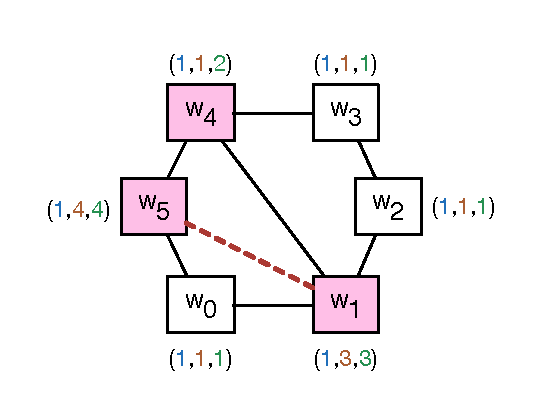
\includegraphics[scale=0.80]{Figs/uav.eps}
%\vspace{-10mm}
\caption{Red UAV para misiones ISR} \label{fig:uav_game_map}
%\caption{A robot game on a $4 \times 4$ grid starting on location (0,0). Each location has an assigned positive reward. The sideway movement restrictions are depicted as white arrows on the bottom-right of each location. The best strategy for the robot when the light is yellow is shown in black arrows on the top-right of the locations without movement restrictions. The path taken by the robot to achieve the goal is highlighted in yellow} \label{fig:robot_game_grid}
\end{figure}
%
\paragraph{UAV autónomo vs. Operador humano.} Adaptamos el caso de estudio analizado en \cite{DBLP:conf/iccps/FengWHT15}. Se utiliza un vehículo aéreo no tripulado (UAV) controlado a distancia para realizar misiones de inteligencia, vigilancia y reconocimiento (ISR) en una red de carreteras. El UAV realiza funciones de pilotaje de forma autónoma (seleccionando una ruta para volar entre \emph{puntos de referencia}). El operador humano (entorno) controla el sensor a bordo para capturar imágenes en un punto de referencia, así como las funciones de pilotaje en ciertos puntos de referencia (llamados puntos de control). Tengamos en cuenta que un operador puede tratar continuamente de obtener una mejor imagen haciendo que el UAV merodee alrededor de un determinado punto de referencia, lo que puede conducir a un comportamiento unfair.
%Asignamos recompensas a una captura exitosa de un waypoint no visitado.
Cada captura exitosa de un punto de referencia no visitado otorga una recompensa.

%
La Figura~\ref{fig:uav_game_map} muestra un ejemplo de red de carreteras que consta de seis puntos de referencia de vigilancia etiquetados $w_0,w_2,...,w_5$, los arcos representan rutas de conexión, una línea discontinua roja significa que la ruta es lo suficientemente peligrosa como para hacer que el UAV deje de funcionar con una probabilidad de $1$, mientras que en cualquier otro camino, esta probabilidad es de $S$. Los puntos de control se representan como nodos rosas, en los que el operador aún puede delegar la tarea de pilotaje al UAV con probabilidad $D$. Cada nodo está anotado con tres posibles recompensas. Por ejemplo, para $S=0.3$ y $D=0.5$ y los valores de recompensa más a la izquierda en cada terna, la estrategia sintetizada para el UAV intenta seguir el circuito óptimo $w_0,w_1,w_2,w_3,w_4,w_5$. Mientras que para los valores de recompensa del medio y más a la derecha, los circuitos óptimos a seguir son $w_0,w_5,w_0,w_1,w_2,w_3,w_4$ y $w_0,w_5,w_4,w_1,w_2,w_3$, respectivamente. 
La Tabla~\ref{table:resultsUAV} muestra los resultados obtenidos para este juego para varias redes de carreteras generadas aleatoriamente. La primera columna describe el número de puntos de referencia utilizados. La segunda columna indica la probabilidad de delegación ($D$) y la probabilidad de que el UAV deje de funcionar ($S$).
Las otras columnas muestran el tamaño del modelo, la recompensa total esperada para la estrategia óptima y el número de iteraciones realizadas, respectivamente, para tres configuraciones diferentes de mapas de ruta generadas aleatoriamente.

Las tablas~\ref{table:resultsRobot} y~\ref{table:resultsUAV} no informan el tiempo necesario para calcular los resultados, pero en todos los casos la salida se calculó en menos de 400 segundos. Todos los experimentos se realizaron en un MacBook Air con Intel Core i5 a 1,3 GHz y 4 GB de RAM. Tanto la herramienta como los casos de estudio se encuentran disponibles en un repositorio github~\cite{FairPrism}.

\begin{table}[ht]
  \centering\noindent%
  %\vspace{-0.5cm}
  %\vspace{-0.8cm}
  \scalebox{0.72}{
    \small
    \renewcommand{\arraystretch}{1.5}%
    \begin{tabular}{c|c|c|c|c|c|c|c|c|c|c|c}
      
      \multirow{2}{*}{Versión} & \multicolumn{2}{c|}{Prob.} & \multicolumn{3}{c|}{Tamaño(Estados/Transiciones)} & \multicolumn{3}{c|}{Rec.\ Total.\ Esp. Opt.} & \multicolumn{3}{c}{Iteraciones} \\ \hhline{|~|-|-|-|-|-|-|-|-|-|-|-|}
      & $D$ & $S$ & s.\ 1 & s.\ 2 & s.\ 3 & {s.\ 1} & {s.\ 2} & {s.\ 3} & {s.\ 1} & {s.\ 2} & {s.\ 3} \\  
      \hline
       \multirow{4}{3em}{\centering UAV \\ $6w.$}
       & \multirow{2}{*}{$0.1$} & $0.05$ & \multirow{4}{*}{\centering $\displaystyle \begin{array}{c} \text{st. }213 \\ \text{tr. }504 \end{array}$} & \multirow{4}{*}{\centering $\displaystyle \begin{array}{c} \text{st. }508 \\ \text{tr. }1368 \end{array}$} & \multirow{4}{*}{\centering $\displaystyle \begin{array}{c} \text{st. }136 \\ \text{tr. }312 \end{array}$} & $16.72$ & $12.47$ & $13.14$ & $142$ & $248$ & $22$ \\ \hhline{|~|~|-|~|~|~|-|-|-|-|-|-|}
       & & $0.1$ & & & & $15.73$ & $11.15$ & $12.63$ & $73$ & $188$ & $22$ \\ \hhline{|~|-|-|~|~|~|-|-|-|-|-|-|}
       & \multirow{2}{*}{$0.5$} & $0.05$ & & & & $20.49$ & $12.77$ & $17.05$ & $103$ & $133$ & $22$ \\ \hhline{|~|~|-|~|~|~|-|-|-|-|-|-|}
       & & $0.1$ & & & & $18.87$ & $11.67$ & $15.95$ & $55$ & $70$ & $22$ \\ \hline

       \multirow{4}{3em}{\centering UAV \\ $8w.$}
       & \multirow{2}{*}{$0.1$} & $0.05$ & \multirow{4}{*}{\centering $\displaystyle \begin{array}{c} \text{st. }2177 \\ \text{tr. }5959 \end{array}$} & \multirow{4}{*}{\centering $\displaystyle \begin{array}{c} \text{st. }3591 \\ \text{tr. }9991 \end{array}$} & \multirow{4}{*}{\centering $\displaystyle \begin{array}{c} \text{st. }1426 \\ \text{tr. }3604 \end{array}$} & $17.88$ & $40.59$ & $24.6$ & $407$ & $332$ & $779$ \\ \hhline{|~|~|-|~|~|~|-|-|-|-|-|-|}
       & & $0.1$ & & & & $17.11$ & $34.3$ & $21.48$ & $280$ & $233$ & $437$ \\ \hhline{|~|-|-|~|~|~|-|-|-|-|-|-|}
       & \multirow{2}{*}{$0.5$} & $0.05$ & & & & $26$ & $42.21$ & $30.87$ & $128$ & $214$ & $257$ \\ \hhline{|~|~|-|~|~|~|-|-|-|-|-|-|}
       & & $0.1$ & & & & $23.44$ & $36.08$ & $24.72$ & $116$ & $113$ & $194$ \\ \hline 

       \multirow{4}{3em}{\centering UAV \\ $10w.$}
       & \multirow{2}{*}{$0.1$} & $0.05$ & \multirow{4}{*}{\centering $\displaystyle \begin{array}{c} \text{st. }6631 \\ \text{tr. }17306 \end{array}$} & \multirow{4}{*}{\centering $\displaystyle \begin{array}{c} \text{st. }5072 \\ \text{tr. }13052 \end{array}$} & \multirow{4}{*}{\centering $\displaystyle \begin{array}{c} \text{st. }8272 \\ \text{tr. }24376 \end{array}$} & $39.76$ & $28.7$ & $19.76$ & $256$ & $377$ & $356$ \\ \hhline{|~|~|-|~|~|~|-|-|-|-|-|-|} 
       & & $0.1$ & & & & $35.43$ & $23.36$ & $16.2$ & $136$ & $260$ & $154$ \\ \hhline{|~|-|-|~|~|~|-|-|-|-|-|-|}
       & \multirow{2}{*}{$0.5$} & $0.05$ & & & & $42.13$ & $30.77$ & $24.56$ & $250$ & $247$ & $292$ \\ \hhline{|~|~|-|~|~|~|-|-|-|-|-|-|}
       & & $0.1$ & & & & $37.11$ & $26.08$ & $19.27$ & $130$ & $134$ & $151$\\ \hline

      \hline
    \end{tabular}
  }
   \caption{Resultados del juego UAV vs. Operador.}
  \label{table:resultsUAV}
  %\vspace{-0.8cm}
\end{table}









































































\section{Trabajo Relacionado} \label{sec:related_work_fair}

Los juegos estocásticos con funciones de \textit{payoff} han sido ampliamente investigados en la literatura. En \cite{FilarV96}, se presentan varios resultados sobre \emph{juegos transitorios},
una versión generalizada de juegos estocásticos terminantes con \textit{payoff} de recompensa total.
En los juegos transitorios, ambos jugadores poseen estrategias óptimas (sin memoria y deterministas).
Lo que es más importante, los juegos están determinados y su valor puede calcularse como el mínimo punto fijo de un conjunto de ecuaciones.
La mayoría de estos resultados se basan en el hecho de que el funcional $\Gamma$ (ver Sección \ref{sec:stopping_fair}) para juegos transitorios tiene un único punto fijo.
Tengamos en cuenta que en este capítulo hemos tratado con juegos que se detienen solo bajo supuestos de \textit{fairness}. Por lo tanto, el funcional correspondiente
puede tener varios puntos fijos. Por lo tanto, los principales resultados presentados en \cite{FilarV96} no se aplican a nuestro contexto.

\cite{DBLP:journals/fmsd/ChenFKPS13} y \cite{SvorenovaKwiatkowska16} presentan marcos lógicos para la verificación y síntesis de sistemas. Mientras que~\cite{DBLP:journals/fmsd/ChenFKPS13} proporciona una solución para una lógica temporal ramificada probabilística extendida con funciones objetivo de recompensa total, de descuento y de promedio esperado, \cite{SvorenovaKwiatkowska16} hace lo mismo en una extensión similar de una lógica probabilística temporal lineal. Ambos marcos se implementaron en la herramienta \Prism~\cite{DBLP:conf/cav/KwiatkowskaN0S20,DBLP:conf/cav/KwiatkowskaNP11}. Aunque en estos marcos se puede expresar una amplia clase de propiedades, ninguna de ellas se presenta bajo ambientes \textit{fair}. De hecho, estos trabajos son sobre juegos multijugador estocásticos en los que cada jugador es tratado por igual.

%% \cite{DBLP:journals/fmsd/ChenFKPS13} and \cite{SvorenovaKwiatkowska16} present logical frameworks for the verification and synthesis of systems.  While~\cite{DBLP:journals/fmsd/ChenFKPS13} presents a framework that combines a probabilistic branching temporal logic with expected total, discounted, and average reward objective functions, \cite{SvorenovaKwiatkowska16} does the same in the context of a probabilistic linear temporal logic. Both frameworks were implemented in the tool \Prism~\cite{DBLP:conf/cav/KwiatkowskaNP11}. Although a vast class of properties can be expressed in these frameworks, none of them are presented under fair environments.  In fact, these works are on stochastic multiplayer games in which each player is treated equally.

Sin embargo, de todos los operadores en ~\cite{DBLP:journals/fmsd/ChenFKPS13,SvorenovaKwiatkowska16,DBLP:conf/cav/KwiatkowskaN0S20}, $\langle \langle p_1 \rangle \rangle \ \textsf{R}_{\text{max}{=}?}[\textsf{F}^{\infty} T]$ es el mas cercano a nuestra propuesta y merece una comparación más profunda. $\langle \langle p_1 \rangle \rangle \ \textsf{R}_{\text{max}{=}?}[\textsf{F}^{\infty} T]$ devuelve la recompensa acumulada esperada hasta llegar a $ T$ en el que jugadas infinitas reciben un valor infinito~\cite{DBLP:journals/fmsd/ChenFKPS13,DBLP:conf/cav/KwiatkowskaN0S20}.
{\Prism} aproxima este valor calculando un punto fijo mayor. Utiliza un algoritmo de dos fases para hacerlo:
\begin{enumerate}[(i)]
\item%
  primero reemplaza las recompensas de valor cero con un pequeño valor positivo y aplica \textit{value iteration} en esta modificación para obtener un límite superior estimado, y
\item%
  este limite superior es usado para comenzar otro proceso de \textit{value iteration} destinado a computar el máximo punto fijo.
\end{enumerate}
%
\begin{figure}
%\vspace{-4ex}
%\fontsize{6.6}{6.6}\selectfont\ttfamily
\centering
\scalebox{0.9}{
  \begin{tikzpicture}[on grid,auto,align at top]
    \node[minvert] (v0)                   {$v_0(0)$};
    \node[probvert] (v6) [right=2.3 of v0] {$v_6(2)$};
    \node[probvert] (v8) [right=2.3 of v6] {$v_8(0)$};
    \node[probvert] (v7) [right=2.3 of v8] {$v_7(1)$};
    \node[probvert] (v1) [below=2.3 of v6] {$v_1(0)$};
    \node[probvert] (v2) [right=2.3 of v1] {$v_2(0)$};
    \node[probvert] (v3) [right=2.3 of v2] {$v_3(0)$};
    \node[probvert] (v4) [right=2.3 of v3] {$v_4(0)$};
    \node[maxvert] (v5) [right=2.3 of v4] {$v_5(0)$};
    
    \draw[rounded corners,->] (v0) -- (v1);
    \draw[rounded corners,->] (v0) -- (v6);
    \draw[rounded corners,->] (v6) -- (v8);
    \draw[rounded corners,->] (v7) -- (v8);
    \draw[rounded corners,->] (v1) -- (v2) node[midway] {$p$};
    \draw[rounded corners,->] (v2) -- (v3) node[midway] {$p$};
    \draw[rounded corners,->] (v3) -- (v4) node[midway] {$p$};
    \draw[rounded corners,->] (v4) -- (v5) node[midway] {$p$};
    \draw[rounded corners,->] (v5.north) -- ++(0,1) |- (v7.east);   
    \draw[rounded corners,->] (v5.south) -- ++(0,-1) -| (v1.south); 
    \draw[rounded corners,->] (v4.east) -- ++(0,-1.4) node[pos=0.5] {$1-p$} -| (v1.south) ;
    \draw[rounded corners,->] (v3.east) -- ++(0,-1.2) node[pos=0.5] {$1-p$} -| (v1.south);
    \draw[rounded corners,->] (v2.east) -- ++(0,-1) node[pos=0.5] {$1-p$} -| (v1.south);
    \draw[rounded corners,->] (v1.east) -- ++(0,-0.8) node[pos=0.5] {$1-p$} -| (v1.south);
  \end{tikzpicture}
  }
%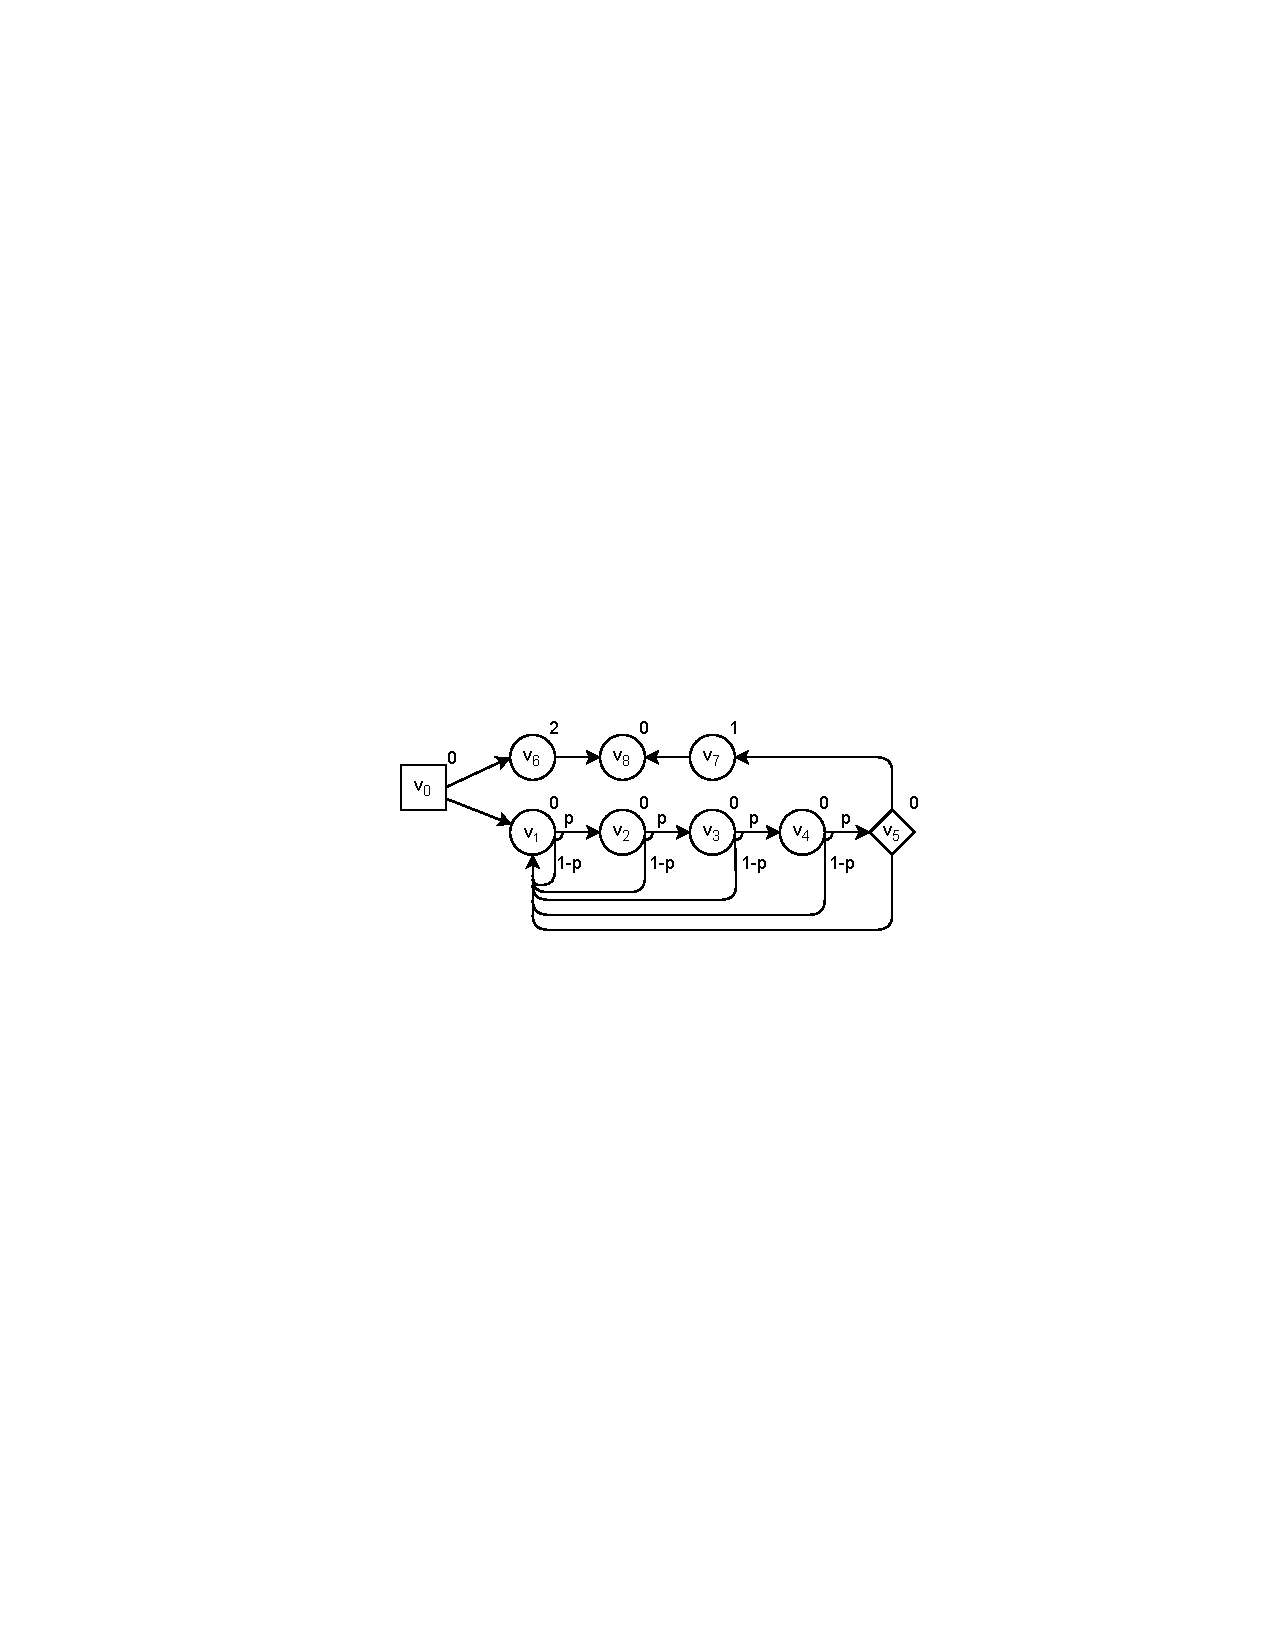
\includegraphics[scale=0.80]{Figs/prism-cex-1-horiz.pdf}%\hspace{1.5em}\mbox{}
\caption{Un simple juego de 2 jugadores: solo se muestran las probabilidades menores a 1.} \label{fig:prism-cex-1}
\end{figure}
Esta heurística podría devolver aproximaciones erróneas del mayor punto fijo. Ilustramos esto con un ejemplo sencillo. Considere el juego representado en la Figura~\ref{fig:prism-cex-1}. Para cualquier $\textsf{p}$, el valor del punto fijo más grande en el vértice $v_0$ es $2$. Sin embargo, al tomar $\textsf{p}=0.99$ y la tolerancia $\epsilon=10^{-6}$, {\Prism} devuelve un valor cercano a $39608$. %el valor $39607.955145476146$.
Esto ocurre porque {\Prism} cambia $0$ al valor $0.02$, lo que da como resultado un límite superior extremadamente grande.
%% Además, cada iteración solo produce una pequeña modificación en los valores %lo que arroja un valor final erróneo
%% lo que conduce a una convergencia incorrecta.
Obviamente, también devuelve una estrategia incorrecta para el vértice $v_0$. Hemos comprobado este ejemplo con nuestra herramienta y devolvió el valor correcto para el vértice $v_0$ en $2$ iteraciones, independientemente del valor de $\textsf{p}$.
%
Hemos elegido un valor grande para $\textsf{p}$ para que la diferencia sea notable. Los valores pequeños también pueden producir valores diferentes en, por ejemplo, $\textsf{v}_1$ solo que podría atribuirse a errores de aproximación.
%
%% Varying the relative error does not yield a better solution. In fact, taking $\epsilon = 10^{-8}$ {\Prism} returns a value closer to $2010051$.
%% \remarkPRD{Saque lo de las iteraciones porque no creo que agregue nada}
%% %a value of $2010050.7754585734$,  and also the number of iterations needed to compute such a value is increased: {\Prism} took $69508550$ iterations and $~30$ seconds with $\epsilon=10^{-8}$.}
%% Similar examples can be built to show that the upper bound estimated by {\Prism} could return a value smaller than the greatest fixpoint, yielding an incorrect final value.
%
También ejecutamos este operador en nuestros casos de estudio y observamos pequeñas diferencias en muchos de ellos (particularmente en Roborta) que aumentan cuando las probabilidades de falla también aumentan.




%% \subsection{{\Prism} Operators.} {\Prism} supports 2-player stochastic games,  therein properties are specified via the logic $\text{rPATL}$.This logic provides operators for expected rewards. Most of these operators are computed via a least fixpoint; thus, they are not comparable with our approach (they return $0$ in the case of a $0$-valued cycles).
%% Interestingly,  the operator  $\langle \langle p_1 \rangle \rangle \ \textsf{R}_{\text{max}{=}?}[\textsf{F}v]$ \remarkPRD{cambi\'e esto. Antes dec\'ia $\langle \langle p_1 \rangle \rangle \text{min}{=}?\textsf{R}[\textsf{F}v]$. Fijense que cambi\'e ``min'' por ``max''} returns the expected accumulated reward in which infinite plays receive an infinite value~\cite{DBLP:journals/fmsd/ChenFKPS13,DBLP:conf/cav/KwiatkowskaN0S20}.  {\Prism} approximates this value by computing a greatest fixpoint.  It uses a two-phase algorithm to do so:
%% \begin{enumerate}[(i)]
%% \item%
%%   it first replaces $0$-rewards by a small positive value and applies value iteration on this modification to get an estimated upper bound, and
%% \item%
%%   this upper bound is used to start another value iteration process aimed to compute the greatest fixpoint.
%% \end{enumerate}
%% %
%% \begin{wrapfigure}[10]{r}{55mm}
%% \vspace{-4ex}
%% %\fontsize{6.6}{6.6}\selectfont\ttfamily
%% \centering
%% 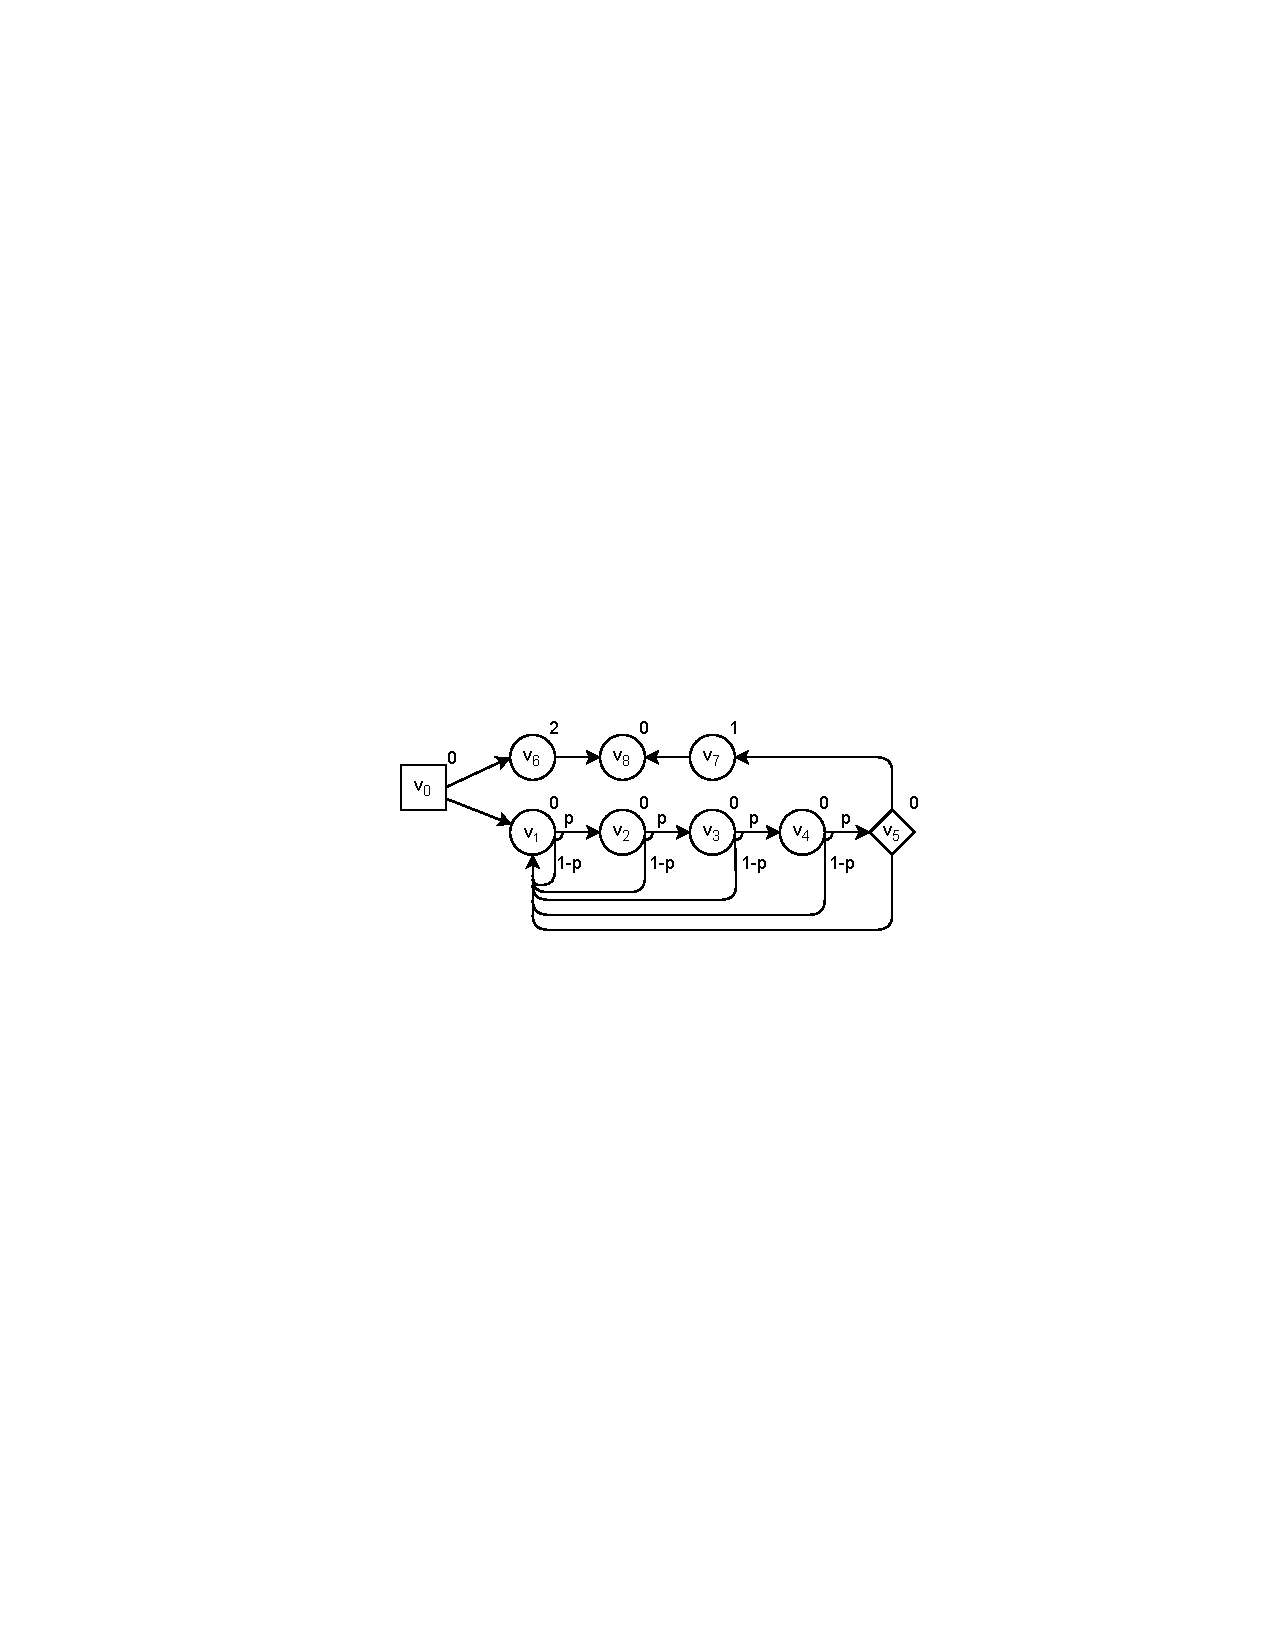
\includegraphics[scale=0.60]{Figs/prism-cex-1-horiz.pdf}%\hspace{1.5em}\mbox{}
%% \caption{A simple 2-player game: only probability less than 1 are shown.} \label{fig:prism-cex-1}
%% \end{wrapfigure}
%% This heuristic could return erroneous approximations of the greatest fixpoint.  We illustrate this with a simple example. Consider  the game depicted in Fig.~\ref{fig:prism-cex-1}, For any $T$, the value of the greatest fixpoint in vertex $v_0$ is $2$. However, by taking $T=0.99$ and tolerance $\epsilon=10^{-6}$, {\Prism} returns a value close to $39608$. %the value $39607.955145476146$.
%% This occurs because  {\Prism} changes $0$ by the value $0.02$, which results in an extremely large upper bound.  Furthermore, every iteration only produces a small modification in this value which yields an erroneous final value which leads to an incorrect convergence.   Obviously, it also returns an incorrect strategy for vertex $v_0$.  We have checked this example with our tool, and it returned the correct value for  vertex $v_0$ in $2$ iterations.
%% %
%% Varying the relative error does not yield a better solution. In fact, taking $\epsilon = 10^{-8}$ {\Prism} returns a value closer to $2010051$.
%% \remarkPRD{Saque lo de las iteraciones porque no creo que agregue nada}
%% %a value of $2010050.7754585734$,  and also the number of iterations needed to compute such a value is increased: {\Prism} took $69508550$ iterations and $~30$ seconds with $\epsilon=10^{-8}$.}
%% Similar examples can be built to show that the upper bound estimated by {\Prism} could return a value smaller than the greatest fixpoint, yielding an incorrect final value.


















Los \emph{Juegos estocásticos de camino mas corto} \cite{PatekBertsekas99} son juegos estocásticos de dos jugadores con recompensas (negativas o positivas) en los que las estrategias del minimizador se clasifican en \emph{adecuadas} e \emph{inadecuadas},
las estrategias adecuadas son las que aseguran la terminación. Como se demuestra en \cite{PatekBertsekas99}, estos juegos están determinados y ambos jugadores poseen estrategias óptimas sin memoria. Para probar estos resultados, los autores asumen que el valor esperado del juego para estrategias inadecuadas es $\infty$, esto asegura que el funcional correspondiente es una contracción y por lo tanto tiene un punto fijo único. Por el contrario, nos restringimos a recompensas no negativas pero no hacemos suposiciones sobre estrategias \textit{unfair}, como se mencionó anteriormente, la función correspondiente para nuestros juegos puede tener varios puntos fijos. Además, probamos que el valor del juego viene dado por el mayor punto fijo de $\Gamma$. En los últimos años, varios autores han investigado problemas estocásticos de camino más corto para MDPs (es decir, juegos de un solo jugador), donde se relaja la suposición sobre estrategias inadecuadas (por ejemplo, \cite{DBLP:conf/lics/Baier0DGS18}); hasta donde sabemos, estos resultados no se han extendido a los juegos de dos jugadores.

%% In \cite{SvorenovaKwiatkowska16}, a logical framework is presented for the verification and synthesis of systems. This framework combines probabilistic linear temporal logic with expected total, discounted, and average reward objective functions. 	The framework is implemented in the tool \Prism~\cite{DBLP:conf/cav/KwiatkowskaNP11}. Although a vast class of properties can be expressed in this framework, fairness assumptions over the environment are not dealt with in this line of research.
	
En \cite{DBLP:conf/ifipTCS/BolligC04} los autores abordan el problema de sintetizar un controlador que maximiza la probabilidad de satisfacer una propiedad {\LTL}. Las estrategias de \textit{fairness} se utilizan para reducir este problema a la síntesis de un controlador que maximiza una propiedad {\PCTL} sobre un juego producto. Sin embargo, este artículo no aborda las recompensas esperadas y la determinación del juego bajo supuestos de \textit{fairness}.

Curiosamente, en \cite{DBLP:conf/fossacs/AsarinCV10} los autores consideran el problema de ganar un juego de dos jugadores (no estocástico) con suposiciones de \textit{fairness} sobre el entorno. El objetivo del sistema es garantizar una propiedad $\omega$-regular. Los autores muestran que ganar en estos juegos es equivalente a ganar casi-seguramente en un proceso de decisión de Markov. Cabe señalar que este trabajo solo considera juegos no estocásticos. Además, las funciones de \textit{payoff} no se consideran allí.
%% Interestingly, in \cite{DBLP:conf/fossacs/AsarinCV10} the authors consider the problem of winning a (non-stochastic) two-player games with fairness assumptions over the environment. The objective of the system is to guarantee an $\omega$-regular property. The authors show that winning in these games is equivalent to almost-sure winning in a Markov decision process. It must be noted the aforementioned work only considers non-stochastic two-player games.  Furthermore, payoff functions are not considered therein.


        
%	The games introduced in \cite{Bacci0LM17,BacciBLMTB19,DesharnaisGJP04,DesharnaisLT11}  are based on probabilistic bisimulation, so they are symmetric. Furthermore, in \cite{DesharnaisGJP04,DesharnaisLT11} the nodes of the game graph are modeled using subsets of states of the PTSs, in our formulation
%we do not use subsets of states. The games defined in \cite{Bacci0LM17,BacciBLMTB19} use Kanterovich's and Hausdorff's liftings to deal with probabilistic distributions and non-determinism, respectively. In addition, the authors use the vertices of the transportation polytopes to model the probabilistic vertices. In contrast, we introduced a symbolic representation of games to avoid the state explosion caused by the vertices of the polytopes. Also note that the metrics introduced in \cite{Bacci0LM17,BacciBLMTB19} measure the (probabilistic) bisimulation distance between two PTSs, which for almost-sure failing systems is always $1$.
%		
%Another related framework is  defined in \cite{LanotteMT17}. Therein, the authors introduce a notion of weak simulation quasimetric tailored for reasoning about the evolution of \emph{gossip protocols}. This makes possible to compare network protocols that have similar behaviour up to a certain tolerance; being $0$ and $1$ the minimum and maximum distance, respectively.  Note that using this quasimetric to compare a network protocol with an almost-sure failing implementation will always return $1$, thus that approach cannot be used to quantify the masking fault-tolerance of almost-sure failing systems.
% 
% Finally, let us compare our approach with some metrics usual in fault-tolerance. \emph{Mean-Time To Failure} (MTTF) and \emph{Mean-Time Between Failures} (MTBF) \cite{ReliabilityBook}  capture the amount of time that a system is expected to be operative until it fails, and the expected elapsed time between failures, respectively.  These metrics are designed for hardware or electronic systems, where we have at hand estimations about the failure rate of the physical components. Our framework is designed to be used at a higher level of abstraction, where we have a model of the system to be implemented acting as a specification, and several possible implementations of it, described as probabilistic automata. This level of abstraction makes it possible to use this framework to analyze software fault-tolerance. Furthermore, note that our framework is particularly tailored to deal with masking fault-tolerance, a particular kind of fault-tolerance; in addition, our game formulation allows us to analyse systems on worst-case scenarios.

%\spnewtheorem*{proofofclaim}{Proof of claim}{\itshape}{\rmfamily}








%% \begin{proof}[of Theorem~\ref{thm:stopping-algorithm}]
%%   Recall the definitions of operators $\Apre$ and $\Epre$ for a given MDP $\MDP{H} = (V' , (V'_1,\emptyset, V'_\Probabilistic), \delta') $.
%% \begin{align*}
%% 	\Epre(C) \ = \ {}& \{ v \in V' \mid \delta'(v,C) > 0\} \\
%% 		      % & \cup \{ v \in  V'_1   \mid \exists v' \in V' : \delta'(v,v') * \delta(v', C) >0 \}\\
%% 	\Apre(C) \ = \ {} &\{ v \in V'_\Probabilistic  \mid \delta'(v,C) > 0\}
%% 		       \ \cup \ \{ v \in  V'_1   \mid \forall v' \in V' : \delta'(v,v') > 0 \Rightarrow v' \in C \}
%% \end{align*}
%% %
%% Furthermore, by considering that terminal vertices are absorbing, and let $T'$ be the terminal vertices of $\MDP{H}$, by Lemma 10.111 in~\cite{BaierK08}, we have that:
%% $\forall \strat{1} \in \Strategies{1}: \MDPProb{\strat{1}}_{\MDP{H},v}(\Diamond T') = 1$ iff $\inf_{\strat{1} \in \Strategies{1}} \MDPProb{\strat{1}}_{\MDP{H},v}(\Diamond T') = 1$ iff $v \in V' \setminus \Epre^*(V' \setminus \Apre^*(T'))$. 

%% %\remarkPC{add cite to Pedro's slides}\remarkPRD{Ah\'i puse la referencia apropiada}

%% Now, consider the MDP $\StochG^{\uniformstrat{2}}$, where $\uniformstrat{2}$ is the strategy defined in Theorem \ref{thm:uniform-prob}. Since $\uniformstrat{2}$ is memoryless, $\StochG^{\uniformstrat{2}}$ has the same vertices as $\StochG$ (the vertices in $V_2$ are considered as probabilistic vertices). Furthermore, note that $v \in  \AFairpre^*(C)$ (in game $\StochG$) iff
%% $v \in  \Apre^*(C)$ (in MDP $\StochG^{\uniformstrat{2}}$).
%% Then, $ v \in V\setminus \AFairpre^*(C)$ (in game $\StochG$) iff $v \in V \setminus \Apre^*(C)$ (in MDP $\StochG^{\uniformstrat{2}}$). 
%% That is, $ v \in \EFairpre^*(V \setminus \AFairpre^*(C))$ (in game $\StochG$)
%% iff $ v \in \Epre^*(V \setminus \Apre^*(C))$ (in MDP $\StochG^{\uniformstrat{2}}$), since $\Epre^*(S)$ and $\EFairpre^*(S)$ also coincide over 
%% any set of vertices. By the aforementioned property of MDPs, we have: 
%%  $\Prob{\strat{1}}{\uniformstrat{2}}_{\StochG,v}(\Diamond T) = 1$ for every $\strat{1} \in \Strategies{1}$  iff
%% $v \in \EFairpre^*(V \setminus \AFairpre^*(T))$. The  result follows by Theorem \ref{sec:fair-strats}.
%% \end{proof}
